\documentclass[10pt]{article}
\usepackage{graphicx} % Required for inserting images
\usepackage[a4paper,margin=2.2cm]{geometry}
\usepackage[ruled,vlined,linesnumbered]{algorithm2e}
\usepackage[T1]{fontenc}
\usepackage[utf8]{inputenc}
\usepackage{lmodern}
\usepackage{longtable}
\usepackage{microtype}
\usepackage{amsmath,amssymb,mathtools}
\usepackage{booktabs,tabularx,array,multirow}
\usepackage{enumitem}
\usepackage{appendix}
\usepackage{booktabs}
\usepackage{array}
\usepackage{xcolor}
\usepackage{tikz}
\usepackage{enumitem}
\usepackage{amsthm}
\usetikzlibrary{arrows.meta,
positioning,
fit,
shapes.geometric, 
backgrounds, 
calc}
\usepackage{listings}
\usepackage{hyperref}
\usepackage[nameinlink,noabbrev]{cleveref}
\usepackage{caption}
\usepackage{subcaption}
\usepackage{url}
\usepackage{balance}
\usepackage{tabularx}
\usepackage{booktabs}
\usepackage{array}
\usepackage{makecell}
\usepackage{ragged2e}

\newcolumntype{C}[1]{>{\Centering\arraybackslash}p{#1}}
\newcolumntype{Y}{>{\RaggedRight\arraybackslash}X}

\definecolor{acmblue}{RGB}{37,80,130}
\definecolor{acmgray}{RGB}{245,247,249}
\definecolor{passgreen}{RGB}{34,139,34}
\definecolor{deviationorange}{RGB}{210,105,30}
\definecolor{skipgray}{RGB}{105,105,105}
\definecolor{failred}{RGB}{178,34,34}
\definecolor{alertred}{RGB}{178,34,34}
\definecolor{preservedgreen}{RGB}{34,139,34}
\definecolor{approximatedorange}{RGB}{210,105,30}
\definecolor{unsupportedgray}{RGB}{105,105,105}
\hypersetup{
  colorlinks=true,
  linkcolor=acmblue,
  citecolor=acmblue,
  urlcolor=acmblue,
  pdftitle={Agentic Configuration Management},
  pdfauthor={AUTHOR NAME}
}

\lstdefinestyle{acmcode}{
  basicstyle=\ttfamily\small,
  backgroundcolor=\color{acmgray},
  frame=single,
  rulecolor=\color{black!15},
  breaklines=true,
  columns=fullflexible,
  showstringspaces=false
}

\newcommand{\acmcore}{\textsc{ACM Core}}
\newcommand{\framework}{framework-independent}
\newcommand{\todo}[1]{\textcolor{red}{[TODO: #1]}}
\newcommand{\system}{\mathcal{S}}
\newcommand{\configgraph}{G_C}
\newcommand{\runtimegraph}{G_R}
\newcommand{\assurancegraph}{G_A}
\newcommand{\evolutiongraph}{G_E}
\newcommand{\statuspass}{\textcolor{passgreen}{\texttt{pass}}}
\newcommand{\statusdeviation}{\textcolor{deviationorange}{\texttt{pass\_with\_deviation}}}
\newcommand{\statusskip}{\textcolor{skipgray}{\texttt{skipped}}}
\newcommand{\statusfail}{\textcolor{failred}{\texttt{fail}}}
\newcommand{\statusnotexec}{\texttt{not\_executed}}
\newcommand{\statuspreserved}{\textcolor{preservedgreen}{\texttt{preserved}}}
\newcommand{\statusapproximated}{\textcolor{approximatedorange}{\texttt{approximated}}}
\newcommand{\statusunsupported}{\textcolor{unsupportedgray}{\texttt{unsupported}}}

\newtheorem{theorem}{Theorem}
\newtheorem{lemma}{Lemma}
\newtheorem{proposition}{Proposition}

\title{\textbf{Agentic Configuration Management (ACM):\\A Reference Configuration Model for Governed Agentic Systems}}

\author{
  Audrey Quessadda-Vial\\
  PwC\\
  \texttt{audrey.quessada-vial@pwc.com}
}

\date{Draft --- August 2026}

\begin{document}

\maketitle

\begin{abstract}

Agentic systems are rapidly evolving from isolated LLM applications to complex software composed of interacting agents, tools, prompts, skills, composite subsystems, models, and execution workflows. While existing LLMOps and AgentOps platforms provide valuable support for orchestration and observability, they do not offer a framework-independent configuration model capable of describing, validating, and governing the system as a coherent whole. As a result, configuration management remains fragmented across frameworks, making reproducibility, impact analysis, and long-term maintenance increasingly difficult.

This paper introduces \textbf{Agentic Configuration Management (ACM)}, a framework-independent, revision-aware reference configuration model capable of representing heterogeneous agentic systems and relating governed configurations to runtime observations through explicit governance semantics. ACM extends established Software Configuration Management principles to the agentic domain through immutable configuration items, explicit baselines, lifecycle management, dependency-aware state propagation, and runtime provenance. Rather than replacing existing orchestration frameworks, ACM provides a common representation that enables their configurations to be normalized and managed consistently.

We describe a complete reference implementation in Python together with adapters for LangGraph, CrewAI and OpenAI Agents SDK. The implementation includes a deterministic validation engine, a replayable event model, and a preservation-based extraction process that reconstructs native workflows into the ACM representation. The evaluation combines normative scenarios with automated tests to assess both the consistency of the model and the fidelity of the extraction process across frameworks.

We also developed a proof of termination—including the uniqueness of the fixed point—for the propagation of modification impacts, as well as a quantitative analysis of these impacts. 

The results show that ACM can preserve the structural information required for configuration governance while making explicit the information that is approximated or unavailable in the underlying framework. These results provide initial evidence that a unified configuration model can support reproducibility, auditability, and governance across heterogeneous agentic ecosystems without being tied to a specific orchestration framework.

\end{abstract}

\section{Introduction}

Agentic AI systems are rapidly evolving from isolated large language model (LLM) applications into complex software systems composed of interacting autonomous components. Their behaviour increasingly depends on configurable artifacts that evolve throughout both development and execution, making configuration governance substantially more challenging than in traditional software systems \cite{bersoff1978software, bersoff1984elements, whitgift1991methods}. As these systems become larger, more dynamic, and more heterogeneous, ensuring their reproducibility, auditability, and controlled evolution has emerged as a fundamental engineering challenge \cite{Hughes03072025, pandey2025agentic}.

Although current agentic ecosystems provide powerful execution capabilities, the representation of system configurations remains largely framework-specific \cite{bandi2025rise}. Configuration information is distributed across heterogeneous abstractions, lifecycle conventions, and runtime representations that differ from one framework to another \cite{acharya2025agentic, Inioluwa2020}. As a consequence, comparing, auditing, evolving, or reproducing agentic systems independently of their execution environment remains difficult.

This situation exposes a gap between the maturity of Software Configuration Management (SCM) principles and their application to modern agentic systems. Established SCM concepts such as immutable revisions, controlled baselines, change management, provenance, and configuration auditing have proven their effectiveness for conventional software engineering \cite{ieee2012ieee, leon2015software, amershi2019}, yet they have not been systematically adapted to the governance of agentic configurations.

This paper introduces \textbf{Agentic Configuration Management (ACM)}, a framework-independent governance representation for governing the configuration of agentic systems. ACM provides a common configuration representation that complements existing execution frameworks by supporting configuration governance, traceability, reproducibility, and controlled evolution across heterogeneous implementations.

A central design principle of ACM is the explicit separation between governed configurations and their operational realization. Configuration describes the intended, versioned, and governed structure of an agentic system independently of any execution framework, whereas runtime represents one particular execution of that configuration under specific operational conditions. ACM governs the former and provides semantic mechanisms for relating it to the latter without conflating the two. This distinction constitutes the conceptual foundation of ACM and motivates the separation between configuration governance and execution semantics developed throughout the remainder of the paper.

\begin{figure*}[t]
	\centering
	
\includegraphics[width=0.7\textwidth]{figures/ACM_architecture_principles.png}
	\caption{Positioning of ACM. ACM acts as a framework-independent configuration layer that connects agent frameworks (orchestration), LLMOps platforms (observability and evaluation) and deployment environments (execution).}
	\label{fig:ACM_positioning}
\end{figure*}

ACM focuses on governing the former while providing formal semantics to interpret the latter relative to the governed configuration. The contributions of this paper are fourfold:

\begin{itemize}
    \item We propose a \textbf{framework-independent governance representation} that defines the core concepts, relationships, and abstractions required to represent governed heterogeneous agentic configurations.
    
    \item We formalize the \textbf{governance semantics} of agentic configurations through lifecycle models, state propagation, assurance semantics, and runtime governance mechanisms.
    
    \item We present a \textbf{reference operationalization} of the model, including a Python reference implementation together with projection mechanisms for heterogeneous agentic frameworks.
    
    \item We evaluate the \textbf{expressiveness and operational feasibility} of the proposed model through normative scenarios, automated validation, quantitative impact analysis and cross-framework projection experiments.
\end{itemize}

The remainder of this paper is organized as follows. Section~\ref{sec:related_work} reviews the foundations of Software Configuration Management, AI governance, LLMOps, AgentOps, and agentic frameworks, and identifies the gap addressed by the Agentic Configuration Model (ACM). Section~\ref{sec:design_principles} derives the design principles of the proposed reference model. Section~\ref{sec:reference_model} introduces the ACM reference model, while Section~\ref{sec:governance_semantics} formalizes its governance semantics. Section~\ref{sec:operationalization} describes its operationalization through a reference architecture, framework adapters, governance algorithms, and a reference implementation. Section~\ref{sec:evaluation} evaluates the proposed model. Finally, Sections~\ref{sec:discussion}, \ref{sec:threats_validity}, \ref{sec:future_work}, and \ref{sec:conclusion} discuss the implications, limitations, future research directions, and conclusions of this work.

\section{Related Work}
\label{sec:related_work}

\subsection{Software Configuration Management}
\label{sec:scm}

Software Configuration Management (SCM) provides the engineering foundations for identifying, controlling, and auditing the evolution of software systems. Rather than focusing solely on version control, SCM defines a disciplined process for establishing configuration baselines, managing change, maintaining traceability, and ensuring that released systems remain reproducible and auditable throughout their lifecycle \cite{whitgift1991methods, conradi1998version, leon2015software, bersoff1984elements, bersoff1978software}.

These principles have been formalized by long-established standards and bodies of knowledge, including IEEE~828, ISO/IEC/IEEE~12207, and the \emph{Software Engineering Body of Knowledge} (SWEBOK) \cite{swebok40, ieee2012ieee, wohlinsnowballing}. Although these references differ in scope, they consistently describe configuration management as a combination of configuration identification, change control, configuration status accounting, and configuration verification and audit.

Classical SCM has proved effective for conventional software systems composed of relatively stable software artifacts such as source code, libraries, documentation, build configurations, and release packages \cite{chacon2014pro}. Its central concepts---configuration items, immutable baselines, controlled revisions, dependency management, and change auditing---provide the foundations required to ensure consistency and reproducibility across software releases.

\begin{figure*}[t]
	\centering
	
\includegraphics[width=0.7\textwidth]{figures/SCM_configuration_management_liefcycle_baseline.png}
	\caption{Fundamental Software Configuration Management (SCM) process. Configuration identification, change control, configuration status accounting, and configuration verification and audit constitute the four core SCM activities defined by established software engineering standards. Together, they provide the conceptual foundations for immutable revisions, controlled baselines, traceability, and governance that are extended by ACM to heterogeneous agentic systems \cite{bersoff1984elements}.}
	\label{fig:SCM_framework}
\end{figure*}

However, applying these principles directly to agentic systems is not straightforward. In addition to executable software components, agentic systems rely on heterogeneous configurable artifacts, dynamic execution structures, and runtime-generated elements that are not explicitly addressed by traditional SCM models. Consequently, while SCM provides the conceptual foundations for configuration governance, additional abstractions are required to represent and govern the configuration of modern agentic systems.

\subsection{AI Governance}
\label{sec:ai_governance}

The rapid adoption of AI systems has expanded governance concerns beyond traditional software engineering. Recent standards, regulatory frameworks, and technical initiatives emphasize accountability, transparency, risk management, and auditability throughout the AI lifecycle \cite{pandey2025agentic, Engin_Hand_2026, Gangavarapu2025, shavit2023practices, IMDA2026AgenticMGF}. Although these initiatives differ in scope, they share the objective of ensuring that AI systems remain trustworthy, traceable, and subject to appropriate organizational oversight.

From the perspective of agentic systems, three complementary areas are particularly relevant: governance frameworks defining organizational requirements, provenance mechanisms ensuring artifact traceability, and emerging approaches dedicated to the governance of autonomous agents. Together, these perspectives establish important governance objectives but do not define a common configuration representation for heterogeneous agentic systems.

\subsubsection{Governance Frameworks}
\label{sec:governance_frameworks}

Several governance frameworks have established principles for the responsible development and operation of AI systems. Examples include the NIST AI Risk Management Framework (AI RMF), ISO/IEC~42001, ISO/IEC~23894, the OECD AI Principles, and the European AI Act \cite{ai2023artificial, benraouane2024ai, simonetta2024iso, yeung2020recommendation, edwards2021eu}. While their objectives and intended audiences differ, they consistently emphasize governance practices such as accountability, documentation, risk management, human oversight, traceability, and auditability.

These frameworks define organizational objectives and governance processes rather than implementation models. They describe \emph{what} should be governed and documented but intentionally remain independent of the internal representation adopted by AI platforms or execution frameworks. Consequently, they do not provide a framework-independent configuration model capable of representing the complete structure and evolution of an agentic system.

\subsubsection{Provenance and Software Supply Chain}
\label{sec:provenance_supply_chain}

Provenance has become a fundamental requirement for software and AI governance. Existing standards and specifications, including W3C PROV, Software Bills of Materials (SBOMs), SPDX, and the Supply-chain Levels for Software Artifacts (SLSA) \cite{missier2013w3c, SBOM10336262, stewart2010software, okafor2022sok, cobbe2023understanding}, improve traceability by documenting artifact origins, dependencies, integrity, and production processes. These mechanisms strengthen reproducibility, software supply-chain security, and compliance by making software artifacts and their relationships explicitly traceable.

Although highly valuable, these approaches primarily describe software packages, build processes, datasets, or deployment artifacts. They do not represent the semantic configuration of agentic systems, whose behavior depends on heterogeneous configuration artifacts such as agents, prompts, models, skills, composite subsystems, tools, policies, and dynamically evolving execution structures. Consequently, provenance alone is insufficient to govern the configuration of an entire agentic system.

\subsubsection{Governance of Agentic Systems}
\label{sec:agentic_governance}

The emergence of agentic AI has stimulated research on governance mechanisms specifically targeting autonomous and multi-agent systems. Existing approaches typically address runtime supervision, policy enforcement, authorization, monitoring, safety constraints, or operational accountability. Likewise, current AgentOps and orchestration platforms increasingly provide tracing, evaluation, and operational monitoring capabilities for agent execution but are framework-dependent (see Section ~\ref{sec:llmops_agentops}).

This observation complements the limitations identified in classical Software Configuration Management and motivates the need for a unified configuration reference model that separates configuration governance from execution concerns. This gap forms the foundation of the Agentic Configuration Management (ACM) reference model introduced in the following sections.

\subsection{LLMOps and AgentOps}
\label{sec:llmops_agentops}

The emergence of large language models has also given rise to a new generation of operational platforms dedicated to managing AI applications throughout their lifecycle. Inspired by established MLOps practices, LLMOps extends operational support to applications built around foundation models by providing capabilities for prompt management, experimentation, evaluation, deployment, monitoring, and observability. As agentic systems have become increasingly dynamic and autonomous, these practices have naturally evolved toward AgentOps, which addresses the operational management of multi-agent applications and long-running agentic workflows \cite{cesarano2026grand, shavit2023practices, pandey2025agentic, dumas2026}.

Unlike traditional software configuration management, LLMOps and AgentOps focus primarily on the operational lifecycle of AI applications rather than on the governance of their underlying configurations \cite{pahune2025transitioning, amershi2019, dong2024agentops}. Their objective is to facilitate development, deployment, monitoring, experimentation, and continuous improvement while maintaining visibility over system behavior during execution.

Although terminology varies across platforms, most LLMOps and AgentOps solutions converge toward a common set of operational capabilities, including prompt management, execution tracing, evaluation workflows, observability, deployment management, and experiment tracking. These capabilities provide the operational evidence required to understand how an AI application behaves in production and to support iterative improvements of prompts and workflows.

From the perspective of configuration governance, several concepts introduced by these platforms are particularly relevant. 

\begin{itemize}
	\item Configuration management concerns the explicit representation of configurable artifacts and their versions \cite{liu2025towards, Hughes03072025, langfusedocs, heliconedocs}. 
	\item Provenance records the origin and derivation history of these artifacts.
	\item Lineage captures the dependency relationships connecting successive versions, execution traces, and derived artifacts \cite{cesarano2026grand, rajath2025review}. 
	\item Tracing records the sequence of execution events occurring during system operation.
	\item Observability \cite{langsmithdocs} aggregates telemetry that enables operators to inspect the internal behavior of deployed applications \cite{opentelemetry}. 
	\item Deployment state characterizes the operational status of a configuration once deployed within a target environment \cite{braintrustdocs}.
\end{itemize}	

These concepts constitute essential building blocks for governing modern AI applications. However, they generally remain attached to operational artifacts such as prompts, traces, evaluations, or deployments, rather than providing a unified representation of the complete configuration of an agentic system. Relationships among agents, prompts, models, tools, skills, composite subsystems, policies, workflows, and runtime-generated components are typically represented through platform-specific abstractions, preventing the establishment of a framework-independent configuration model.

Representative platforms illustrate this evolution. Prompt management solutions increasingly support prompt versioning, labels, rollback, experimentation, and deployment workflows. Observability platforms provide execution traces, telemetry, evaluation pipelines, and runtime analytics. More recent AgentOps environments extend these capabilities to multi-agent executions through richer runtime monitoring, workflow inspection, and execution replay \cite{sahir2026agentops}. 

As an example of open-source observability platform, we can cite LangFuse~\cite{langfusedocs} providing prompt management, execution tracing, evaluation, experimentation, and prompt versioning. It enables developers to associate prompt revisions with runtime traces, datasets, and evaluation results, thereby improving reproducibility and experimentation across LLM-based applications. 
Another observability platform is Helicone ~\cite{heliconedocs}. It supports request tracing, prompt versioning, experimentation, evaluation, and deployment management. Its primary focus is operational monitoring and prompt-centric development workflows, providing valuable runtime telemetry and performance insights. 

Together, these platforms substantially improve the operational governance of AI applications but remain centered on execution management rather than on the governance of configuration itself, nevertheless they do no aim at representing the complete configuration of heterogeneous agnetic system (see Table ~\ref{tab:llmops_comparison} for a governance capability comparison between the current LLMOPs and AgentOps platforms).

\begin{table*}[t]
\centering
\caption{Representative capabilities of current LLMOps and AgentOps platforms. The comparison highlights their primary focus on operational lifecycle management rather than framework-independent configuration governance.}
\label{tab:llmops_comparison}

\renewcommand{\arraystretch}{1.15}
\begin{tabular}{p{4.2cm}ccccc}
\toprule
\textbf{Capability} &
\textbf{LangSmith} &
\textbf{LangFuse} &
\textbf{Helicone} &
\textbf{Braintrust} &
\textbf{PromptLayer} \\
\midrule

Prompt versioning                & \checkmark & \checkmark & \checkmark & \checkmark & \checkmark \\

Prompt deployment / labels       & $\sim$ & \checkmark & \checkmark & $\sim$ &  \checkmark \\

Execution tracing                & \checkmark & \checkmark & \checkmark & \checkmark & \checkmark \\

Observability / telemetry        & \checkmark & \checkmark & \checkmark & \checkmark & $\sim$ \\

Evaluation workflows             & \checkmark & \checkmark & \checkmark & \checkmark & $\sim$ \\

Experiment tracking              & \checkmark & \checkmark & \checkmark & \checkmark & $\sim$ \\

Prompt provenance                & $\sim$ & \checkmark & \checkmark & $\sim$ & \checkmark \\

Execution lineage                & \checkmark & \checkmark & \checkmark & \checkmark & $\sim$ \\

Deployment state                 & $\sim$ & \checkmark & \checkmark & $\sim$ & \checkmark \\

Runtime replay                   & \checkmark & $\sim$ & $\sim$ & $\sim$ & $\sim$ \\

Framework-specific integrations  & \checkmark & \checkmark & \checkmark & \checkmark & \checkmark \\

\midrule

Framework-independent configuration model
                                 & -- & -- & -- & -- & -- \\

Configuration graph              & -- & -- & -- & -- & -- \\

Immutable configuration baseline & -- & -- & -- & -- & -- \\

Configuration lifecycle          & -- & -- & -- & -- & -- \\

Configuration dependency model   & -- & -- & -- & -- & -- \\

Governed configuration revisions & -- & -- & -- & -- & -- \\

Configuration state propagation  & -- & -- & -- & -- & -- \\

Configuration governance semantics
                                 & -- & -- & -- & -- & -- \\

\bottomrule
\end{tabular}

\vspace{1mm}

\footnotesize
$\checkmark$ Supported \hspace{1em}
$\sim$ Partial support \hspace{1em}
-- Not provided as a first-class capability.

\end{table*}

\subsection{Agentic Frameworks}
\label{sec:agentic_frameworks}

The rapid adoption of agentic AI has led to the emergence of numerous frameworks dedicated to designing and executing autonomous or multi-agent applications. Although their architectures differ, these frameworks share a common objective: orchestrating the execution of agents, coordinating interactions among heterogeneous components, and integrating large language models with external tools, memory, and user-defined workflows (non exhaustive list of frameworks \cite{crewaidocs, langgraphdocs, googleadkdocs, microsoftadkdocs, openaiddocs, claudedocs, mistraldocs}).

Current frameworks cover a broad spectrum of orchestration paradigms. Some adopt explicit graph-based execution models, while others organize applications around agents, tasks, crews, or conversational interactions. Despite these architectural differences, they generally provide abstractions for defining execution flows, invoking tools, managing shared or local state, and coordinating agent interactions during runtime (see Table ~\ref{tab:framework_comparison} in Appendix ~\ref{appendix:related_work}).

Beyond execution, modern frameworks increasingly incorporate operational capabilities such as checkpointing, persistence, human-in-the-loop interactions, execution replay, and integration with observability platforms. These features considerably simplify the development and deployment of agentic applications and complement the operational services provided by LLMOps and AgentOps platforms.

However, the internal representations adopted by these frameworks remain closely coupled to their respective execution models. Configuration artifacts, dependency structures, lifecycle conventions, and runtime abstractions are expressed through framework-specific concepts that are not directly interoperable. Consequently, while these frameworks provide rich execution semantics, they do not define a common representation suitable for governing configurations independently of a particular execution environment.



\subsection{Gap Analysis}
\label{sec:gap_analysis}

The preceding sections have examined complementary perspectives on the governance of AI systems, including Software Configuration Management, AI governance frameworks, LLMOps and AgentOps platforms, and agentic execution frameworks. Although these approaches address different aspects of the AI lifecycle, they collectively contribute to the governance of modern AI applications. However, they cannot simply be combined to obtain a unified configuration-governance solution. Software Configuration Management governs software artifacts but has no framework-independent representation of agentic abstractions. AI governance frameworks define organizational objectives and compliance requirements without specifying a configuration model. LLMOps and AgentOps platforms provide observability, evaluation, and operational tooling, while execution frameworks define runtime semantics through framework-specific abstractions. 

Because each family addresses a different governance concern and relies on its own representation of the system, no common semantic model exists for representing, versioning, and governing heterogeneous agentic configurations independently of their execution environment.
This observation motivates the need for a framework-independent reference configuration model capable of integrating these complementary perspectives while preserving a stable governance representation across heterogeneous agentic ecosystems.

Table~\ref{tab:gap_analysis} synthesizes the coverage of representative governance capabilities across these complementary families of approaches. Rather than comparing the approaches themselves, the analysis evaluates the extent to which each family addresses the governance capabilities required throughout the lifecycle of agentic systems.

\begin{table*}[t]
\centering
\caption{Coverage of representative governance capabilities across complementary families of approaches. A detailed comparison is provided in Appendix Table ~\ref{tab:gap_analysis_detailed}.}
\label{tab:gap_analysis}

\renewcommand{\arraystretch}{1.15}

\begin{tabular}{p{5.2cm}ccccc}
\toprule
\textbf{Governance Capability}
&
\textbf{SCM}
&
\textbf{AI Gov.}
&
\textbf{LLMOps / AgentOps}
&
\textbf{Frameworks}
\\
\midrule

Configuration identification          & \checkmark & $\sim$ & $\sim$ & $\sim$ \\

Version management                    & \checkmark & -- & $\sim$ & $\sim$ \\

Configuration provenance              & $\sim$ & \checkmark & \checkmark & $\sim$ \\

Dependency traceability               & \checkmark & $\sim$ & \checkmark & $\sim$ \\

Execution observability               & -- & $\sim$ & \checkmark & \checkmark \\

Lifecycle governance                  & $\sim$ & \checkmark & $\sim$ & $\sim$ \\

Framework-independent representation  & -- & -- & -- & -- \\

Unified configuration model           & -- & -- & -- & -- \\

\bottomrule
\end{tabular}

\vspace{1mm}

\footnotesize
$\checkmark$ Fully addressed \hspace{1em}
$\sim$ Partially addressed \hspace{1em}
-- Not addressed as a primary capability.

\end{table*}

The limitation of combining these approaches is therefore not the absence of governance, observability, execution, or compliance mechanisms. Rather, these capabilities remain distributed across complementary technologies that operate on different abstractions and representations. As a result, governed configurations cannot be represented, versioned, compared, and evolved through a common semantic model independently of the underlying execution framework. Our reference model ACM addresses this missing abstraction layer by introducing a framework-independent reference configuration model that unifies configuration governance while remaining complementary to existing execution frameworks, LLMOps platforms, AgentOps solutions, and organizational AI governance frameworks. These observations provide the rationale for designing a unified reference model which is presented in the next section. It establishes the requirements for a unified reference model dedicated to configuration governance for agentic systems (see next Section ~\ref{sec:design_principles}).

\section{Design Principles}
\label{sec:design_principles}

Rather than extending an existing orchestration framework or operational platform, the objective of ACM is to establish a reference model that complements these ecosystems while remaining independent of their implementation technologies. ACM addresses therefore a complementary concern by representing governed configurations independently of execution platforms, enabling immutable baselines, dependency-aware configuration management, and explicit relationships between configuration revisions, runtime observations, and assurance evidence.

The design of such a reference model is guided by a set of requirements derived from the limitations identified in the preceding analysis. These principles define the properties that any framework-independent configuration governance model should satisfy. They intentionally describe design requirements rather than implementation choices; the conceptual realization of these principles is introduced in Section~\ref{sec:reference_model}.

Table~\ref{tab:design_principles} summarizes the seven principles that guide the design of ACM.
\begin{table*}[t]
\centering
\caption{Design principles guiding the ACM reference model.}
\label{tab:design_principles}

\renewcommand{\arraystretch}{1.15}

\begin{tabular}{p{1.0cm}p{4.0cm}p{9.2cm}}
\toprule
\textbf{ID} &
\textbf{Principle} &
\textbf{Objective}
\\
\midrule

P1 &
Framework Independence &
Remain independent of execution frameworks, orchestration engines, and AI providers.\\

P2 & Explicit Configuration Representation & Represent every configurable artifact explicitly under configuration governance.\\

P3 &  Immutable Versioning & Ensure deterministic evolution through immutable revisions and controlled baselines. \\

P4 & Configuration–Execution Separation & Clearly distinguish governed configurations from runtime execution.\\

P5 & Explicit Traceability & Preserve provenance and dependency relationships throughout the configuration lifecycle.\\

P6 & Governance by Design & Support lifecycle governance, policy enforcement, assurance, and auditability.\\

P7 & Extensibility & Allow the reference model to evolve without changing its governance foundations.
\\
\bottomrule
\end{tabular}

\end{table*}

\paragraph{P1 -- Framework Independence}

A configuration governance model shall remain independent of any specific orchestration framework, execution engine, or AI provider. Heterogeneous agentic systems should therefore be representable through a common abstraction that preserves governance semantics without exposing framework-specific implementation details. This independence enables interoperability across evolving ecosystems while avoiding dependence on a particular execution technology.

\paragraph{P2 -- Explicit Configuration Representation}

Every artifact whose definition influences the behaviour of an agentic system shall be represented explicitly as a governed configuration object. The model should support heterogeneous artifacts while remaining independent of their implementation and execution semantics.

\paragraph{P3 -- Immutable Versioning}

Configuration evolution shall rely on immutable revisions. Every modification shall produce a new governed revision while preserving previous versions to ensure reproducibility, auditability, and deterministic reconstruction of historical configurations.

\paragraph{P4 -- Configuration--Execution Separation}

Configuration governance shall remain conceptually independent from runtime execution. Runtime observations may enrich governance information but shall not directly modify governed configurations.

\paragraph{P5 -- Explicit Traceability}

The model shall preserve explicit traceability among governed artifacts throughout their lifecycle. Structural dependencies, provenance relationships, and configuration evolution should remain observable and auditable independently of any execution framework.

\paragraph{P6 -- Governance by Design}

Governance shall be an intrinsic property of the configuration model rather than an external operational concern. The model should support lifecycle control, policy evaluation, assurance, auditability, and deterministic governance decisions.

\paragraph{P7 -- Extensibility}

The reference model shall remain extensible to accommodate future categories of configuration artifacts, governance policies, and execution paradigms without modifying its fundamental governance principles.


The following section introduces the ACM reference model, which operationalizes these principles through a normalized representation of governed configuration artifacts and their relationships.

\section{ACM Reference Model}
\label{sec:reference_model}

The ACM is made to offer a common governance layer capable of representing heterogeneous configuration artifacts independently of their execution environment.

The model is designed around three complementary objectives. First, it provides a unified representation of configurable artifacts participating in an agentic system. Second, it explicitly captures the structural and governance relationships among these artifacts. Third, it establishes the conceptual foundations required to support lifecycle management, traceability, provenance, auditability, and configuration evolution.

Section~\ref{sec:conceptual_overview} introduces the conceptual organization of the model. Section~\ref{sec:aci_model} defines the abstract representation of Agentic Configuration Items (ACIs). The following subsections specify the relationships between ACIs, baseline composition, and the structural properties of the reference model.


\subsection{Conceptual Overview}
\label{sec:conceptual_overview}

An agentic system is composed of numerous configurable artifacts originating from heterogeneous technologies, including orchestration frameworks, language models, prompts, tools, skills, composite subsystems, policies, execution environments, and governance mechanisms. Although these artifacts collectively determine the behaviour of the system, they are generally represented through framework-specific abstractions and governed independently.

The ACM reference model introduces a unified conceptual representation in which every configurable artifact is treated as a governed configuration item, regardless of its implementation technology or execution framework. This abstraction enables heterogeneous artifacts to be managed according to a common governance model while preserving their individual semantics.

Rather than organizing configuration items according to implementation technologies, ACM structures them according to the governance role they fulfil within the system. Configuration items are therefore organized into three conceptually independent families:

\begin{itemize}

\item \textbf{Structural items}, which describe the static composition of the system and its configurable artifacts.

\item \textbf{Governance items}, which define policies, assurance evidence, compliance constraints, and lifecycle governance.

\item \textbf{Runtime items}, which represent execution-related information generated during system operation while remaining linked to the governed configuration.

\end{itemize}

Although these families are conceptually independent, they remain connected through explicit relationships that preserve traceability across the complete lifecycle of the system. This organization separates structural configuration, governance information, and runtime observations while allowing each perspective to evolve independently.

To represent these complementary perspectives, ACM organizes configuration information into four interconnected conceptual graphs, illustrated in Figure~\ref{fig:acm_reference_model}.

\begin{itemize}

\item The \textbf{Configuration Graph} represents the governed configuration of the agentic system and the structural relationships among configuration items.

\item The \textbf{Assurance Graph} captures governance policies, assurance evidence, compliance constraints, and policy enforcement.

\item The \textbf{Runtime Graph} represents execution observations generated during system operation while maintaining explicit links to governed configuration items.

\item The \textbf{Evolution Graph} provides an integrated view of configuration evolution and history from a baseline.

\end{itemize}

The decomposition into four complementary graphs is a deliberate design decision rather than a modeling convenience. Each graph addresses a distinct governance concern that follows its own semantics and lifecycle. Separating these orthogonal concerns preserves conceptual clarity, avoids mixing static and dynamic governance information, and enables each graph to evolve independently while remaining linked through explicit traceability relationships. 

\begin{figure*}[t]
	\centering
	
\includegraphics[width=0.6\textwidth]{figures/ACM_reference_model.png}
	\caption{Multi-graph organization of the ACM reference model. Configuration, evolution, runtime, and assurance are represented as four complementary governance views that share the same immutable configuration revisions. This separation allows each graph to evolve according to its own semantics while maintaining explicit consistency and traceability through a common revision space.}
	\label{fig:acm_reference_model}
\end{figure*}

\subsection{Agentic Configuration Item}
\label{sec:aci_model}

The Agentic Configuration Item (ACI) is the fundamental abstraction of the ACM reference model. An ACI represents any configurable artifact whose definition contributes to the specification, governance, or execution of an agentic system. By introducing a common abstraction independent of implementation technologies, ACM enables heterogeneous artifacts originating from different frameworks to be represented and governed uniformly.

Unlike traditional software configuration items, which primarily describe software artifacts, ACIs encompass the broader range of configurable elements required by modern agentic systems. Examples include agents, prompts, skills, composite subsystems, workflows, tools, language models, policies, assurance evidence, runtime observations, and other governance artifacts. Although these artifacts differ in purpose and lifecycle, they share a common representation within the ACM reference model (see Figure ~\ref{fig:aci_metamodel}).

Every ACI is represented as an immutable configuration revision. Once created, the content associated with a revision never changes; any modification results in the creation of a new revision while preserving previous versions for reproducibility, auditability, and deterministic reconstruction of historical configurations. Configuration evolution is therefore represented explicitly through successive governed revisions rather than mutable objects.

An ACI combines three complementary dimensions:

\begin{itemize}

\item an immutable configuration content describing the governed artifact;

\item an identity and revision model ensuring uniqueness, version management, and reproducibility;

\item governance metadata describing lifecycle information, provenance, integrity, and other management attributes required for configuration governance.

\end{itemize}

This representation intentionally separates the conceptual identity of a configuration item from the successive revisions describing its evolution. A configuration item therefore exists independently of any particular revision, while each revision represents a complete immutable state of that item at a specific point in its lifecycle.

To accommodate the diversity of configurable artifacts encountered in agentic systems, ACIs are organized into three conceptually independent families introduced in Section~\ref{sec:conceptual_overview}: Structural ACIs, Governance ACIs, and Runtime ACIs. These families share the same abstract representation while specializing the governed content according to the role performed by each artifact within the reference model. This specialization enables the model to remain extensible without introducing family-specific governance mechanisms.

Figure~\ref{fig:aci_metamodel} presents the abstract representation of an Agentic Configuration Item. The following subsections specify its attributes, relationships, and composition rules.

\begin{figure*}[t]
	\centering
	
\includegraphics[width=\textwidth]{figures/ACI_metamodel_old.png}
	\caption{Metamodel of the Agentic Configuration Item (ACI). The ACI constitutes the fundamental building block of the ACM reference model. The metamodel defines a common representation for governed configuration items, their specialization hierarchy (Structural, Governance, and Runtime ACIs), agentic configuration types, and governance metadata. Associated entities, including provenance records, content digests, content references, and tags, provide the information required for immutable identification, traceability, integrity verification, and reproducible configuration management.}
	\label{fig:aci_metamodel}
\end{figure*}

\subsection{ACI Representation}
\label{sec:configuration_item_representation}

The abstract representation introduced in the previous section is realized through a normalized set of attributes shared by all Agentic Configuration Items, regardless of their specialization. This common representation provides a consistent governance model while allowing individual artifact categories to define their own domain-specific content.

The representation of an ACI is organized into four complementary components:

\begin{itemize}

\item \textbf{Identity}, uniquely identifying both the configuration item and the immutable revision to which the representation corresponds.

\item \textbf{Governance state}, describing the lifecycle, quality, compliance, and assurance status associated with the revision.

\item \textbf{Configuration content}, containing the governed artifact together with integrity information and extensible metadata.

\item \textbf{Governance metadata}, recording provenance, user-defined properties, and additional information required for lifecycle management and auditing.

\end{itemize}

This separation isolates the immutable content of a configuration revision from the metadata required to govern its evolution. Consequently, governance information may evolve independently from the business semantics of individual artifact categories while preserving the integrity of immutable revisions.

Table~\ref{tab:aci_attributes} summarizes the attributes composing the abstract representation of an ACI.

\begin{table*}[t]
\centering
\caption{Abstract attributes of an Agentic Configuration Item revision.}
\label{tab:aci_attributes}

\renewcommand{\arraystretch}{1.15}

\begin{tabular}{p{3.3cm}p{3.4cm}p{8.3cm}}

\toprule

\textbf{Category} &
\textbf{Representative Attributes} &
\textbf{Purpose}

\\
\midrule

Identity &
item\_id, revision\_id &
Uniquely identify the governed item and its immutable revision.

\\

Governance State &
lifecycle\_state, quality\_state, assurance\_state, compliance\_state &
Describe the governance status of the revision.

\\

Configuration Content &
content, digest, metadata &
Represent the governed artifact together with integrity and extensible descriptive information.

\\

Governance Metadata &
provenance, tags, custom properties &
Support traceability, auditing, provenance, and organization-specific extensions.

\\

\bottomrule

\end{tabular}

\end{table*}

Although every ACI shares this common representation, the interpretation of the governed content depends on the specialization of the configuration item. Structural, Governance, and Runtime ACIs therefore reuse the same abstract representation while encapsulating different categories of governed artifacts.

\subsection{Relationship Model}
\label{sec:configuration_relationships}

Individual configuration items do not exist in isolation. The complete configuration of an agentic system emerges from the explicit relationships connecting governed artifacts across structural, governance, and runtime perspectives. These relationships constitute the semantic backbone of the ACM reference model by preserving dependency information independently of any execution framework.

Unlike conventional orchestration frameworks, where relationships are often embedded within implementation-specific structures, ACM represents relationships as explicit governed entities. This representation enables dependency analysis, impact assessment, provenance tracking, and configuration validation to be performed independently of execution technologies.

ACM distinguishes several categories of relationships according to their governance semantics:

\begin{itemize}

\item \textbf{Configuration relationships} describe the composition and dependency structure of governed configuration items.

\item \textbf{Assurance relationships} associate configuration items with policies, assurance evidence, compliance requirements and ownership.

\item \textbf{Runtime relationships} connect execution observations to the governed configuration from which they originate.

\item \textbf{Evolution relationships} preserve provenance, revision lineage, and derivation history.

\end{itemize}

Each relationship is explicitly typed and directional. Relationship types define their admissible source and target configuration items together with the semantic constraints governing their interpretation. This explicit typing allows validation rules to be evaluated independently from artifact implementations while ensuring consistent dependency semantics across heterogeneous agentic systems.

Figure~\ref{fig:relationship_model} illustrates the conceptual organization of relationship categories within the ACM reference model.
\begin{figure*}[t]
	\centering
	
\includegraphics[width=0.6\textwidth]{figures/aci_relationship.png}
	\caption{Relationship categories associated with an immutable \textit{ACI Revision}. ACM organizes relationships into four complementary families aligned with the governance views of the reference model. Configuration relationships describe the structural organization of governed configuration items, Evolution relationships capture revision history and baseline evolution, Runtime relationships associate immutable revisions with execution observations, and Assurance relationships link configuration revisions to governance evidence, compliance results, and policy enforcement. This categorization separates orthogonal governance concerns while preserving explicit traceability through a common immutable revision.}
	\label{fig:relationship_model}
\end{figure*}

\subsection{Release Baselines}
\label{sec:release_baselines}

While Agentic Configuration Items represent individual governed artifacts, operational deployments require a consistent representation of complete system configurations. ACM introduces the notion of a \emph{Release Baseline} to capture a coherent and reproducible snapshot of an agentic system at a specific point in its evolution.

A Release Baseline is an immutable collection of ACI revisions that collectively define the governed configuration of an agentic system. Rather than referencing configuration items independently of their evolution, a baseline always references specific immutable revisions, ensuring that the complete configuration can be reconstructed \emph{deterministically} at any time.

The purpose of a Release Baseline extends beyond simple version aggregation. It establishes the governance boundary within which configuration consistency, traceability, compliance, and assurance can be evaluated. Consequently, governance decisions are performed on complete configurations rather than on isolated artifacts whenever system-wide consistency is required.

A Release Baseline is characterized by the following properties:

\begin{itemize}

\item it references immutable revisions rather than mutable configuration items;

\item it represents a complete and internally consistent governed configuration;

\item it preserves all structural, governance, runtime, and traceability relationships among referenced artifacts;

\item it constitutes the primary unit for reproducibility, audit, release management, and compliance assessment.

\end{itemize}

Baselines are themselves governed configuration objects. They possess their own identity, lifecycle, provenance, and governance metadata while remaining immutable after publication. The evolution of a system is therefore represented as a sequence of immutable Release Baselines, each corresponding to a governed configuration state.

Because every baseline references immutable ACI revisions, historical configurations remain reproducible even when individual configuration items continue to evolve. This property enables deterministic reconstruction, historical audits, rollback, and longitudinal analysis without modifying previously released configurations.

Figure~\ref{fig:release_baseline} illustrates the conceptual organization of a Release Baseline and its relationship with the governed configuration items composing an agentic system.
\begin{figure*}[t]
	\centering
	
\includegraphics[width=\textwidth]{figures/release_baseline.png}
	\caption{Conceptual organization of an ACM release baseline. A release baseline defines an immutable and versioned snapshot of the governed configuration by grouping a consistent set of ACI revisions. Baseline membership explicitly identifies the configuration revisions composing the release, while cross-ACI relationships preserve the structural dependencies among configuration items (e.g., agents, workflows, prompts, tools, models, and policies). This separation allows a baseline to provide a reproducible configuration snapshot while maintaining the dependency information required for impact analysis, traceability, and governance throughout the system lifecycle.}
	\label{fig:release_baseline}
\end{figure*}

\section{Governance Semantics}
\label{sec:governance_semantics}

The reference model introduced in the previous sections defines the structural
representation of an Agentic Configuration Item (ACI), the associated
configuration graph, and the relationships that connect governance entities.
These structural elements, however, are only meaningful when coupled with a
precise execution semantics capable of describing how governance states evolve,
propagate, and constrain operational decisions throughout the lifecycle of an
agentic system.

Unlike conventional software configuration management, where configuration
objects are generally considered static between revisions, agentic systems
continuously evolve during execution. Agents may dynamically modify prompts,
instantiate subordinate agents, activate tools, generate intermediate
artifacts, or adapt their execution plans according to runtime observations.
Consequently, governance cannot be reduced to version control alone but must be
expressed as a dynamic semantic model capable of reasoning over both static
configuration revisions and continuously changing runtime states.

The objective of this section is therefore to formally define the operational
semantics governing ACM. Rather than describing implementation-specific
algorithms, the section specifies the mathematical rules that determine how
governance information evolves, propagates, and influences decision making.
These semantics constitute the normative behavior that every ACM-compliant
implementation should preserve independently of its internal architecture.

The governance model relies on five complementary semantic dimensions:

\begin{enumerate}
    \item lifecycle evolution,
    \item governance state transitions,
    \item impact propagation,
    \item execution eligibility,
    \item assurance evaluation.
\end{enumerate}

Together, these dimensions define the global governance state of an ACI and of
the complete configuration graph.

An important design principle of ACM is the separation between
\emph{intrinsic} states and \emph{derived} states. Intrinsic states correspond
to properties explicitly assigned to an ACI revision (for example, its
lifecycle maturity), whereas derived states are computed from the graph
structure, dependency relationships, runtime observations, or assurance
evaluation. This distinction ensures that governance decisions remain fully
traceable and reproducible while avoiding redundant information within the
configuration model.

Formally, let

\[
G_c=(V_c,E_c)
\]

denote the directed configuration graph introduced in Section~\ref{sec:reference_model},
where each vertex

\[
v\in V_c
\]

represents an ACI revision and each edge

\[
e\in E_c
\]

captures one governance relationship defined by the reference model.

Every revision is associated with a governance descriptor
\begin{equation}
\Gamma_{c}(v)=
(
L_v,
Q_v,
A_v,
I_v,
E_v
)
\label{eq:acm_descriptor}
\end{equation}

where

\begin{itemize}
    \item $L_v = L(v)$ denotes the lifecycle state,
    \item $Q_v = Q(v)$ denotes the governance quality state,
    \item $A_v = A(v)$ denotes the assurance state,
    \item $I_v = I(v)$ denotes the impact state,
    \item $E_v = E(v)$ denotes the execution eligibility.
\end{itemize}

Some components of $\Gamma_{c}$ are directly assigned by governance processes,
whereas others are continuously computed from the semantics defined in this
section.

The remainder of this section progressively introduces the formal semantics of
each governance dimension before integrating them into a unified governance
evaluation model.

\subsection{Governance Lifecycle}
\label{subsec:lifecycle}

The lifecycle dimension captures the progressive maturation of an ACI revision
from its initial creation until its retirement. Unlike runtime execution
states, lifecycle states represent governance decisions made by human operators
or automated validation processes and therefore evolve comparatively slowly.

A fundamental requirement of ACM is that lifecycle transitions remain
monotonic. Once a revision reaches a governance milestone, it cannot return to
an earlier maturity level. Any modification requiring such a regression must
produce a new immutable revision rather than altering the existing one. This
principle preserves traceability while guaranteeing reproducibility of past
governance decisions.

Let
\begin{equation}
\mathcal{L}
=
\{
Draft,
Review,
Validated,
Approved,
Deprecated,
Archived
\}
\label{eq:lifecycle}
\end{equation}
denote the lifecycle state space.

Each ACI revision $V$ is associated with a lifecycle mapping

\[
L:V\rightarrow\mathcal{L}.
\]

The lifecycle relation defines a partial order
\begin{equation}
Draft
<
Review
<
Validated
<
Approved
<
Deprecated
<
Archived.
\label{eq:lifecycle_order}
\end{equation}
The order expresses governance maturity rather than chronological time. A
revision may remain indefinitely within a lifecycle state until governance
policies authorize its promotion.

Lifecycle transitions are defined by the transition function $\delta_L$:

\begin{equation}
\delta_L:
\mathcal{L}\times\Sigma
\rightarrow
\mathcal{L},
\label{eq:transition_function_lifecycle}
\end{equation}

where $\Sigma$ represents the set of governance events generated by validation
activities, human approvals, automated quality gates, or decommissioning
operations.

Only transitions satisfying

\begin{equation}
L_{t+1}
\geq
L_t
\label{eq:lifecycle_transition_rule}
\end{equation}

are permitted.

Whenever a transition $L_{t+1}(v)< L_t(v)$ is requested, ACM shall reject the operation and require the creation of a new revision identifier.

This monotonicity property guarantees immutable governance histories and
eliminates ambiguities regarding the interpretation of historical execution
artifacts.

\subsubsection{Lifecycle Invariants}

The lifecycle semantics satisfy three fundamental invariants.

\paragraph{Invariant L1 (Immutability).}

Every lifecycle state belongs to exactly one immutable revision.

\begin{equation}
revision_i
\neq
revision_j
\Longrightarrow
digest_i
\neq
digest_j.
\label{eq:immutability}
\end{equation}

\paragraph{Invariant L2 (Monotonicity).}

No valid execution sequence contains a decreasing lifecycle transition.

\begin{equation}
L_i>L_j
\Longrightarrow
i>j
\label{eq:monotonicity}
\end{equation}

\paragraph{Invariant L3 (Uniqueness).}

Each revision possesses exactly one lifecycle state.

\begin{equation}
\forall v\in V,
\qquad
|L(v)|=1.
\label{eq:uniqueness}
\end{equation}

These invariants allow lifecycle evaluation to remain deterministic regardless
of concurrent governance operations. Figure~\ref{fig:lifecycle_invariants} summarizes the three lifecycle
invariants. Immutability binds governance decisions to exact revisions,
monotonicity prevents lifecycle regression within the same revision, and
uniqueness ensures that each revision is associated with exactly one lifecycle
state.


\begin{figure*}[t]
	\centering
	
\includegraphics[width=\textwidth]{figures/lifecyle_invariant_governance.png}
	
	\caption{Lifecycle invariants governing immutable ACI revisions. L1 prevents
		in-place modification of published revisions, L2 restricts lifecycle evolution
		to monotonic transitions, and L3 associates each revision with exactly one
		lifecycle state.}
	\label{fig:lifecycle_invariants}
\end{figure*}

\subsubsection{Lifecycle Semantics}

Lifecycle states describe governance maturity only.

They intentionally remain independent from runtime execution,
deployment status,
validation evidence,
or operational health.

For example, an approved workflow may fail during execution without affecting
its lifecycle state.
Conversely, a draft configuration may execute successfully in an experimental
environment while remaining unsuitable for production deployment.

This orthogonality considerably simplifies governance reasoning because each
semantic dimension can evolve independently before being combined by the global
evaluation model introduced later in this section.

\subsubsection{Lifecycle Transition Matrix}

Table~\ref{tab:lifecycle_matrix} summarizes the normative lifecycle
transitions.

%==========================================================
% Placeholder:
% Table 5.x Lifecycle transition matrix
%==========================================================

\begin{table}[t]
\caption{Normative lifecycle transition matrix. The states are D=Draft, R=Reviewed, V=Validated, A=Approved, Dep=Deprecated, Arch=Archived}
\label{tab:lifecycle_matrix}
\centering
\begin{tabular}{lcccccc}
\hline
 & D & R & V & A & Dep & Arch\\
\hline
Draft       & -- & \checkmark & × & × & × & × \\
Review      & × & -- & \checkmark & × & × & × \\
Validated   & × & × & -- & \checkmark & × & × \\
Approved    & × & × & × & -- & \checkmark & × \\
Deprecated  & × & × & × & × & -- & \checkmark \\
Archived    & × & × & × & × & × & -- \\
\hline
\end{tabular}
\end{table}

The lifecycle semantics introduced above establish the immutable governance
history associated with every ACI revision. The following subsection extends
this model by introducing governance state machines that capture the evolution
of operational states independently from lifecycle maturity.


\subsection{Governance State Machines}
\label{subsec:state_machines}

While the lifecycle semantics introduced in the previous subsection describe
the governance maturity of immutable revisions, they are intentionally
insensitive to operational evolution. An approved configuration may execute,
fail, recover, or become temporarily unavailable without requiring any
lifecycle transition. Consequently, ACM introduces a second semantic layer
based on governance state machines whose purpose is to represent the dynamic
behavior of configuration items during validation and execution.

Unlike lifecycle states, governance state machines evolve continuously during
system operation and may perform reversible transitions. They therefore
represent the operational condition of an ACI rather than its governance
history.

To preserve semantic orthogonality, each governance dimension is modeled as an
independent finite-state machine. The global governance state of an ACI is
obtained by combining these orthogonal machines rather than by defining a
single monolithic automaton whose state space would grow exponentially (see Appendix section ~\ref{appendix:governance_orthogonality}).

Formally, let $\mathcal{M}$:

\begin{equation}
\mathcal{M}
=
\{
M_Q,
M_I,
M_A,
M_E
\}
\label{eq:set_governance_aci}
\end{equation}

denote the set of governance state machines associated with every ACI
revision.

Each machine $M$

\begin{equation}
M=(S,\Sigma,\delta,s_0)
\label{eq:machine_state_transition}
\end{equation}

is defined by

\begin{itemize}
    \item a finite state space $S$,
    \item a governance event alphabet $\Sigma$,
    \item a transition function $\delta$
    \[
    \delta:S\times\Sigma\rightarrow S,
    \]
    \item an initial state $s_0$.
\end{itemize}

The complete operational state of an ACI is therefore represented by

\begin{equation}
\Gamma_{op}(v)
=
(
Q_v,
I_v,
A_v,
E_v
),
\label{eq:complete_operation_aci}
\end{equation}

while the lifecycle state remains an independent governance attribute.

This separation considerably simplifies both formal verification and practical
implementation because each state machine can be validated independently before
their outputs are composed into a global governance assessment.

%%%%%%%%%%%%%%%%%%%%%%%%%%%%%%%%%%%%%%%%%%%%%%%%%%%%%%%%%%%%%%%%%%%%%%%%%%%%%%%%
\subsubsection{Governance Quality State Machine}

The governance quality machine evaluates the intrinsic governance readiness of
an ACI independently of runtime execution.

Its state space is defined as
\begin{equation}
\mathcal{Q}
=
\{
Undefined,
Valid,
Warning,
Invalid
\}.
\end{equation} 

The associated mapping is

\[
Q:V\rightarrow\mathcal{Q}.
\]

Unlike lifecycle evolution, governance quality is reversible.
A configuration may alternate between valid and invalid states following
configuration updates or policy violations.

Typical governance events include

\begin{equation}
\Sigma_Q
=
\{
validate,
reject,
update,
repair
\}.
\label{eq:quality_state}
\end{equation}

The corresponding transition function

\begin{equation}
\delta_Q
:
\mathcal{Q}
\times
\Sigma_Q
\rightarrow
\mathcal{Q}
\label{eq:transition_function_quality}
\end{equation}

is deterministic.

For example,

\begin{equation}
\delta_Q
(
Valid,
update
)
=
Warning,
\label{eq:valid_to_warning}
\end{equation}

whereas

\begin{equation}
\delta_Q
(
Warning,
validate
)
=
Valid.
\label{eq:warning_to_valid}
\end{equation}

Similarly,

\begin{equation}
\delta_Q
(
Warning,
reject
)
=
Invalid.
\label{eq:warning_to_reject}
\end{equation}

The quality machine therefore represents the local governance status of an
individual revision before considering dependencies.

%%%%%%%%%%%%%%%%%%%%%%%%%%%%%%%%%%%%%%%%%%%%%%%%%%%%%%%%%%%%%%%%%%%%%%%%%%%%%%%%
\subsubsection{Impact State Machine}

Configuration modifications rarely affect only one component.
A change introduced into one ACI may invalidate downstream configurations,
runtime deployments, validation evidence, or governance approvals.

To capture these dependencies, ACM introduces an impact propagation state
machine.

Its state space is

\begin{equation}
\mathcal{I}
=
\{
None,
Local,
Propagated
\}.
\label{eq:impact_state}
\end{equation}

with mapping

\begin{equation}
I
:
V
\rightarrow
\mathcal{I}.
\label{eq:mapping_impact_state}
\end{equation}

Impact transitions are generated by dependency propagation algorithms
introduced later in Section~\ref{subsec:impact_semantics}.

Unlike governance quality, impact states are entirely computed.
They are never assigned manually.

For every dependency edge

\begin{equation}
(u,v)\in E,
\label{eq:uv_definition}
\end{equation}

an update of

\begin{equation}
u
\label{eq:u_definition}
\end{equation}

may trigger

\begin{equation}
I(v)=Propagated.
\label{eq:uv_propagation}
\end{equation}

The corresponding propagation semantics are formally defined in
Section~\ref{subsec:impact_semantics}.

%%%%%%%%%%%%%%%%%%%%%%%%%%%%%%%%%%%%%%%%%%%%%%%%%%%%%%%%%%%%%%%%%%%%%%%%%%%%%%%%
\subsubsection{Assurance State Machine}

Governance decisions frequently depend not only on configuration correctness
but also on available evidence demonstrating that required validation
activities have been successfully completed.

ACM therefore distinguishes governance quality from governance assurance.

The assurance state space is

\begin{equation}
\mathcal{A}
=
\{
Unassessed,
Partial,
Satisfied
\}.
\label{eq:assurance_state}
\end{equation}

with

\begin{equation}
A
:
V
\rightarrow
\mathcal{A}.
\label{eq:assurance_state_function}
\end{equation}

Transitions depend on the evaluation of governance evidence such as

\begin{itemize}
    \item executed validation procedures,
    \item benchmark results,
    \item human approvals,
    \item compliance reports,
    \item dependency assurance.
\end{itemize}

Unlike quality states, assurance evaluation is monotonic only while the
governance context remains unchanged.
Whenever configuration dependencies evolve, assurance may legitimately return
to the \emph{Partial} or \emph{Unassessed} state.

This distinction prevents obsolete validation evidence from being considered
valid after significant configuration modifications.

%%%%%%%%%%%%%%%%%%%%%%%%%%%%%%%%%%%%%%%%%%%%%%%%%%%%%%%%%%%%%%%%%%%%%%%%%%%%%%%%
\subsubsection{Execution Eligibility State Machine}

Operational deployment decisions should not depend on a single governance
criterion.

Instead, ACM computes execution authorization by combining lifecycle maturity,
governance quality, impact propagation and assurance evaluation.

The eligibility machine therefore represents a derived semantic dimension.

Its state space is

\begin{equation}
\mathcal{E}
=
\{
Eligible,
Restricted,
Blocked
\}.
\label{eq:eligibility_state}
\end{equation}

with mapping

\begin{equation}
E
:
V
\rightarrow
\mathcal{E}.
\label{eq:eligibility_state_mapping}
\end{equation}

Eligibility is computed through the evaluation function

\begin{equation}
f
:
\mathcal{L}
\times
\mathcal{Q}
\times
\mathcal{A}
\times
\mathcal{I}
\rightarrow
\mathcal{E}.
\label{eq:eligibility_function}
\end{equation}

More precisely,

\begin{equation}
E(v)
=
f
(
L(v),
Q(v),
A(v),
I(v)
).
\label{eq:eligibility_function_dependancy}
\end{equation}

%The formal definition of

%\[
%f
%\]

%is introduced in
%Section~\ref{subsec:eligibility}.

Separating eligibility from the remaining governance dimensions ensures that
authorization policies can evolve independently from lifecycle management or
validation mechanisms.



%%%%%%%%%%%%%%%%%%%%%%%%%%%%%%%%%%%%%%%%%%%%%%%%%%%%%%%%%%%%%%%%%%%%%%%%%%%%%%%%
\subsubsection{Global Governance Vector}

Combining the previous state machines yields the governance descriptor

\begin{equation}
\Gamma(v)
=
(
L_v,
Q_v,
A_v,
I_v,
E_v
),
\label{eq:governance_vector}
\end{equation}

which constitutes the complete semantic representation of an ACI revision.

Lifecycle defines governance maturity.

Quality evaluates intrinsic correctness.

Impact captures dependency propagation.

Assurance measures validation evidence.

Eligibility determines operational authorization.

Each component evolves according to its own semantics while remaining
mathematically independent.

%%%%%%%%%%%%%%%%%%%%%%%%%%%%%%%%%%%%%%%%%%%%%%%%%%%%%%%%%%%%%%%%%%%%%%%%%%%%%%%%
\subsubsection{Unified Governance State Diagram}

Figure~\ref{fig:governance_state_machine} illustrates the interaction between
the lifecycle state and the four orthogonal governance state machines.

%===============================================================================
% TikZ placeholder
%
% The figure shall represent:
%
% - Lifecycle chain:
%   Draft -> Review -> Validated -> Approved -> Deprecated -> Archived
%
% - Four independent state machines:
%     Quality
%     Impact
%     Assurance
%     Eligibility
%
% - Evaluation function:
%
%      (L,Q,A,I) ---> Eligibility
%
% IEEE academic style.
%
%===============================================================================

\begin{figure*}[t]
	\centering

\includegraphics[width=\textwidth]{figures/othogonal_governance_state_machine.png}
	
	\caption{Orthogonal governance state machines composing the ACM governance
		semantics. Lifecycle, quality, impact, and assurance are evaluated as distinct
		state dimensions, while execution eligibility is derived through the evaluation
		function $f(L,Q,A,I)$.}
	\label{fig:governance_state_machine}
\end{figure*}

%%%%%%%%%%%%%%%%%%%%%%%%%%%%%%%%%%%%%%%%%%%%%%%%%%%%%%%%%%%%%%%%%%%%%%%%%%%%%%%%
\subsubsection{Transition Properties}

The governance state machines satisfy the following properties.

\paragraph{Property G1 (Determinism).}

For every governance event, each state machine admits exactly one successor
state.

\paragraph{Property G2 (Orthogonality).}

Each governance dimension evolves independently according to its own transition
function (see Appendix section ~\ref{appendix:governance_orthogonality}).

\paragraph{Property G3 (Composability).}

The global governance state is obtained through the composition of independent
semantic dimensions rather than by constructing a single global automaton.

\paragraph{Property G4 (Extensibility).}

Additional governance dimensions may be introduced without modifying the
existing state machines provided that they expose well-defined evaluation
functions.

These properties considerably simplify future extensions of ACM while
preserving backward compatibility of governance semantics.

The next subsection formalizes how local governance changes propagate through
dependency relationships, enabling global reasoning over complete agentic
configuration graphs.

%%%%%%%%%%%%%%%%%%%%%%%%%%%%%%%%%%%%%%%%%%%%%%%%%%%%%%%%%%%%%%%%%%%%%%%%%%%%%%%%
\subsection{Impact Propagation}
\label{subsec:impact_semantics}

A fundamental objective of ACM is to determine the consequences of a configuration change without modifying the intrinsic properties of unaffected configuration items. Rather than propagating failures indiscriminately through the configuration graph, ACM propagates only governance consequences according to explicitly defined dependency relationships and governance policies.

Impact propagation answers a simple but essential question: \emph{which configuration items may be affected by a change occurring elsewhere in the governed configuration?} The objective is not to predict runtime behavior, but to identify the subset of artifacts whose governance status must be re-evaluated because one or more of their dependencies have changed.

The propagation process is driven by the typed dependency relations defined in the Configuration Graph. Each relationship specifies whether governance effects should be propagated and, if so, under which conditions. Consequently, two dependencies originating from the same configuration item may lead to different propagation behaviors depending on their semantic role and associated governance policy. This policy-driven approach avoids treating all dependencies as equivalent and allows the model to represent heterogeneous governance constraints.

When an ACI revision changes, its direct dependents are examined to determine whether the modification may affect their validity, consistency, or operational readiness. If a dependency is considered governance-relevant, the dependent artifact is marked as impacted. This evaluation is then recursively applied to downstream artifacts until no additional governance states change. The resulting fixed point provides a deterministic and order-independent assessment of the overall impact of the initial modification.

Importantly, impact propagation does not alter the intrinsic lifecycle, quality, or assurance state of dependent artifacts. These properties remain attached to the exact revision to which they belong and therefore preserve their historical meaning. Instead, propagation updates only computed governance states that express the current consequences of the dependency graph. This distinction prevents the loss of provenance and maintains a clear separation between configuration facts and governance interpretations.

The impact computation satisfies the following properties (see Appendix section ~\ref{appendix:impact_propagation}).

\begin{itemize}
	\item \textbf{Determinism.}
	For a given configuration graph and set of governance events, impact computation always produces the same result.
	
	\item \textbf{Monotonicity.}
	Newly detected impacts cannot invalidate previously identified impacted revisions without an explicit recomputation following dependency changes.
	
	\item \textbf{Termination.}
	Since the configuration graph is finite and impact propagates only along declared dependency relations, the propagation algorithm always converges.
	
	\item \textbf{State preservation.}
	Impact is a computed governance property and never modifies the intrinsic lifecycle state of any configuration revision.
\end{itemize}

Figure~\ref{fig:impact_propagation} illustrates the propagation of a local
configuration change through governance dependencies. The directly modified
revision receives the \textit{Local} impact state, while reachable dependent
revisions receive the \textit{Propagated} state. Revisions outside the
resulting impact closure remain in the \textit{None} state.

\begin{figure*}[t]
	\centering
	
\includegraphics[width=\textwidth]{figures/Impact_propagation_revision.png}
	\caption{
		Impact propagation following the modification of prompt revision $P$.
		The directly modified revision receives a local impact state, while
		reachable dependent revisions receive a propagated impact state.
		Revisions outside the dependency closure remain unaffected.
	}
	\label{fig:impact-propagation}
\end{figure*}

Impact propagation also provides the foundation for subsequent governance analyses. Once impacted artifacts have been identified, additional mechanisms determine whether existing assurance evidence remains applicable, whether execution eligibility must be recomputed, and whether a released baseline can still be considered valid. In this sense, impact propagation acts as the entry point of the governance evaluation pipeline, while assurance and eligibility propagation refine the consequences of the detected changes: the separation between intrinsic lifecycle states and computed impact signals forms the basis for the eligibility and assurance propagation mechanisms introduced in the following sections.



%%%%%%%%%%%%%%%%%%%%%%%%%%%%%%%%%%%%%%%%%%%%%%%%%%%%%%%%%%%%%%%%%%%%%%%%%%%%%%%%
\subsubsection{Propagation Invariants}

Impact propagation satisfies four invariants.

\paragraph{Invariant I1 (Reachability).}

Only reachable nodes may become impacted.

\begin{equation}
I(v)=Propagated
\Longrightarrow
\exists
\pi
:
u
\rightsquigarrow
v.
\label{eq:prop_invariant1}
\end{equation}

\paragraph{Invariant I2 (Termination).}

Since the governance graph is finite, the propagation algorithm always converges.

\paragraph{Invariant I3 (Idempotence).}

Repeated propagation without additional modifications does not alter the final
impact set.

\begin{equation}
P^\ast(P^\ast(X))
=
P^\ast(X).
\label{eq:prop_invariant3}
\end{equation}

\paragraph{Invariant I4 (Monotonicity).}

Introducing additional modified nodes can only increase the propagated impact
set.

\begin{equation}
X
\subseteq
Y
\Longrightarrow
P^\ast(X)
\subseteq
P^\ast(Y).
\label{eq:prop_invariant4}
\end{equation}

%%%%%%%%%%%%%%%%%%%%%%%%%%%%%%%%%%%%%%%%%%%%%%%%%%%%%%%%%%%%%%%%%%%%%%%%%%%%%%%%
\subsubsection{Dependency Categories}

Not every dependency carries identical governance semantics.

ACM distinguishes four conceptual categories.

\begin{enumerate}
    \item Structural dependencies.
    \item Configuration dependencies.
    \item Runtime dependencies.
    \item Assurance dependencies.
\end{enumerate}

Structural dependencies capture graph composition.

Configuration dependencies capture explicit references between immutable
configuration revisions.

Runtime dependencies capture execution-generated relationships.

Assurance dependencies propagate validation requirements introduced by
governance evidence.

Although these dependency categories participate in the same propagation
algorithm, downstream governance policies may assign different consequences to
their respective impacts.

%%%%%%%%%%%%%%%%%%%%%%%%%%%%%%%%%%%%%%%%%%%%%%%%%%%%%%%%%%%%%%%%%%%%%%%%%%%%%%%%
\subsubsection{Complexity}

Assuming an adjacency-list representation, impact propagation is equivalent to
a graph traversal.

Its computational complexity is therefore

\begin{equation}
O(|V|+|E|),
\label{eq:complexity}
\end{equation}

making governance evaluation scalable for large agentic systems.

Since propagation occurs only after governance events rather than continuously,
its computational cost remains proportional to the affected portion of the
configuration graph.

%%%%%%%%%%%%%%%%%%%%%%%%%%%%%%%%%%%%%%%%%%%%%%%%%%%%%%%%%%%%%%%%%%%%%%%%%%%%%%%%
\subsubsection{Illustrative Example}

Assume that a workflow

\[
W
\]

contains an agent

\[
A_1
\]

whose prompt revision is modified.

The prompt immediately becomes

\[
Local.
\]

The associated agent,

workflow,

runtime deployment,

and assurance reports become

\[
Propagated,
\]

because each depends on the modified configuration revision.

Importantly, propagation alone does not imply execution failure.

It merely indicates that governance evaluation should be recomputed before the
corresponding artifacts are considered trustworthy.

%%%%%%%%%%%%%%%%%%%%%%%%%%%%%%%%%%%%%%%%%%%%%%%%%%%%%%%%%%%%%%%%%%%%%%%%%%%%%%%%
\subsubsection{Impact Propagation Summary}

Impact propagation identifies every governance object potentially affected by a
configuration modification while remaining independent from lifecycle,
assurance, and execution authorization.

Its sole responsibility is to maintain the set of revisions whose governance
status requires reevaluation.

The following subsection defines how these governance dimensions are combined
to determine whether an ACI remains authorized for execution.

%%%%%%%%%%%%%%%%%%%%%%%%%%%%%%%%%%%%%%%%%%%%%%%%%%%%%%%%%%%%%%%%%%%%%%%%%%%%%%%%
\subsection{Eligibility Semantics}
\label{subsec:eligibility}

While impact propagation identifies the configuration items potentially affected by a change, eligibility determines whether an ACI revision may still participate in governance operations such as baseline publication, deployment, promotion, or runtime execution. Eligibility therefore represents the operational consequence of the governance evaluation rather than the intrinsic quality of a configuration item.

Unlike lifecycle, quality, or assurance, eligibility is a computed state. It is continuously derived from the current configuration graph, governance policies, dependency states, and applicable evidence. Consequently, the eligibility of a given revision may evolve over time without modifying the revision itself, as changes affecting its dependencies or execution context are reflected through the governance evaluation process.

ACM distinguishes three eligibility states:

\begin{itemize}
	\item \textbf{Eligible}: the revision satisfies all mandatory governance requirements and may participate in the intended governance operation.
	\item \textbf{Restricted}: the revision remains usable but one or more non-blocking conditions require attention before long-term adoption or publication.
	\item \textbf{Blocked}: one or more mandatory governance constraints are violated, preventing the revision from being promoted or used in the considered context.
\end{itemize}

Eligibility is intentionally context-dependent. A revision may be eligible for experimental execution while remaining blocked for release because different governance policies apply to different operational contexts. ACM therefore evaluates eligibility against the applicable governance policy rather than assigning an absolute execution status.

The computation of eligibility follows a conservative strategy. Mandatory violations always take precedence over advisory conditions. A revision becomes \textit{blocked} whenever a mandatory governance requirement cannot be satisfied. Typical blocking conditions include unresolved mandatory references, mandatory dependencies that are no longer acceptable, forbidden runtime overrides, permission escalations, invalid or withdrawn baselines, or any policy violation explicitly designated as blocking.

Less critical situations do not necessarily prevent execution but generate a \textit{restricted}. Examples include impacted dependencies awaiting re-evaluation, optional dependencies with degraded quality, partially completed governance activities, or missing non-mandatory evidence. These situations indicate that the configuration should be reviewed even though it may remain operational under the current governance policy.

Eligibility is propagated through the dependency graph according to the propagation policy associated with each relationship. Blocking conditions affecting a mandatory dependency may therefore prevent downstream artifacts from becoming eligible, whereas optional or non-propagating relationships may have no effect on dependent revisions. This policy-driven propagation prevents local governance issues from unnecessarily affecting unrelated parts of the configuration while ensuring that mandatory constraints remain consistently enforced throughout the governed system.

%%%%%%%%%%%%%%%%%%%%%%%%%%%%%%%%%%%%%%%%%%%%%%%%%%%%%%%%%%%%%%%%%%%%%%%%%%%%%%%%
\subsubsection{Eligibility Function}

Let

\begin{equation}
\mathcal{E}
=
\{
Eligible,
Restricted,
Blocked
\}.
\label{eq:eligibility_state}
\end{equation}

Eligibility is computed by the evaluation function

\begin{equation}
f
:
\mathcal{L}
\times
\mathcal{Q}
\times
\mathcal{A}
\times
\mathcal{I}
\rightarrow
\mathcal{E}.
\label{eq:eligibility_function}
\end{equation}

For every revision

\[
v,
\]

its execution state is therefore

\begin{equation}
E(v)
=
f
(
L(v),
Q(v),
A(v),
I(v)
).
\label{eq:eligibility_execution_state}
\end{equation}

Unlike lifecycle states, eligibility is recomputed whenever one of its input
dimensions evolves. The normative decision constraints follow a set of rules described in Appendix ~\ref{appendix:eligibility_rules}.



%%%%%%%%%%%%%%%%%%%%%%%%%%%%%%%%%%%%%%%%%%%%%%%%%%%%%%%%%%%%%%%%%%%%%%%%%%%%%%%%
\subsubsection{Discussion}

By introducing eligibility as an explicitly computed governance state rather
than embedding authorization decisions within lifecycle transitions, ACM
maintains a strict separation between governance history and operational
authorization.

This distinction is particularly important for long-lived agentic systems,
where execution authorization may change frequently while immutable
configuration revisions remain unchanged.

The following subsection extends this reasoning by introducing assurance
semantics, which formally define how governance evidence contributes to the
global evaluation of configuration trustworthiness.

%%%%%%%%%%%%%%%%%%%%%%%%%%%%%%%%%%%%%%%%%%%%%%%%%%%%%%%%%%%%%%%%%%%%%%%%%%%%%%%%
\subsection{Assurance Semantics}
\label{subsec:assurance_semantics}

Assurance expresses the degree of confidence that can be placed in an ACI revision based on the governance evidence available for that exact revision. Unlike quality, which reflects the outcome of an evaluation, assurance reflects whether the required evaluations have actually been performed and remain applicable. A configuration may therefore have a poor quality assessment while still providing a high level of assurance because all required evaluations were completed and their results are fully traceable. 

Within ACM, assurance therefore answers the following governance question:
\begin{quote}
	\emph{To what extent is the current configuration revision supported by the
		required evidence for its intended governance context?}
\end{quote}

In ACM, assurance is always attached to an immutable revision rather than to a logical configuration item. Every evidence artifact references the exact revision identifier and digest against which it was produced, together with the evaluation scope, execution environment, producer, validity interval, and a snapshot of the dependencies considered during the evaluation. This binding guarantees that governance evidence remains reproducible and cannot be incorrectly reused after a configuration has evolved.

Assurance is evaluated with respect to the governance policy applicable to the considered revision. The policy defines the evidence required before a configuration can be considered sufficiently assessed. Typical evidence may include functional validation, security assessment, compliance verification, performance evaluation, or any other governance activity required by the organization. The corresponding formal definitions of evidence types, applicability rules, dependency snapshots, and composition operators are provided in Appendix~X.

ACM distinguishes three assurance states:

\begin{itemize}
	\item \textbf{Unassessed}: no applicable governance evidence is available for the required evaluations.
	\item \textbf{Partially Assessed}: some required evaluations have been completed, but the available evidence does not yet provide complete coverage.
	\item \textbf{Assessed}: all governance evidence required by the applicable policy is available and remains valid for the evaluated revision.
\end{itemize}

These states describe the completeness of the governance assessment rather than its outcome. Consequently, an ACI revision may simultaneously be \textit{Assessed} and have a quality state indicating that one or more evaluations failed. This distinction is essential because governance requires knowing both whether a configuration has been fully evaluated and what those evaluations concluded.

Assurance evidence remains valid only while the evaluated configuration continues to match the conditions under which the evidence was produced. Any modification affecting the evaluated revision, its dependency snapshot, or other policy-defined evaluation constraints may invalidate previously applicable evidence. Such situations do not alter the historical evidence itself but require the affected configuration to be reassessed before assurance can again be considered complete.

ACM also distinguishes direct and composed assurance. Direct assurance is obtained from evidence explicitly associated with an ACI revision, whereas composed assurance derives from the governance status of dependent artifacts according to the composition policy defined by the governing relationships. By default, assurance is non-transitive: evidence associated with a composite artifact does not automatically validate its constituent artifacts, nor does evidence attached to individual components automatically validate the composite. Composition is performed only when explicitly authorized by the applicable governance policy.

Consequently, ACM distinguishes between:

\begin{itemize}
    \item the \emph{assurance state} intrinsically associated with an ACI
    revision;
    \item the \emph{effective assurance} resulting from dependency propagation
    across the configuration graph.
\end{itemize}

This separation prevents local evidence from being incorrectly interpreted as
evidence for an entire composite configuration (see Appendix ~\ref{appendix:assurance_semantics} for the detailed formalism)

%%%%%%%%%%%%%%%%%%%%%%%%%%%%%%%%%%%%%%%%%%%%%%%%%%%%%%%%%%%%%%%%%%%%%%%%%%%%%%%%
\subsubsection{Assurance State Space}

Let

\begin{equation}
\mathcal{A}
=
\{
\texttt{unassessed},
\texttt{partially\_assessed},
\texttt{assessed}
\}
\label{eq:assurance_states}
\end{equation}

denote the assurance state space.

Each ACI revision is associated with an assurance mapping

\begin{equation}
A_n :
V
\rightarrow
\mathcal{A},
\label{eq:assurance_mapping}
\end{equation}

where the notation \(A_n\) is intentionally used to distinguish
\emph{Assurance} from the quality notation introduced previously.

The three assurance states have the following semantics.

\begin{itemize}
    \item \textbf{\texttt{unassessed}}: no applicable evidence exists for the
    considered revision.

    \item \textbf{\texttt{partially\_assessed}}: only a subset of the required
    evidence is currently available or applicable.

    \item \textbf{\texttt{assessed}}: all required evidence applicable to the
    considered governance context is available and valid.
\end{itemize}

Importantly, the state
\texttt{assessed}
does \emph{not} imply that evaluations were successful.
It only indicates that the required evaluation process has been completed.

Thus,

\[
A_n(v)=\texttt{assessed}
\]

is compatible with

\[
Q(v)=\texttt{nok},
\]

which corresponds to a completely evaluated component that failed one or more
mandatory evaluation criteria.


%%%%%%%%%%%%%%%%%%%%%%%%%%%%%%%%%%%%%%%%%%%%%%%%%%%%%%%%%%%%%%%%%%%%%%%%%%%%%%%%
\subsubsection{Applicable Evidence}

Not every recorded evaluation remains applicable indefinitely.

An evidence item may become obsolete because one of the artifacts on which it
depends has evolved, because the execution environment has changed, or because
its declared validity period has expired.

Accordingly, ACM introduces the notion of
\emph{applicable evidence}.

An evidence item
\(e\)
is applicable to revision
\(v\)
iff all of the following conditions hold:

\begin{enumerate}
    \item the targeted revision identifier matches;
    \item the recorded digest matches the current revision;
    \item the evaluation scope includes the considered revision;
    \item the execution environment satisfies the declared constraints;
    \item the evidence has not expired;
    \item every referenced dependency remains unchanged.
\end{enumerate}

Formally,

\begin{equation}
Applicable(e,v)
=
\bigwedge_{i=1}^{6}
C_i(e,v),
\label{eq:applicable_evidence}
\end{equation}

where each predicate
\(C_i\)
corresponds to one of the applicability conditions listed above.

%%%%%%%%%%%%%%%%%%%%%%%%%%%%%%%%%%%%%%%%%%%%%%%%%%%%%%%%%%%%%%%%%%%%%%%%%%%%%%%%
\subsubsection{Discussion}

The proposed assurance semantics intentionally separates evidence completeness
from evaluation outcomes. This distinction enables ACM to reason independently
about governance confidence and operational quality, avoiding ambiguities that
frequently arise when these concepts are merged into a single status.

Moreover, because assurance is attached to immutable revisions and propagated
deterministically through the configuration graph, every assurance decision
remains fully traceable, reproducible and independently auditable. The next
subsection builds upon these semantics to define how governance states
propagate through dependency relationships across the complete configuration
graph.

%%%%%%%%%%%%%%%%%%%%%%%%%%%%%%%%%%%%%%%%%%%%%%%%%%%%%%%%%%%%%%%%%%%%%%%%%%%%%%%%
\subsection{Governance State Propagation}
\label{subsec:governance_state_propagation}

The previous subsections introduced the semantics of the individual governance
dimensions governing each Agentic Configuration Item (ACI). In practice,
however, governance decisions rarely concern isolated artifacts. Agentic
systems are composed of interconnected prompts, agents, workflows, policies,
tools and models whose governance properties are interdependent. Consequently,
a modification affecting one configuration item may require the re-evaluation
of several dependent artifacts.

A central contribution of ACM is therefore the introduction of a formal
governance propagation model. Rather than propagating lifecycle, quality or
assurance states directly, ACM propagates the consequences of governance
changes according to the semantics of each state dimension. This distinction,
which emerged from the audit of the reference model, avoids the incorrect
assumption that the governance state of a composite artifact should simply
mirror the state of one of its dependencies.

For example, the deprecation of a prompt does not automatically imply that the
agent using it also becomes deprecated. Instead, the agent becomes impacted,
its assurance may become partially assessed, and its eligibility for inclusion
in a future release baseline may be downgraded. The intrinsic lifecycle of the
agent remains unchanged until an explicit governance decision is taken.

Figure~\ref{fig:agent_state_before_after} illustrates the non-destructive
propagation of governance state for a single agent. A change to a required
prompt revision does not modify the agent revision or its intrinsic lifecycle
and quality states. Instead, the propagation process recalculates the agent's
impact, assurance, and eligibility states from the updated dependency context.
\begin{figure*}[t]
	\centering
	
\includegraphics[width=\textwidth]{figures/non_destructive_state_propagation.png}
	
	\caption{Non-destructive governance state propagation for an agent. A change
		to a required prompt revision preserves the agent revision and its intrinsic
		lifecycle and quality states, while the derived impact, assurance, and
		eligibility states are recomputed from the updated dependency context.}
	\label{fig:agent_state_before_after}
\end{figure*}

%%%%%%%%%%%%%%%%%%%%%%%%%%%%%%%%%%%%%%%%%%%%%%%%%%%%%%%%%%%%%%%%%%%%%%%%%%%%%%%%
\subsubsection{Configuration Graph}

Governance propagation is evaluated over the configuration graph introduced in
Section~\ref{sec:reference_model}.

Let

\begin{equation}
G_c=(V_c,E_c)
\label{eq:configuration_graph}
\end{equation}

denote the directed configuration graph, where

\begin{itemize}
    \item $V_c$ is the set of ACI revisions,
    \item $E_c$ is the set of governance relationships.
\end{itemize}

Unlike previous sections, the notation $G_c$ explicitly refers to the
\textbf{Configuration Graph}. This notation is used consistently throughout the
remainder of the manuscript and must not be confused with the Runtime Graph
introduced later.

Each edge

\[
e=(u,v)\in E_c
\]

represents a dependency from revision $u$ towards revision $v$.

Every relationship carries governance metadata describing how propagation shall
be performed.

%%%%%%%%%%%%%%%%%%%%%%%%%%%%%%%%%%%%%%%%%%%%%%%%%%%%%%%%%%%%%%%%%%%%%%%%%%%%%%%%
\subsubsection{Relationship Semantics}

Governance propagation depends on the semantics of the relationship connecting
two artifacts.

Each relationship is characterized by four governance attributes:

\begin{itemize}
    \item whether the dependency is mandatory;
    \item the propagation policy;
    \item whether assurance depends on this relationship;
    \item whether impact propagates through this relationship.
\end{itemize}

Formally, every edge

\[
e\in E_c
\]

is associated with

\begin{equation}
\Pi(e)=
(
required,
policy,
impact,
assurance
)
\label{eq:relationship_policy}
\end{equation}

where

\begin{itemize}
    \item $required\in\{true,false\}$,
    \item $policy\in
    \{
    blocking,
    warning,
    informational,
    none
    \}$,
    \item $impact\in\{true,false\}$,
    \item $assurance\in\{true,false\}$.
\end{itemize}

These attributes determine which governance dimensions may propagate through
the relationship (see section ~\ref{appendix:state_propagation} in Appendix for the propagation principles)

%%%%%%%%%%%%%%%%%%%%%%%%%%%%%%%%%%%%%%%%%%%%%%%%%%%%%%%%%%%%%%%%%%%%%%%%%%%%%%%%
\subsubsection{Propagation Algorithm}

Governance propagation proceeds according to the following sequence.

\begin{enumerate}
    \item Detect local governance changes.
    \item Compute impacted dependencies.
    \item Re-evaluate evidence applicability.
    \item Recompute effective assurance.
    \item Recompute effective quality.
    \item Re-evaluate eligibility.
    \item Iterate until a fixed point is reached.
\end{enumerate}

For an acyclic configuration graph, the computation requires

\begin{equation}
\mathcal{O}
\left(
|V_c|+|E_c|
\right)
\label{eq:propagation_complexity}
\end{equation}

whereas cyclic dependency structures require an iterative fixed-point
computation over the strongly connected components.

\subsubsection{Fixed-Point Semantics of Governance Propagation}
\label{subsec:fixed_point_semantics}

The propagation semantics introduced in the previous sections have been defined
through local governance rules associated with dependency relationships. This
operational description can be formalized more rigorously by viewing governance
propagation as the computation of the least fixed point of a monotone operator
over a finite lattice. This formulation establishes the formal semantics of
governance propagation independently of any implementation strategy and
provides a formal justification for its termination, determinism, and
implementation independence.

The governance evaluation intentionally distinguishes between
\emph{intrinsic} properties, which are permanently associated with immutable
ACI revisions, and \emph{derived} properties, which are automatically
recomputed according to dependency relationships and governance policies.

For every ACI revision $v$, let

\[
D(v)=
\left(
L(v),
Q_d(v),
A_d(v)
\right)
\]

denote the intrinsic governance descriptor, where $L$ is the lifecycle state,
$Q_d$ the declared quality state, and $A_d$ the direct assurance state
determined from the evidence attached to the revision.

Propagation computes the derived governance descriptor

\[
X(v)=
\left(
I(v),
Q(v),
A(v),
E(v)
\right),
\]

where $I$, $Q$, $A$, and $E$ respectively denote the impact, effective quality,
effective assurance, and execution eligibility associated with the revision.

Unlike lifecycle states, these dimensions evolve automatically according to
dependency relationships and therefore constitute the state space over which
governance propagation operates.

%%%%%%%%%%%%%%%%%%%%%%%%%%%%%%%%%%%%%%%%%%%%%%%%%%%%%%%%%%%%%%%%%%%%%%%%%%%%%%%

\paragraph{Governance State Lattice}

Each propagated governance dimension is partially ordered from the least
restrictive state to the most restrictive one.

For impact propagation,

\[
Current
\;\sqsubseteq\;
Impacted
\;\sqsubseteq\;
Stale.
\]

For effective quality,

\[
OK
\;\sqsubseteq\;
Unknown
\;\sqsubseteq\;
ToImprove
\;\sqsubseteq\;
NOK.
\]

For effective assurance,

\[
Assessed
\;\sqsubseteq\;
PartiallyAssessed
\;\sqsubseteq\;
Unassessed.
\]

Finally, execution eligibility satisfies

\[
Eligible
\;\sqsubseteq\;
Restricted
\;\sqsubseteq\;
Blocked.
\]

Each governance dimension forms a finite chain and therefore a finite lattice.

The governance state associated with one revision belongs to the product lattice

\[
\mathcal{S}
=
\mathcal{I}
\times
\mathcal{Q}
\times
\mathcal{A}
\times
\mathcal{E},
\]

ordered component-wise.

Given a finite configuration graph

\[
G_c=(V_c,E_c),
\]

the complete governance state of the configuration is represented by the
mapping

\[
X:V_c\rightarrow\mathcal{S},
\]

whose domain

\[
\mathcal{L}
=
\mathcal{S}^{V_c}
\]

is itself a finite lattice.

%%%%%%%%%%%%%%%%%%%%%%%%%%%%%%%%%%%%%%%%%%%%%%%%%%%%%%%%%%%%%%%%%%%%%%%%%%%%%%%

\paragraph{Relationship Transfer Functions}

Each dependency relationship contributes to governance propagation through a
local transfer function.

For every dependency

\[
e=(u,v)\in E_c,
\]

let

\[
\tau_e:
\mathcal{S}
\rightarrow
\mathcal{S}
\]

denote the transfer function associated with the governance semantics of that
relationship.

Its behavior depends on the relationship attributes defined by the reference
model (required dependencies, assurance propagation, impact propagation,
blocking policies, and other governance constraints), but it satisfies the
following monotonicity property:

\[
x
\sqsubseteq
y
\Longrightarrow
\tau_e(x)
\sqsubseteq
\tau_e(y).
\]

Intuitively, a more degraded dependency can never produce a less restrictive
governance state.

%%%%%%%%%%%%%%%%%%%%%%%%%%%%%%%%%%%%%%%%%%%%%%%%%%%%%%%%%%%%%%%%%%%%%%%%%%%%%%%

\paragraph{Global Propagation Operator}

Let

\[
Pred(v)
=
\left\{
u\in V_c
\mid
(u,v)\in E_c
\right\}
\]

denote the predecessors of revision $v$.

The propagation semantics are defined by the global operator

\[
F:
\mathcal{L}
\rightarrow
\mathcal{L},
\]

such that

\[
F(X)(v)
=
X(v)
\sqcup
B(v)
\sqcup
\bigvee_{u\in Pred(v)}
\tau_{(u,v)}
\!\left(
X(u)
\right),
\]

where $B(v)$ denotes the local governance state directly inferred from the
revision itself, independently of propagated dependencies, and $\sqcup$
represents the lattice join.

The propagation operator is inflationary,

\[
X
\sqsubseteq
F(X),
\]

and monotone,

\[
X
\sqsubseteq
Y
\Longrightarrow
F(X)
\sqsubseteq
F(Y).
\]

Consequently, each propagation step preserves or strengthens governance
constraints while preventing inconsistent state regressions.

%%%%%%%%%%%%%%%%%%%%%%%%%%%%%%%%%%%%%%%%%%%%%%%%%%%%%%%%%%%%%%%%%%%%%%%%%%%%%%%

\paragraph{Least Fixed-Point Semantics}

Propagation starts from the least governance state,

\[
X_0=\bot,
\]

and repeatedly applies the propagation operator,

\[
X_{k+1}
=
F(X_k).
\]

Since $\mathcal{L}$ is a finite lattice and $F$ is monotone, the sequence

\[
X_0
\sqsubseteq
X_1
\sqsubseteq
X_2
\sqsubseteq
\cdots
\]

is monotonically increasing and necessarily stabilizes after a finite number
of iterations.

The resulting governance state is therefore defined as

\[
X^\ast
=
\operatorname{lfp}(F),
\]

that is, the least fixed point of the propagation operator.

%%%%%%%%%%%%%%%%%%%%%%%%%%%%%%%%%%%%%%%%%%%%%%%%%%%%%%%%%%%%%%%%%%%%%%%%%%%%%%%

\paragraph{Property 1 (Termination)}

For every finite ACM configuration graph, iterative governance propagation
terminates after a finite number of state updates.

\emph{Rationale.}
The global governance domain $\mathcal{L}$ is a finite lattice.
Since $F$ is inflationary, every iteration produces an increasing chain.
Every increasing chain in a finite lattice is finite; therefore the iterative
evaluation necessarily reaches a stable governance state.

%%%%%%%%%%%%%%%%%%%%%%%%%%%%%%%%%%%%%%%%%%%%%%%%%%%%%%%%%%%%%%%%%%%%%%%%%%%%%%%

\paragraph{Property 2 (Existence of a Least Fixed Point)}

The ACM propagation operator always admits a unique least fixed point.

\emph{Rationale.}
Because $\mathcal{L}$ is a complete finite lattice and $F$ is monotone, the
Knaster--Tarski fixed-point theorem guarantees the existence of a least fixed
point. Iterative application of $F$ from the bottom element computes exactly
this least fixed point.

%%%%%%%%%%%%%%%%%%%%%%%%%%%%%%%%%%%%%%%%%%%%%%%%%%%%%%%%%%%%%%%%%%%%%%%%%%%%%%%

\paragraph{Property 3 (Deterministic Governance Evaluation)}

The governance state computed by ACM is uniquely determined by the
configuration graph, the intrinsic revision states, and the relationship
policies, independently of the order in which propagation rules are evaluated.

\emph{Rationale.}
Every fair propagation strategy computes the same least fixed point of the
monotone operator $F$. Consequently, recursive graph traversals, work-list
algorithms, or incremental propagation strategies all converge toward the same
governance state.

%%%%%%%%%%%%%%%%%%%%%%%%%%%%%%%%%%%%%%%%%%%%%%%%%%%%%%%%%%%%%%%%%%%%%%%%%%%%%%%

This fixed-point formulation establishes the formal semantics of governance
propagation independently of any particular implementation. Whether ACM is
implemented through recursive graph traversal, work-list evaluation, or
incremental update algorithms, every compliant implementation is required to
compute the same least fixed point, thereby guaranteeing deterministic,
reproducible, and implementation-independent governance evaluation.
%%%%%%%%%%%%%%%%%%%%%%%%%%%%%%%%%%%%%%%%%%%%%%%%%%%%%%%%%%%%%%%%%%%%%%%%%%%%%%%%
\subsubsection{Illustrative Example}

Figure~\ref{fig:governance_propagation} illustrates the propagation of a prompt
deprecation through an agentic configuration. The prompt revision becomes
\texttt{deprecated}; the dependent agent becomes \texttt{impacted}; its
effective assurance is downgraded to
\texttt{partially\_assessed}; and its eligibility changes from
\texttt{eligible} to
\texttt{warning}. Importantly, neither the lifecycle nor the declared quality
of the agent is modified. This example illustrates the central principle of ACM
that governance propagation affects derived governance states rather than
intrinsic configuration properties.

%%%%%%%%%%%%%%%%%%%%%%%%%%%%%%%%%%%%%%%%%%%%%%%%%%%%%%%%%%%%%%%%%%%%%%%%%%%%%%%%
% Figure to be inserted here
%
% Figure:
% Governance State Propagation
%
% (TikZ IEEE academic style)
%
%%%%%%%%%%%%%%%%%%%%%%%%%%%%%%%%%%%%%%%%%%%%%%%%%%%%%%%%%%%%%%%%%%%%%%%%%%%%%%%%
% Figure: Governance State Propagation
%%%%%%%%%%%%%%%%%%%%%%%%%%%%%%%%%%%%%%%%%%%%%%%%%%%%%%%%%%%%%%%%%%%%%%%%%%%%%%%%
\begin{figure}[t]
\centering
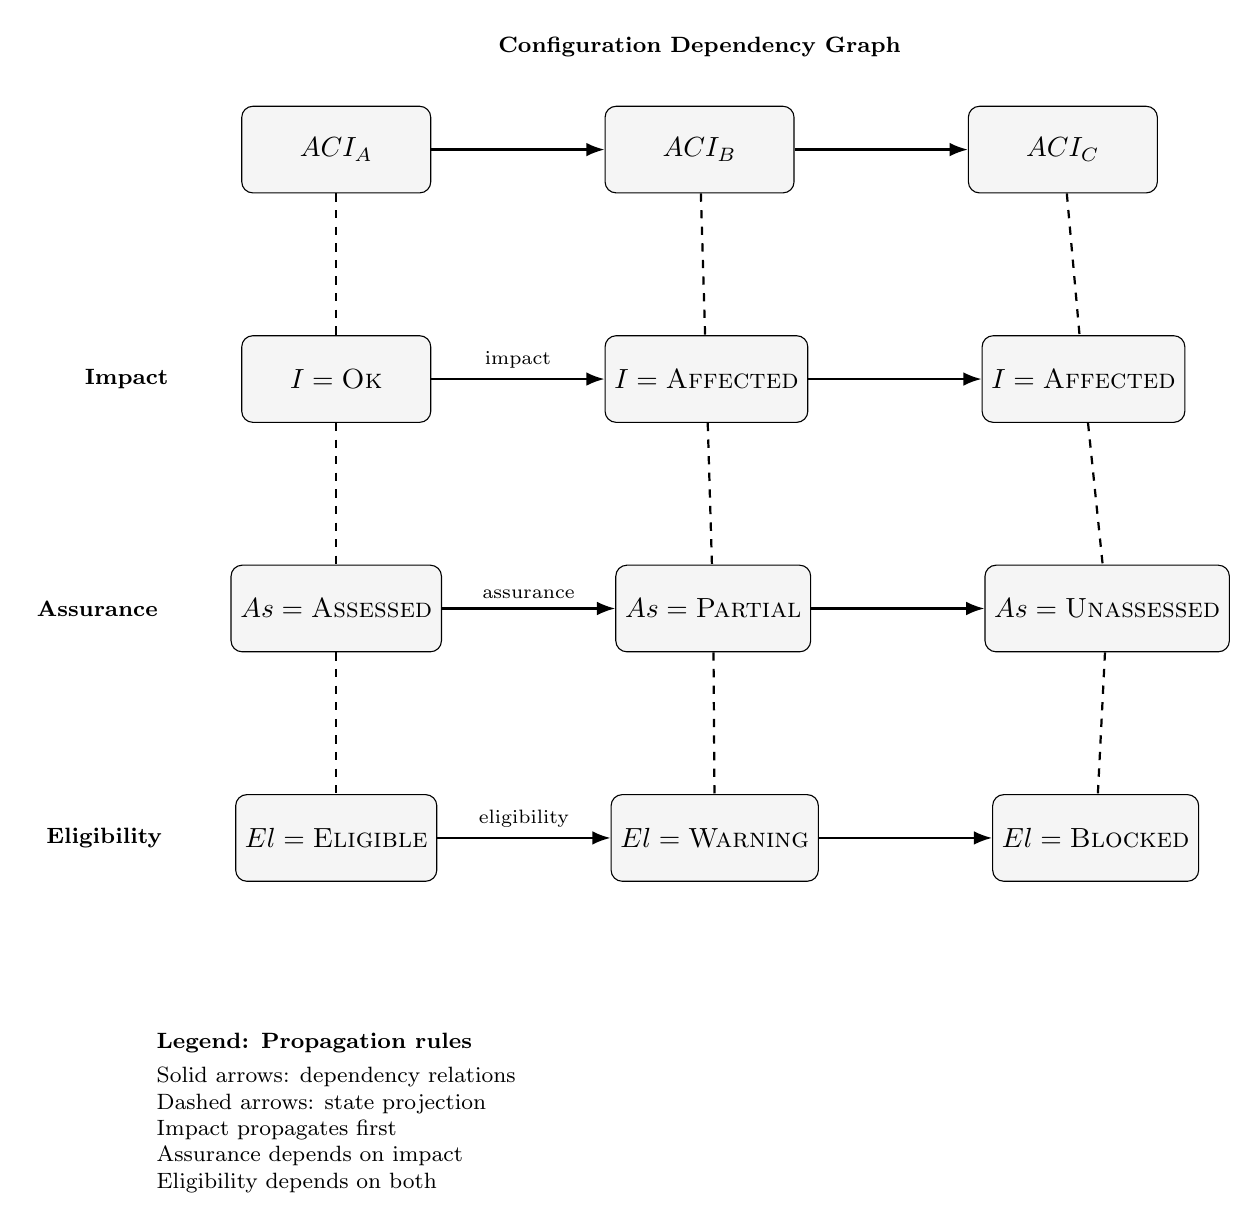
\begin{tikzpicture}[
    >=Latex,
    node distance=18mm and 22mm,
    aci/.style={
        draw,
        rounded corners,
        minimum width=24mm,
        minimum height=11mm,
        align=center,
        fill=gray!8
    },
    flow/.style={
        ->,
        thick
    },
    prop/.style={
        dashed,
        thick
    },
    annot/.style={
        font=\footnotesize,
        align=center
    }
]

%-------------------------------------------------
% Configuration graph
%-------------------------------------------------

\node[aci] (A) {$ACI_A$};
\node[aci,right=of A] (B) {$ACI_B$};
\node[aci,right=of B] (C) {$ACI_C$};

\draw[flow] (A)--(B);
\draw[flow] (B)--(C);

\node[annot,above=5mm of B]
{\textbf{Configuration Dependency Graph}};

%-------------------------------------------------
% Impact propagation
%-------------------------------------------------

\node[aci,below=18mm of A] (IA) {$I=\textsc{Ok}$};
\node[aci,right=of IA] (IB) {$I=\textsc{Affected}$};
\node[aci,right=of IB] (IC) {$I=\textsc{Affected}$};

\draw[prop] (A)--(IA);
\draw[prop] (B)--(IB);
\draw[prop] (C)--(IC);

\draw[flow] (IA)--node[above,font=\scriptsize]{impact}(IB);
\draw[flow] (IB)--node[above,font=\scriptsize]{}(IC);

\node[annot,left=8mm of IA]
{\textbf{Impact}};

%-------------------------------------------------
% Assurance propagation
%-------------------------------------------------

\node[aci,below=18mm of IA] (AA) {$As=\textsc{Assessed}$};
\node[aci,right=of AA] (AB) {$As=\textsc{Partial}$};
\node[aci,right=of AB] (AC) {$As=\textsc{Unassessed}$};

\draw[prop] (IA)--(AA);
\draw[prop] (IB)--(AB);
\draw[prop] (IC)--(AC);

\draw[flow] (AA)--node[above,font=\scriptsize]{assurance}(AB);
\draw[flow] (AB)--(AC);

\node[annot,left=8mm of AA]
{\textbf{Assurance}};

%-------------------------------------------------
% Eligibility propagation
%-------------------------------------------------

\node[aci,below=18mm of AA] (EA) {$El=\textsc{Eligible}$};
\node[aci,right=of EA] (EB) {$El=\textsc{Warning}$};
\node[aci,right=of EB] (EC) {$El=\textsc{Blocked}$};

\draw[prop] (AA)--(EA);
\draw[prop] (AB)--(EB);
\draw[prop] (AC)--(EC);

\draw[flow] (EA)--node[above,font=\scriptsize]{eligibility}(EB);
\draw[flow] (EB)--(EC);

\node[annot,left=8mm of EA]
{\textbf{Eligibility}};

%-------------------------------------------------
% Legend
%-------------------------------------------------

\node[
align=left,
below=18mm of EA,
font=\footnotesize
]
{
\textbf{Legend: Propagation rules}\\[1mm]
Solid arrows: dependency relations\\
Dashed arrows: state projection\\
Impact propagates first\\
Assurance depends on impact\\
Eligibility depends on both
};

\end{tikzpicture}

\caption{Governance state propagation across the configuration graph.
A structural dependency first propagates impact, which subsequently influences
assurance evaluation and finally execution eligibility. The three governance
dimensions remain conceptually independent while being evaluated in a
deterministic order.}
\label{fig:governance_propagation}
\end{figure}
%%%%%%%%%%%%%%%%%%%%%%%%%%%%%%%%%%%%%%%%%%%%%%%%%%%%%%%%%%%%%%%%%%%%%%%%%%%%%%%%

%%%%%%%%%%%%%%%%%%%%%%%%%%%%%%%%%%%%%%%%%%%%%%%%%%%%%%%%%%%%%%%%%%%%%%%%%%%%%%%%
\subsection{Runtime Semantics}
\label{subsec:runtime_semantics}

The governance semantics introduced in the previous sections describe the
evolution of immutable configuration revisions and their derived governance
states. Runtime semantics complement this model by defining how execution
observations are represented, normalized, and associated with governed
configuration items without modifying the underlying configuration baseline.

A fundamental design principle of ACM is the strict separation between
\emph{configuration state} and \emph{execution state}. The configuration graph describes the intended structure of an agentic system, whereas the runtime graph captures its actual execution. Runtime semantics define how execution events are represented, how runtime entities evolve throughout their execution, and how the observed execution can be reconciled with the governed configuration.

Each runtime entity is uniquely associated with the ACI revision from which it originates. This association preserves the complete traceability between the deployed configuration and the observed execution, allowing every runtime event to be interpreted in the context of the exact configuration revision that produced it. Runtime information therefore complements the immutable configuration model without modifying it.

During execution, runtime entities evolve according to a well-defined execution lifecycle. ACM distinguishes the states \textit{Created}, \textit{Running}, \textit{Completed}, \textit{Failed}, and \textit{Cancelled}. These states describe the operational progress of runtime instances independently of the governance lifecycle associated with their defining ACI revisions. Runtime transitions are event-driven and reflect the observed execution rather than governance decisions.

Runtime events record the significant occurrences affecting an executing system, including the creation of runtime instances, state transitions, delegated executions, tool invocations, dynamic artifact creation, and execution termination. Each event is timestamped and linked to the corresponding runtime entity, preserving both execution chronology and causal relationships between interacting components.

The runtime graph is progressively reconstructed from this event stream. Runtime relationships such as delegation, composition, or communication are therefore derived from observed execution rather than inferred from the static configuration graph. This distinction enables ACM to represent dynamic execution structures while maintaining a clear separation between declared configurations and runtime behavior.

The event log is append-only and preserves the chronological sequence of observed events. Because events are immutable and explicitly linked to their originating configuration revisions, the runtime graph can be deterministically reconstructed from the recorded execution history. Replay therefore provides a reproducible representation of the governed execution independently of the underlying orchestration framework.

Runtime semantics also support governance activities beyond execution monitoring. By comparing the reconstructed runtime graph with the approved configuration graph, ACM can identify undeclared runtime artifacts, unexpected dependency relationships, unauthorized executions, or deviations from the released baseline. These observations provide the information required for subsequent conformance assessment, drift analysis, and governance reporting.

The runtime model deliberately records observable governance events rather than implementation-specific execution details. As a result, heterogeneous orchestration frameworks can be represented through a common runtime representation while preserving the information necessary for traceability, reproducibility, and governance analysis. The complete formal semantics of runtime events, transition rules, replay, and graph reconstruction are provided in Appendix ~\ref{appendix:runtime_semantics}.


%%%%%%%%%%%%%%%%%%%%%%%%%%%%%%%%%%%%%%%%%%%%%%%%%%%%%%%%%%%%%%%%%%%%%%%%%%%%%%%%
\subsubsection{Framework-independent Runtime Normalization}

Native agentic frameworks expose heterogeneous execution models, event
structures, and tracing mechanisms. ACM deliberately avoids embedding any
framework-specific semantics within its governance kernel.

Instead, every framework is connected through a projection adapter that maps
native execution concepts onto the canonical runtime model defined above.

This separation satisfies the framework-independence principle introduced in
Section~\ref{sec:design_principles} and allows heterogeneous systems to be
evaluated using identical governance semantics.

Consequently, runtime conformance, assurance propagation, impact analysis,
and execution eligibility remain independent of the execution framework that
produced the observations.

%%%%%%%%%%%%%%%%%%%%%%%%%%%%%%%%%%%%%%%%%%%%%%%%%%%%%%%%%%%%%%%%%%%%%%%%%%%%%%%%
\subsubsection{Runtime Invariants}

The runtime semantics satisfy the following invariants.

\paragraph{Invariant R1 (Immutable Event History).}

Runtime events are append-only and cannot be modified once recorded.

\paragraph{Invariant R2 (Deterministic Reconstruction).}

Given an identical configuration baseline and an identical normalized event
sequence, replay reconstructs the same runtime graph.

\paragraph{Invariant R3 (Configuration Traceability).}

Every declared runtime entity shall be traceable to exactly one immutable
configuration revision through the projection function $\pi_r$, except for
undeclared runtime extensions explicitly represented by $\pi_r=\bot$.

These invariants provide the foundation upon which the dynamic-agent
governance semantics introduced in the next subsection are built.

%%%%%%%%%%%%%%%%%%%%%%%%%%%%%%%%%%%%%%%%%%%%%%%%%%%%%%%%%%%%%%%%%%%%%%%%%%%%%%%%
\subsection{Dynamic Agent Semantics}
\label{subsec:dynamic_agents}

Modern agentic systems frequently create agents during execution through delegation, planning, task decomposition, or adaptive workflows. ACM distinguishes these runtime-created agents from the immutable agent definitions that compose a released baseline. This distinction preserves the integrity of the governed configuration while allowing the runtime graph to evolve dynamically.

Every dynamic agent is represented as a runtime instance linked to its originating definition or to an approved \textit{AgentFactoryDefinition}. At creation time, the runtime instance records its creator, the execution context, the resolved configuration, the effective prompts, models, tools, policies, permissions, and a configuration digest. These attributes ensure that dynamically generated agents remain fully traceable and reproducible within the execution history.

Agent factories define the governance constraints under which dynamic agents may be created. They specify the templates that may be instantiated, the attributes that may be overridden, the authorized models and tools, permission ceilings, delegation limits, runtime lifetime, and any additional constraints required by the governing policy. Dynamic agent creation is therefore governed by explicit policies rather than unrestricted runtime behavior.

A fundamental governance rule is that dynamic agents cannot obtain capabilities exceeding those granted by their creator or authorized by the corresponding factory. Attempts to introduce unauthorized models, tools, policies, permissions, or other forbidden overrides violate the applicable governance policy and produce a \textit{blocked} eligibility state. This conservative approach ensures that runtime adaptation never bypasses configuration governance.

Dynamic agents also follow a dedicated promotion lifecycle that is independent of the governance lifecycle of ordinary ACI revisions. Newly created runtime objects are initially considered transient execution artifacts. They may subsequently be retained for analysis, proposed for reuse, and eventually promoted into ordinary configuration items through the standard governance process. Promotion never modifies the released baseline that originated the execution. Instead, it creates a new immutable ACI revision subject to the same governance, assurance, and lifecycle requirements as any other managed configuration item.

By separating immutable definitions from runtime instances and by governing their promotion explicitly, ACM enables controlled runtime adaptation while preserving configuration integrity, complete traceability, and reproducible governance decisions. The complete promotion lifecycle, transition rules, and validation constraints are provided in Appendix ~\ref{appendix:dynamic_agent}.

%%%%%%%%%%%%%%%%%%%%%%%%%%%%%%%%%%%%%%%%%%%%%%%%%%%%%%%%%%%%%%%%%%%%%%%%%%%%%%%%
\subsubsection{Configuration Overrides}

Runtime adaptation frequently requires modifying selected configuration
attributes of a dynamically instantiated agent.

Examples include:

\begin{itemize}
\item prompt parameter substitution;
\item execution context injection;
\item temporary memory allocation;
\item execution metadata.
\end{itemize}

ACM models these modifications as runtime overrides rather than configuration
changes.Each override is evaluated against the governance policy attached to the
corresponding agent definition. Overrides therefore modify only runtime behaviour without altering the
immutable configuration revision.

%%%%%%%%%%%%%%%%%%%%%%%%%%%%%%%%%%%%%%%%%%%%%%%%%%%%%%%%%%%%%%%%%%%%%%%%%%%%%%%%
\subsubsection{Governance Constraints}

Every runtime agent inherits the governance constraints attached to its parent
definition.

These constraints include:

\begin{itemize}
\item authorized tools;
\item permitted models;
\item execution policies;
\item security permissions;
\item assurance requirements.
\end{itemize}

Consequently, runtime flexibility never bypasses governance decisions already
attached to the originating configuration revision.

Whenever an override violates one of these constraints, the corresponding
runtime instance becomes non-compliant.

Such violations are propagated through the governance semantics introduced in
Sections~\ref{subsec:assurance_semantics} and
\ref{subsec:governance_state_propagation}.


%%%%%%%%%%%%%%%%%%%%%%%%%%%%%%%%%%%%%%%%%%%%%%%%%%%%%%%%%%%%%%%%%%%%%%%%%%%%%%%%
\subsubsection{Discussion}

The proposed semantics deliberately separate immutable agent definitions from
their runtime realizations. This distinction allows ACM to support highly
dynamic execution models while preserving configuration immutability,
deterministic governance evaluation, and complete execution traceability.

Consequently, dynamic agent creation becomes a runtime concern rather than a
configuration-management concern, thereby preserving the framework-independent
nature of the ACM reference model.

%%%%%%%%%%%%%%%%%%%%%%%%%%%%%%%%%%%%%%%%%%%%%%%%%%%%%%%%%%%%%%%%%%%%%%%%%%%%%%%%
\subsection{Governance Semantics Summary}
\label{subsec:governance_summary}

This section established the formal governance semantics that constitute the
normative core of the ACM reference model. While the preceding sections defined
the structural representation of Agentic Configuration Items (ACIs), the
governance semantics specify how these immutable configuration artifacts evolve,
interact and constrain execution throughout the lifecycle of an agentic system.

The proposed semantics rely on a clear separation between immutable
configuration revisions and derived governance states. Lifecycle states,
quality, assurance, impact and execution eligibility are intentionally modeled
as orthogonal dimensions, each governed by its own semantic rules and
transition mechanisms. This separation prevents changes affecting one
governance dimension from implicitly modifying the others, thereby improving
traceability, explainability and reproducibility. The Table ~\ref{tab:semantic_space_state} summarizes the different space states associated to governance lifecycle, governance quality, assurance, impact and eligibility.

\begin{table}[t]
	\caption{XX}
	\label{tab:semantic_space_state}
	\centering
	\begin{tabular}{ll}
		\hline
		Dimension & States\\
		\hline
		 & \\
		Governance Lifecyle & $Draft, Review, Validated, Approved, Deprecated,  Archived$ \\
		 & \\
		Governance Quality State & $Undefined, Valid, Warning, Invalid$ \\
		 & \\
		Impact State   & $None, Local, Propagated$ \\
		 & \\
		Assurance State   & $Unassessed, Partial, Satisfied$ \\
		 & \\
		Eligibility State  & $Eligible, Restricted, Blocked$ \\
		 & \\
		\hline
	\end{tabular}
\end{table}

A second fundamental principle introduced in this section is the distinction
between configuration semantics and runtime semantics. Immutable configuration
graphs describe the intended structure of an agentic system, whereas runtime
graphs capture execution observations without altering published baselines.
Dynamic agents, runtime events and execution traces are therefore treated as
governed runtime entities whose provenance remains continuously linked to the
configuration revisions from which they originate.

The governance semantics further define deterministic propagation rules for
impact, assurance and execution eligibility. Rather than propagating lifecycle
states directly, ACM propagates governance consequences according to explicit
dependency policies. This approach preserves the intrinsic properties of
configuration revisions while enabling accurate impact analysis and governance
evaluation across complex dependency graphs.

Together, these semantics establish a framework-independent governance model
capable of representing both static configurations and dynamic execution
behaviour within a unified formal framework. The resulting model remains
independent of any particular orchestration framework, execution engine or
runtime implementation while providing a deterministic basis for governance
evaluation, reproducibility and auditability.

The following section demonstrates how these formal semantics can be
operationalized through a reference implementation. The implementation should
not be interpreted as an extension of the model itself, but rather as an
executable instantiation showing that the proposed governance semantics can be
implemented consistently and applied to heterogeneous agentic frameworks while
preserving the properties established throughout this section.

\section{Operationalization}
\label{sec:operationalization}

The purpose of this section is not to define another execution framework but to demonstrate that the proposed reference model is operationalizable without introducing framework-specific concepts into its governance semantics. The operationalization deliberately separates governance semantics from implementation details. The ACM metamodel, lifecycle semantics, and validation rules are independent of programming language, persistence technology, communication protocol, or execution framework. The Python implementation therefore serves only as one concrete realization of the reference model, demonstrating implementability rather than prescribing a specific software architecture. The experimental methodology is depicted in Figure ~\ref{fig:experimental_protocol}.

\begin{figure*}[t]
	\centering
	
\includegraphics[width=0.5\textwidth]{figures/experimental_protocol.png}
	\caption{Overview of the experimental methodology. Native framework configurations are projected into the ACM reference model through semantic projection, validated using normative governance scenarios and automated invariant checking, and finally evaluated with respect to model expressiveness, semantic preservation, and framework independence.}
	\label{fig:experimental_protocol}
\end{figure*}

\subsection{Reference Architecture}
\label{subsec:reference_architecture}
As mentioned earlier, the ACM reference model is intentionally independent of any particular agentic framework. Its operationalization therefore relies on a layered architecture that separates framework-specific extraction from framework-independent governance. This separation preserves the conceptual independence of the reference model while enabling heterogeneous agentic systems to be represented through a common governed configuration.

Figure~\ref{fig:acm_reference_architecture} illustrates the reference architecture adopted by the ACM reference implementation. The operationalization process consists of five successive stages that progressively transform a native agentic system into a governed ACM representation.

%%%%%%%%%%%%%%%%%%%%%%%%%%%%%%%%%%%%%%%%%%%%%%%%%%%%%%%%%%%%%%%%%%%%%%%%%%%%%%%%
% Required packages and libraries
%
% \usepackage{tikz}
% \usetikzlibrary{
%     arrows.meta,
%     positioning,
%     fit,
%     backgrounds,
%     calc
% }
%%%%%%%%%%%%%%%%%%%%%%%%%%%%%%%%%%%%%%%%%%%%%%%%%%%%%%%%%%%%%%%%%%%%%%%%%%%%%%%%

\begin{figure}[t]
\centering

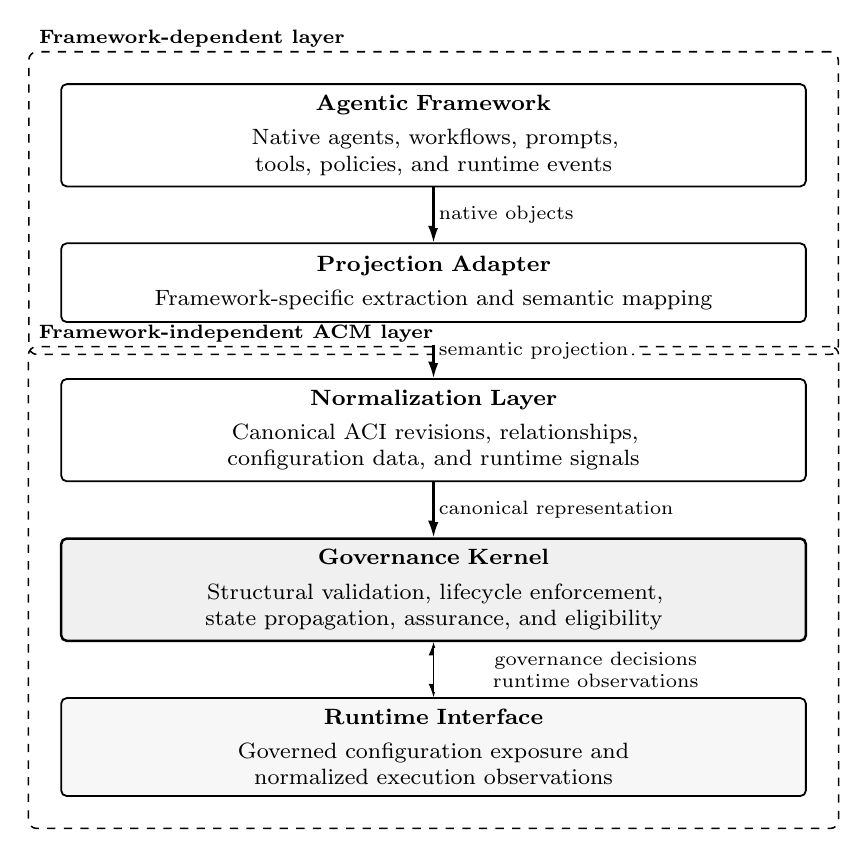
\begin{tikzpicture}[
    font=\footnotesize,
    >=Latex,
    node distance=7mm,
    stage/.style={
        draw,
        rounded corners=2pt,
        minimum width=0.78\columnwidth,
        minimum height=10mm,
        text width=0.68\columnwidth,
        align=center,
        line width=0.65pt,
        fill=white,
        inner sep=4pt
    },
    kernel/.style={
        stage,
        line width=0.9pt,
        fill=gray!12
    },
    runtime/.style={
        stage,
        fill=gray!6
    },
    flow/.style={
        -{Latex[length=2.1mm,width=1.4mm]},
        line width=0.8pt
    },
    bidirectional/.style={
        {Latex[length=2mm,width=1.3mm]}-
        {Latex[length=2mm,width=1.3mm]},
        line width=0.8pt
    },
    edgeLabel/.style={
        font=\scriptsize,
        fill=white,
        inner sep=1.5pt,
        align=center
    },
    boundary/.style={
        draw,
        dashed,
        rounded corners=3pt,
        line width=0.55pt,
        inner sep=4mm
    },
    boundaryLabel/.style={
        font=\scriptsize\bfseries,
        fill=white,
        inner sep=1pt
    }
]

%------------------------------------------------------------------------------
% Main processing pipeline
%------------------------------------------------------------------------------

\node[stage] (framework) {
    \textbf{Agentic Framework}\\[1mm]
    Native agents, workflows, prompts, tools,
    policies, and runtime events
};

\node[stage, below=of framework] (adapter) {
    \textbf{Projection Adapter}\\[1mm]
    Framework-specific extraction and semantic mapping
};

\node[stage, below=of adapter] (normalization) {
    \textbf{Normalization Layer}\\[1mm]
    Canonical ACI revisions, relationships,
    configuration data, and runtime signals
};

\node[kernel, below=of normalization] (governance) {
    \textbf{Governance Kernel}\\[1mm]
    Structural validation, lifecycle enforcement,
    state propagation, assurance, and eligibility
};

\node[runtime, below=of governance] (runtime) {
    \textbf{Runtime Interface}\\[1mm]
    Governed configuration exposure and
    normalized execution observations
};

%------------------------------------------------------------------------------
% Directed processing flow
%------------------------------------------------------------------------------

\draw[flow]
    (framework.south)
    --
    node[edgeLabel, right]
    {native objects}
    (adapter.north);

\draw[flow]
    (adapter.south)
    --
    node[edgeLabel, right]
    {semantic projection}
    (normalization.north);

\draw[flow]
    (normalization.south)
    --
    node[edgeLabel, right]
    {canonical representation}
    (governance.north);

%------------------------------------------------------------------------------
% Bidirectional runtime interaction
%------------------------------------------------------------------------------

\draw[<->]
    (governance.south)
    --
    node[edgeLabel, right, text width=40mm]
    {governance decisions\\
     runtime observations}
    (runtime.north);

%------------------------------------------------------------------------------
% Responsibility boundaries
% These elements are placed behind the main nodes.
%------------------------------------------------------------------------------

\begin{scope}[on background layer]

    \node[
        boundary,
        fit=(framework)(adapter)
    ] (frameworkBoundary) {};

    \node[
        boundary,
        fit=(normalization)(governance)(runtime)
    ] (acmBoundary) {};

\end{scope}

%------------------------------------------------------------------------------
% Boundary labels
%------------------------------------------------------------------------------

\node[
    boundaryLabel,
    anchor=south west
] at ($(frameworkBoundary.north west)+(1mm,0)$)
{
    Framework-dependent layer
};

\node[
    boundaryLabel,
    anchor=south west
] at ($(acmBoundary.north west)+(1mm,0)$)
{
    Framework-independent ACM layer
};

\end{tikzpicture}

\caption{Reference architecture for the operationalization of ACM. Native
framework constructs are extracted through framework-specific projection
adapters and translated into canonical representations before entering the
framework-independent governance kernel. The runtime interface exposes
governance decisions and returns normalized execution observations without
modifying immutable configuration revisions.}
\label{fig:acm_reference_architecture}

\end{figure}

The reference implementation should not be interpreted as a production platform or a preferred execution environment. Its primary purpose is to demonstrate that the ACM reference model is sufficiently precise to support deterministic validation, semantic projection, and reproducible governance across heterogeneous agentic frameworks. Alternative implementations could realize the same governance semantics while adopting different architectures, storage technologies, or execution environments. Our implementation is supported by the following elements of architecture:

\begin{enumerate}
    \item \textbf{Framework Extraction} retrieves the native configuration artifacts exposed by an execution framework. These artifacts include configuration objects, metadata, structural relationships, and execution-specific information without modifying their original semantics.

    \item \textbf{Semantic Projection} translates the extracted artifacts into ACM concepts through framework-specific projection rules. Rather than reproducing the native representation verbatim, this stage reconstructs an equivalent governance-oriented representation preserving the semantics required by the ACM reference model.

    \item \textbf{ACM Normalization} converts the projected artifacts into canonical ACM objects. This process assigns stable identities, creates immutable Agentic Configuration Item (ACI) revisions, resolves references, computes canonical digests, and constructs the logical configuration graphs introduced in Section~\ref{sec:reference_model}.

    \item \textbf{Governance Processing} applies the formal governance semantics defined in Section~\ref{sec:governance_semantics}. Validation, lifecycle management, assurance computation, state propagation, and runtime integration are all performed exclusively on normalized ACM objects, independently of the originating framework.

    \item \textbf{Governed Representation} produces a complete ACM configuration composed of immutable revisions, governed relationships, baselines, runtime information, and provenance metadata. This representation becomes the unique input for validation, auditing, replay, and lifecycle management.
\end{enumerate}

The resulting architecture deliberately isolates framework-specific concerns from governance concerns. Native frameworks remain responsible for execution, while ACM provides a unified configuration representation upon which governance operations can be performed consistently across heterogeneous ecosystems.

%%%%%%%%%%%%%%%%%%%%%%%%%%%%%%%%%%%%%%%%%%%%%%%%%%%%%%%%%%%%%%%%%%%%%%%%%%%%%%%%
\subsection{Projection Pipeline}
\label{subsec:semantic_projection_pipeline}

The reference architecture introduced in
Section~\ref{subsec:reference_architecture} separates framework-specific
extraction from framework-independent governance evaluation. This separation is
implemented through a semantic projection pipeline that transforms native
framework structures into the canonical representation defined by the ACM
reference model.

The objective of this pipeline is not to reproduce the complete internal
execution model of each framework. Instead, it identifies the subset of native
constructs that carry configuration or governance significance and maps them
onto Agentic Configuration Items (ACIs), typed relationships, immutable
revisions, and normalized runtime observations.

The projection pipeline comprises four successive stages:

\begin{enumerate}
    \item native structure extraction;
    \item semantic classification;
    \item canonical normalization;
    \item projection validation and coverage assessment.
\end{enumerate}

The semantic projection pipeline is detailed in Appendix ~\ref{appendix:projection_formalism}


%%%%%%%%%%%%%%%%%%%%%%%%%%%%%%%%%%%%%%%%%%%%%%%%%%%%%%%%%%%%%%%%%%%%%%%%%%%%%%%%
\subsubsection{Framework-specific Instantiations}

The prototype operationalizes this pipeline through dedicated adapters for
LangGraph and CrewAI. Each adapter applies the same canonical projection
contract while preserving framework-specific extraction logic.

For both frameworks, the evaluation reports:

\begin{itemize}
    \item the number of governance-relevant native entities;
    \item the number of completely, partially, and unsuccessfully projected
    entities;
    \item the number of governance-relevant native relationships;
    \item the corresponding entity, relationship, aggregate, and strict
    coverage scores.
\end{itemize}

The measured values are presented in
Section~\ref{sec:evaluation}. They are intentionally not inferred from the
existence of a functioning adapter: they are computed from the explicit
construct inventory defined by the evaluation protocol.

This distinction is essential for Research Question~1. A successful execution
of the projection pipeline demonstrates technical feasibility, whereas
Projection Coverage measures the expressiveness of the ACM reference model with
respect to the evaluated framework constructs.

\subsection{Framework Adapters}
\label{sec:framework_adapters}

The semantic projection pipeline is instantiated through framework-specific adapters responsible for extracting native configuration artifacts and translating them into ACM representations. Although each adapter is tailored to the internal abstractions of a particular framework, all of them produce the same normalized ACM representation described in the previous section.

The central objective of the operationalization through adapters is therefore not to reproduce the native execution semantics of individual frameworks, but to project their configuration artifacts into a common governance representation while preserving the information required for lifecycle management, provenance, dependency analysis, and assurance. This distinction enables heterogeneous frameworks to be represented through a common configuration model while isolating framework-specific concerns within the projection layer.

To illustrate this approach, the reference implementation currently provides adapters for two agentic frameworks exhibiting markedly different orchestration paradigms: LangGraph and CrewAI.

Table~\ref{tab:framework_mapping} summarizes the principal conceptual correspondences established by the LangGraph and CrewAI adapters.

\begin{table}[ht]
\centering
\caption{Representative LangGraph and CrewAI to ACM Concept Mapping}
\label{tab:langgraph_mapping}
\begin{tabular}{lll}
	\toprule
	\textbf{ACM} & \textbf{LangGraph} & \textbf{CrewAI} \\
	\midrule
	Workflow Definition & Graph & Crew \\
	Agent Definition & Node &  Agent \\
	Structural Relationships & Edge &  Flow\\
	Tool Definition & Tool & Tool \\
	Prompt Definition & Prompt & Prompt\\
	Runtime State & State & -- \\
	Workflow Node & -- & Task \\
	Runtime Events & Execution Events & Runtime Events \\
	\bottomrule
\end{tabular}
\end{table}


\subsubsection{LangGraph Projection}

LangGraph represents agentic systems as explicit stateful execution graphs composed of interconnected nodes, conditional transitions, shared state, and tool invocations. Because the execution topology is explicitly materialized by the framework, most structural relationships can be projected directly into the ACM Configuration Graph.

The LangGraph adapter traverses the native graph definition and extracts the configuration artifacts required by the ACM reference model. Agent definitions, prompts, tools, workflow topology, and associated metadata are translated into immutable Agentic Configuration Items (ACIs), while graph edges are converted into structural relationships preserving execution dependencies.

Since LangGraph exposes an explicit workflow structure, semantic reconstruction remains limited. Most governance information required by ACM is already available through the native graph description, allowing the projection process to preserve both structural relationships and configuration provenance with minimal interpretation.

Runtime events generated during execution are normalized through the ACM Runtime Graph without modifying the underlying execution semantics. Consequently, lifecycle management, assurance computation, and governance state propagation operate on a representation that remains independent of LangGraph while preserving the information required for configuration governance.


\subsubsection{CrewAI Projection}

CrewAI adopts a substantially different orchestration paradigm based on cooperating agents, tasks, crews, and flows rather than on an explicit execution graph. Consequently, part of the structural organization required by ACM is not directly represented by native framework objects and must be reconstructed during semantic projection.

The CrewAI adapter extracts the declarative configuration describing crews, agents, tasks, tools, prompts, and execution flows before translating these elements into ACM configuration artifacts. While individual configuration objects can generally be mapped directly to corresponding ACI types, the workflow topology often requires semantic reconstruction from the relationships implicitly expressed by task assignments, execution dependencies, and flow definitions.

This reconstruction does not attempt to reproduce CrewAI's internal implementation mechanisms. Instead, it identifies the governance-relevant relationships necessary to construct an equivalent Configuration Graph preserving configuration provenance, dependency analysis, lifecycle management, and runtime traceability.

Following normalization, CrewAI configurations become indistinguishable from configurations originating from other supported frameworks. All subsequent governance algorithms therefore operate on a unified ACM representation without requiring framework-specific processing.



\subsubsection{Comparative Analysis}

The two adapters illustrate complementary projection scenarios representative of current agentic ecosystems. LangGraph exposes an explicit execution graph, allowing a largely structural projection, whereas CrewAI relies on higher-level declarative abstractions requiring additional semantic reconstruction.

Despite these architectural differences, both adapters produce equivalent ACM representations composed of immutable configuration items, normalized relationships, governed baselines, runtime events, and provenance metadata. Consequently, all governance algorithms described in the following sections operate without any knowledge of the originating framework.

This result supports one of the central design principles of ACM: governance mechanisms should depend exclusively on the normalized configuration representation rather than on framework-specific execution models. Framework adapters therefore constitute the only framework-dependent component of the operationalization, while the governance kernel remains entirely framework-independent.

\subsection{Governance Processing}
\label{sec:governance_algorithms}

Once a native configuration has been transformed into a normalized ACM representation, governance becomes entirely independent of the originating framework. All subsequent processing stages operate exclusively on immutable ACM artifacts and therefore share the same behavior regardless of whether the configuration originates from LangGraph, CrewAI, or any future supported framework.

Rather than introducing new algorithms, the reference implementation organizes governance processing as a deterministic sequence of four processing stages. Each stage operates on the output of the previous one while preserving the framework-independent semantics defined in Section~\ref{sec:governance_semantics}. Figure~\ref{fig:governance_processing_pipeline} summarizes this workflow.

\begin{figure}[ht]
\centering
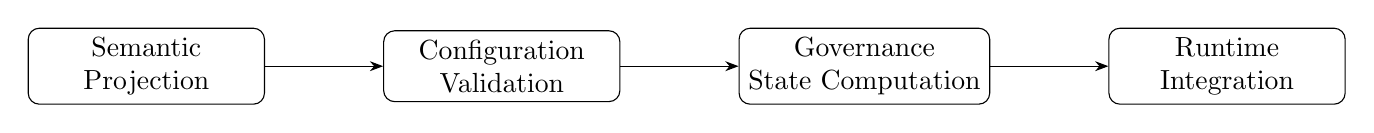
\begin{tikzpicture}[
node distance=1.5cm,
every node/.style={
draw,
rounded corners,
align=center,
minimum width=3cm,
minimum height=0.8cm
},
>=Stealth
]

\node (projection) {Semantic\\Projection};
\node (validation) [right=of projection] {Configuration\\Validation};
\node (states) [right=of validation] {Governance\\State Computation};
\node (runtime) [right=of states] {Runtime\\Integration};

\draw[->] (projection) -- (validation);
\draw[->] (validation) -- (states);
\draw[->] (states) -- (runtime);

\end{tikzpicture}

\caption{Governance processing pipeline implemented by the reference operationalization.}
\label{fig:governance_processing_pipeline}
\end{figure}

\subsubsection{Processing Stage 1: Semantic Projection}

The first processing stage transforms framework-specific configuration artifacts into ACM concepts according to the semantic projection rules introduced in Section~\ref{sec:semantic_projection}. The objective is to preserve governance-relevant semantics rather than reproduce the native internal representation of the originating framework.

\begin{algorithm}[ht]
\caption{Semantic Projection}
\KwIn{Native framework configuration $F$}
\KwOut{Projected ACM objects}

Extract native artifacts\;

Apply framework-specific projection rules\;

Create projected ACM objects\;

Preserve provenance metadata\;

\Return projected configuration\;

\end{algorithm}

The resulting representation remains independent of governance processing and serves as the input to the normalization and validation stages.

\subsubsection{Processing Stage 2: Configuration Validation}

Configuration validation verifies that the projected ACM representation satisfies the structural constraints required by the reference model before governance states are computed.

Validation is intentionally deterministic and independent of runtime execution. It verifies object identities, reference consistency, relationship integrity, digest computation, and structural constraints while preserving the immutability of validated revisions.

\begin{algorithm}[ht]
\caption{Configuration Validation}
\KwIn{Normalized ACM configuration}
\KwOut{Validated configuration}

Resolve references\;

Verify structural constraints\;

Compute canonical digests\;

Detect structural inconsistencies\;

Produce validation report\;

\Return validated configuration\;

\end{algorithm}

Only validated ACM representations are processed by the governance engine.

\subsubsection{Processing Stage 3: Governance State Computation}

Once the configuration has been validated, governance states are computed according to the formal semantics introduced in Section~\ref{sec:governance_semantics}. This stage evaluates lifecycle status, impact propagation, eligibility, and assurance until a deterministic fixed point is reached.

Unlike lifecycle states, which remain intrinsic properties of immutable revisions, computed governance states are derived from the dependency structure of the configuration graph and may therefore evolve whenever dependencies change.

\begin{algorithm}[ht]
\caption{Governance State Computation}
\KwIn{Validated ACM configuration}
\KwOut{Computed governance states}

Initialize computed states\;

Repeat

\Indp

Compute impact propagation\;

Update eligibility\;

Update assurance\;

\Indm

Until convergence\;

\Return governed configuration\;

\end{algorithm}

Because propagation is deterministic over a finite configuration graph, convergence always produces a unique governance state for a given configuration and governance policy.

\subsubsection{Processing Stage 4: Runtime Integration}

The final processing stage incorporates runtime observations into the governance model without modifying immutable configuration artifacts. Runtime signals are normalized into ACM runtime events and integrated into the Runtime Graph introduced in Section~\ref{sec:governance_semantics}.

This separation preserves the distinction between governed configurations and operational execution while enabling replay, auditing, and runtime traceability.

\begin{algorithm}[ht]
\caption{Runtime Integration}
\KwIn{Runtime events}
\KwOut{Updated Runtime Graph}

Normalize runtime events\;

Update runtime graph\;

Maintain provenance\;

Enable replay reconstruction\;

\Return runtime representation\;

\end{algorithm}

Since runtime integration operates exclusively on normalized events, the resulting Runtime Graph remains independent of the native event formats exposed by individual execution frameworks.

\subsection{Reference Implementation}
\label{sec:reference_implementation}

The ACM reference model is operationalized through an open-source Python reference implementation developed to validate the feasibility of the proposed concepts and governance semantics. The implementation is intentionally presented as a reference operationalization rather than as a production-ready governance platform. Its primary objective is to demonstrate that the reference model can be realized using deterministic processing stages while remaining independent of any particular execution framework.

The implementation follows the layered architecture introduced in Section~\ref{sec:operationalization}. Framework-specific adapters are responsible for semantic projection, whereas the governance kernel operates exclusively on normalized ACM representations. This architectural separation ensures that governance algorithms remain independent of framework-specific execution models and may therefore be reused by future adapters without modification.

The implementation organizes configuration artifacts as immutable Agentic Configuration Item (ACI) revisions represented through strongly typed data models. Canonical serialization and content-addressed digests provide stable identities for configuration revisions, enabling deterministic comparison, provenance tracking, baseline management, and reproducible replay of governed configurations.

Governance processing is implemented as a deterministic pipeline corresponding directly to the formal semantics introduced in Section~\ref{sec:governance_semantics}. Configuration validation, lifecycle management, governance state computation, and runtime integration operate on immutable configuration revisions without modifying the underlying configuration artifacts. Runtime observations are maintained separately within the Runtime Graph, preserving the conceptual distinction between governed configurations and operational execution.

The modular organization of the reference implementation also facilitates extensibility. Supporting an additional agentic framework only requires the implementation of a new semantic projection adapter capable of producing normalized ACM artifacts. Since all subsequent governance processing operates exclusively on the normalized representation, no modification of the governance kernel is required when integrating additional frameworks (see Figure ~\ref{fig:operationalization_acm}).

\begin{figure*}[t]
	\centering
	
\includegraphics[width=\textwidth]{figures/operationalization_acm.png}
	\caption{Operationalization of the ACM reference model through semantic projection. Native framework configurations are projected into a common framework-independent governance representation, while a reference implementation demonstrates validation, runtime replay and conformance, and impact analysis based on the ACM governance semantics.}
	\label{fig:operationalization_acm}
\end{figure*}

Thus, the reference implementation serves as the experimental artifact supporting the evaluation presented in Section~\ref{sec:evaluation}. All normative scenarios, automated validation procedures, and cross-framework projection experiments reported in this paper are executed using this implementation, providing empirical evidence that the ACM reference model can be operationalized consistently while preserving framework-independent governance semantics. Finally, operationalization validates the implementability of the reference model; evaluation validates its expressiveness.

\begin{table}[ht]
\centering
\caption{Correspondence between ACM concepts and the reference implementation.}
\label{tab:implementation_mapping}
\begin{tabular}{ll}
\toprule
\textbf{ACM Concept} & \textbf{Reference Implementation} \\
\midrule
Reference Model & Strongly typed ACI data models \\
Semantic Projection & Framework adapters \\
Governance Processing & Deterministic governance kernel \\
Configuration Graphs & Canonical graph representations \\
Runtime Semantics & Runtime event normalization \\
Reference Operationalization & Python implementation \\
\bottomrule
\end{tabular}
\end{table}

The Figure ~\ref{fig:aci_metamodel_implementation} depicts the UML representation of an ACI object in the reference implementation.

\begin{figure*}[t]
	\centering
	
\includegraphics[width=\textwidth]{figures/ACI_metamodel.png}
	\caption{UML representation of the core ACIRevision model in the ACM reference implementation. The diagram shows the immutable ACIRevision object together with its references, declared governance state, assurance policy, and associated enumerations, providing the structural basis of the reference implementation.}
	\label{fig:aci_metamodel_implementation}
\end{figure*}

\section{Evaluation}
\label{sec:evaluation}

The previous section demonstrated how the ACM reference model can be operationalized through a framework-independent governance architecture, semantic projection pipeline, and reference implementation. The remaining question is whether this operationalization effectively preserves the governance semantics defined by the reference model while supporting heterogeneous agentic frameworks in practice.

The objective of this evaluation is therefore not to benchmark execution performance or compare orchestration frameworks. Instead, it assesses the extent to which the ACM reference model provides a consistent and operational foundation for configuration governance across heterogeneous agentic systems. More specifically, the evaluation investigates whether configurations originating from different frameworks can be projected into a common representation while preserving governance-relevant semantics and enabling deterministic governance processing.

The evaluation is conducted using the Python reference implementation presented in Section~\ref{sec:operationalization}. Two representative agentic frameworks, LangGraph and CrewAI, are used as experimental case studies because they embody distinct orchestration paradigms while remaining sufficiently mature and widely adopted within the current agentic ecosystem. The experimental protocol combines semantic projection experiments, normative governance scenarios, automated validation procedures, and runtime integration experiments in order to assess the operational feasibility of the proposed reference model.

The remainder of this section is organized as follows. Section~7.1 introduces the research questions guiding the evaluation. Section~7.2 describes the experimental methodology. Section~7.3 presents the experimental results, while Section~7.4 discusses their implications with respect to the objectives of the ACM reference model.

\subsection{Evaluation Objectives}
\label{sec:evaluation_objectives}

The evaluation aims to determine whether the ACM reference model fulfills the objectives defined throughout this paper. Rather than evaluating implementation-specific characteristics, the experiments focus on validating the conceptual properties of the reference model, its governance semantics, and its ability to provide a common governance layer across heterogeneous agentic frameworks.

To structure the evaluation, four research questions are defined.

\begin{itemize}

\item \textbf{RQ1 -- Expressiveness.}
Can the ACM reference model represent heterogeneous agentic configurations originating from different orchestration frameworks using a common governance representation?

\item \textbf{RQ2 -- Governance Preservation.}
Does semantic projection preserve the governance-relevant semantics of native configurations, including configuration identity, provenance, dependency relationships, lifecycle information, and runtime traceability?

\item \textbf{RQ3 -- Operational Feasibility.}
Can the governance semantics introduced in this paper be operationalized through a deterministic processing pipeline supporting configuration validation, governance state computation, and runtime integration?

\item \textbf{RQ4 -- Framework Independence.}
Can identical governance mechanisms be applied to configurations originating from structurally different frameworks without modifying the governance kernel?

\end{itemize}

These research questions directly reflect the principal design objectives introduced in Sections~3--6. Consequently, the evaluation does not attempt to compare the execution capabilities of individual agentic frameworks. Instead, it investigates whether ACM succeeds in abstracting framework-specific configuration models into a unified governance representation while preserving the semantics required for configuration management.

The following sections describe the experimental methodology adopted to answer these research questions and present the empirical evidence collected using the reference implementation.

\begin{table}[ht]
\centering
\caption{Research questions and evaluation criteria.}
\label{tab:research_questions}
\begin{tabular}{p{1cm} p{4.6cm} p{5.8cm}}
\toprule
\textbf{RQ} & \textbf{Objective} & \textbf{Evaluation Evidence} \\
\midrule
RQ1 & Assess the expressiveness of the ACM representation & Cross-framework semantic projection \\
RQ2 & Assess governance semantics preservation & Projection outcome analysis and governance validation \\
RQ3 & Assess operational feasibility & Automated governance scenarios and deterministic processing \\
RQ4 & Assess framework independence & Cross-framework execution of identical governance mechanisms \\
\bottomrule
\end{tabular}
\end{table}
\subsection{Experimental Methodology}
\label{sec:evaluation_methodology}

The experimental methodology was designed to evaluate the ACM reference model with respect to the research questions introduced in Section~\ref{sec:evaluation_objectives}. Rather than measuring execution performance, the experiments assess whether heterogeneous agentic configurations can be governed through a common configuration model while preserving the governance semantics defined throughout this paper.

All experiments were conducted using the Python reference implementation described in Section~\ref{sec:reference_implementation}. This implementation realizes the semantic projection pipeline, governance processing stages, and runtime integration mechanisms introduced in Section~\ref{sec:operationalization}. It serves exclusively as an experimental artifact supporting the evaluation of the reference model.

Two representative agentic frameworks were selected as experimental case studies:

\begin{itemize}
\item \textbf{LangGraph}, representing explicit graph-based orchestration;
\item \textbf{CrewAI}, representing declarative agent-task orchestration.
\end{itemize}

These frameworks were intentionally chosen because they rely on different orchestration abstractions while exposing sufficiently rich configuration models to evaluate the framework-independence of ACM.

The evaluation combines four complementary experimental activities:

\begin{enumerate}

\item semantic projection of native framework configurations into normalized ACM representations;

\item execution of normative governance scenarios covering lifecycle management, dependency propagation, assurance evaluation, and runtime semantics;

\item automated validation of governance invariants and deterministic processing through the reference implementation;

\item comparative analysis of governance behavior across both frameworks.

\end{enumerate}

This methodology provides complementary evidence regarding both the conceptual validity of the ACM reference model and its practical operationalization. While semantic projection evaluates the expressiveness of the reference model, the governance scenarios validate the formal semantics introduced in Section~\ref{sec:governance_semantics}. Automated validation ensures that governance processing remains deterministic and reproducible, whereas the comparative analysis assesses the framework independence of the proposed governance architecture.

\begin{table}[ht]
\centering
\caption{Experimental protocol used to evaluate the ACM reference model.}
\label{tab:experimental_protocol}

\begin{tabular}{p{3.8cm}p{3.8cm}p{4.4cm}}
\toprule
\textbf{Experimental Activity} &
\textbf{Objective} &
\textbf{Research Questions} \\
\midrule

Semantic Projection &
Evaluate representational expressiveness &
RQ1, RQ2 \\

Governance Scenarios &
Validate governance semantics &
RQ2, RQ3 \\

Automated Validation &
Verify deterministic governance processing &
RQ3 \\

Cross-framework Comparison &
Assess framework independence &
RQ1, RQ4 \\

\bottomrule
\end{tabular}

\end{table}

\begin{figure}[ht]
\centering

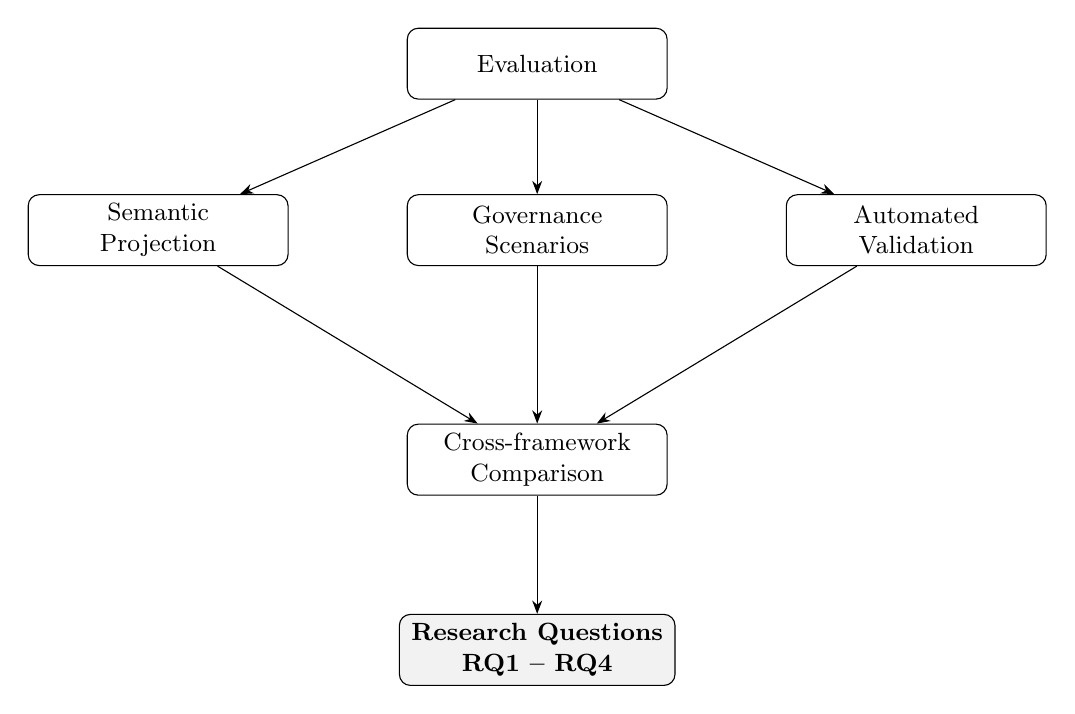
\begin{tikzpicture}[
node distance=1.2cm and 1.5cm,
>=Stealth,
process/.style={
draw,
rounded corners,
align=center,
minimum width=3.3cm,
minimum height=0.9cm,
font=\small
},
rq/.style={
draw,
rounded corners,
fill=gray!10,
align=center,
minimum width=3.5cm,
minimum height=0.9cm,
font=\small\bfseries
}
]

% Top
\node[process] (eval) {Evaluation};

% Middle row
\node[process, below left=of eval] (projection) {Semantic\\Projection};

\node[process, below=of eval] (scenarios) {Governance\\Scenarios};

\node[process, below right=of eval] (validation) {Automated\\Validation};

% Comparison
\node[process, below=2.0cm of scenarios] (comparison)
{Cross-framework\\Comparison};

% Bottom
\node[rq, below=1.5cm of comparison]
(rqs)
{Research Questions\\RQ1 -- RQ4};

% Connections
\draw[->] (eval) -- (projection);
\draw[->] (eval) -- (scenarios);
\draw[->] (eval) -- (validation);

\draw[->] (projection) -- (comparison);
\draw[->] (scenarios) -- (comparison);
\draw[->] (validation) -- (comparison);

\draw[->] (comparison) -- (rqs);

\end{tikzpicture}

\caption{Experimental methodology adopted to evaluate the ACM reference model. Complementary experimental activities collectively provide evidence for answering the research questions.}

\label{fig:evaluation_methodology}

\end{figure}

\subsection{Evaluation Results}
\label{sec:experimental_results}

This section presents the experimental evidence collected using the methodology described in Section~\ref{sec:experimental_methodology}. The objective is not to evaluate execution performance, but to assess whether the ACM reference model satisfies the research questions introduced in Section~\ref{sec:evaluation_objectives}. The reported results are derived from the latest validation and preservation reports generated by the reference implementation.

The evaluation addresses four complementary dimensions: (i) the representational expressiveness of ACM, (ii) the preservation of governance semantics during semantic projection, (iii) the deterministic operationalization of the governance model, and (iv) the framework-independent behavior of the governance kernel.

%%%%%%%%%%%%%%%%%%%%%%%%%%%%%%%%%%%%%%%%%%%%%%%%%%%%%%%%%%%%%%%%%%%%%%%%%%%%%%%%
\subsubsection{Model Expressiveness}
\label{subsubsec:model_expressiveness}

The first research question investigates whether ACM provides a sufficiently
expressive configuration model to represent heterogeneous agentic systems while
preserving the governance information required for lifecycle management,
traceability, and runtime conformance.

Unlike programming languages, where expressiveness is often associated with the
set of computable behaviors, the notion of expressiveness considered in this
work refers to the ability of the reference model to faithfully represent the
configuration semantics of an existing agentic framework.

Accordingly, the expressiveness of ACM is operationalized through three
complementary dimensions:

\begin{enumerate}
	\item \textbf{Configuration Coverage}, measuring how many native
	configuration constructs can be represented by ACM;
	\item \textbf{Semantic Preservation}, measuring whether the governance
	meaning of supported constructs is preserved after projection;
	\item \textbf{Information Loss}, measuring the proportion of native
	information that cannot be represented by the current reference
	model.
\end{enumerate}

These dimensions provide a quantitative characterization of expressiveness that
can be reproduced independently of the implementation (see Appendix ~\ref{appendix:evaluation_semantics}). The related Research Questions and their evaluation are presented in Table ~\ref{tab:evaluation_metrics}.

\begin{table}[t]
	\centering
	\caption{Relationship between evaluation metrics and experimental evidence.}
	\label{tab:evaluation_metrics}
	\renewcommand{\arraystretch}{1.2}
	\begin{tabularx}{\linewidth}{lXX}
		\toprule
		\textbf{Metric} &
		\textbf{Primary Evaluation Method} &
		\textbf{Purpose} \\
		\midrule
		
		Configuration Coverage &
		Semantic projection experiments (LangGraph and CrewAI) &
		Assess whether governance-relevant native constructs can be represented by the ACM reference model. \\
		
		Semantic Preservation (Expressiveness) &
		Preservation analysis and normative scenarios &
		Assess whether the governance semantics of projected configurations are preserved and satisfy the expected ACM invariants. \\
		
		Information Loss &
		Preservation reports generated during semantic projection &
		Identify and characterize governance-relevant information that cannot currently be represented or must be approximated by the reference model. \\
		
		\bottomrule
	\end{tabularx}
\end{table}

\paragraph{Overall Expressiveness}

The three previous metrics characterize complementary aspects of model
expressiveness.

Configuration Coverage evaluates representational completeness, Semantic
Preservation evaluates governance fidelity, and Information Loss quantifies the
remaining limitations of the current reference model.

Rather than combining these dimensions into a single weighted score, they are
reported independently throughout the evaluation. This choice preserves their
interpretability and avoids introducing arbitrary weighting factors that would
depend on the characteristics of individual frameworks.


\subsubsection{Governance Semantics Preservation}

A principal objective of semantic projection is the preservation of governance-relevant semantics rather than the exact reproduction of native framework implementations.

According to the preservation reports, both evaluated adapters preserve all structural elements within the normative ACM scope. Nodes, structural relationships, workflow branches, entry points, terminal nodes, prompt references, tool references, and canonical configuration digests are preserved for the evaluated workflows. Repeated projections produce identical canonical digests, demonstrating deterministic normalization.

The only remaining approximations concern execution semantics that are intentionally opaque to the native frameworks themselves. In particular, conditional routing logic implemented through arbitrary Python functions cannot be reconstructed statically and is therefore represented as an abstract routing structure. Likewise, CrewAI Flow state schemas currently remain outside the normative ACM scope and are consequently classified as unsupported rather than reconstructed.

Importantly, these limitations affect execution-specific implementation details rather than the governance semantics required by ACM. Configuration identity, provenance, dependency relationships, lifecycle information, runtime traceability, and configuration validation remain fully preserved throughout the projection process.

\begin{table}[ht]
\centering
\caption{Governance semantics preservation for the evaluated workflows.}
\label{tab:preservation_summary}

\begin{tabular}{lccc}
\toprule
\textbf{Governance Property} &
\textbf{Preserved} &
\textbf{Approximated} &
\textbf{Unsupported} \\
\midrule
Configuration identity & \checkmark & - & - \\
Revision provenance & \checkmark & - & - \\
Dependency graph & \checkmark & - & - \\
Prompt references & \checkmark & - & - \\
Tool references & \checkmark & - & - \\
Canonical digests & \checkmark & - & - \\
Conditional routing semantics & - & \checkmark & - \\
Framework-specific runtime state & - & - & \checkmark \\
\bottomrule
\end{tabular}

\end{table}

%%%%%%%%%%%%%%%%%%%%%%%%%%%%%%%%%%%%%%%%%%%%%%%%%%%%%%%%%%%%%%%%%%%%%%%%%%%%%%%%
\subsubsection{Operational Results}
\label{subsubsec:operational_results}

The reference implementation was evaluated using the complete experimental
protocol described previously. The evaluation combined declarative fixtures,
dedicated scenario-specific tests, framework adapters, runtime validation, and
benchmark experiments (Complete scenarios description in Appendix ~\ref{appendix:configuration_baseline}).

Overall, the evaluation successfully completed the complete normative scenario
suite without unresolved implementation inconsistencies after the final
refinements of the governance kernel. The resulting experimental campaign
covered all fourteen normative invariants introduced in
Section~\ref{sec:governance_semantics} and exercised the principal governance
mechanisms of the reference model.

Table~\ref{tab:scenario_results} summarizes the execution results obtained for
the twenty-seven evaluation scenarios.

\begin{table}[t]
\caption{Summary of operational evaluation results.}
\label{tab:scenario_results}
\centering
\begin{tabular}{lc}
\hline
Metric & Result\\
\hline
Normative scenarios & 27\\
Declarative fixtures & 11\\
Normative invariants evaluated & 14\\
Automated tests passed & 221\\
Automated tests skipped & 3\\
Kernel inconsistencies requiring refinement & 2\\
\hline
\end{tabular}
\end{table}

Beyond the numerical results, the evaluation provides several observations that
directly address the research questions introduced in
Section~\ref{sec:evaluation_methodology}.

\paragraph{Contribution to RQ1 (Model Expressiveness).}

These results provide positive evidence for \textbf{RQ1}. They show that ACM is sufficiently expressive to capture the governance-relevant configuration concepts of the evaluated agentic systems while preserving the information required for lifecycle management, dependency modeling, provenance, runtime traceability, and governance evaluation. Importantly, framework-specific constructs that cannot yet be represented are explicitly reported during semantic projection rather than silently discarded, making the current boundaries of the reference model transparent and enabling controlled future extensions.

\paragraph{Contribution to RQ2 (Semantic Preservation).}

These results provide positive evidence for \textbf{RQ2}. They indicate that the governance semantics defined by ACM are preserved throughout the semantic projection process (defined in
Section~\ref{sec:governance_semantics} and in Appendix ~\ref{appendix:projection_formalism}) including lifecycle transitions, dependency propagation, assurance evaluation, eligibility computation, runtime traceability, and drift detection. The deterministic replay experiments further demonstrate that governance states can be reconstructed reproducibly from normalized runtime events independently of probabilistic LLM outputs. The discrepancies initially identified in scenarios ACM-S02 and ACM-S20 led to normative refinements of the reference implementation, illustrating the effectiveness of the scenario-based validation methodology in strengthening the consistency between the formal specification and its operational realization.

\paragraph{Contribution to RQ3 (Framework Independence).}

These results provide positive evidence for \textbf{RQ3}. They demonstrate that governance-relevant configurations originating from structurally different orchestration frameworks can be projected into a common ACM representation while preserving the governance semantics required for lifecycle management, provenance, dependency analysis, and runtime governance. The consistent behavior of semantic projection and runtime normalization across the evaluated scenarios further supports the framework-independent design objective of ACM. These findings should nevertheless be interpreted within the scope of the present study: they demonstrate the feasibility of normalizing representative configurations from two complementary orchestration paradigms rather than universal compatibility with all existing or future agentic frameworks.

\paragraph{Overall Interpretation.}

Taken together, the operational results indicate that the reference
implementation faithfully operationalizes the proposed governance semantics and
that the experimental protocol is sufficiently comprehensive to evaluate the
principal properties of the ACM reference model. Rather than merely
demonstrating software correctness, the evaluation provides empirical evidence
that the concepts introduced by ACM are internally consistent, reproducible,
and applicable across heterogeneous agentic configurations within the scope of
the evaluated frameworks.

%%%%%%%%%%%%%%%%%%%%%%%%%%%%%%%%%%%%%%%%%%%%%%%%%%%%%%%%%%%%%%%%%%%%%%%%%%%%%%%%
\subsection{Discussion of Results}
\label{subsec:discussion_results}

The experimental evaluation provides evidence that the proposed ACM reference
model constitutes a coherent governance abstraction for agentic systems. Beyond
the individual research questions addressed in the previous subsections, several
broader observations emerge from the evaluation.

First, the scenario-based validation demonstrates that governance can be
specified independently of execution frameworks. Throughout the experimental
campaign, the same governance semantics were successfully applied to different
orchestration paradigms after semantic projection into the ACM reference model.
This separation between implementation-specific execution and
framework-independent governance is one of the principal architectural
contributions of ACM.

Second, the evaluation confirms the importance of treating configuration as an
immutable governance artifact rather than as a mutable runtime object.
Lifecycle transitions, assurance propagation, dependency analysis, runtime
traceability, and deterministic replay all rely on immutable revisions whose
identities remain stable throughout the system lifecycle. This design enables
governance decisions to be reproduced and audited independently of the
probabilistic behavior of the underlying language models.

Third, the experimental campaign illustrates the value of formal governance
semantics. Rather than serving solely as theoretical specifications, the
normative invariants provided an executable contract against which the reference
implementation could be continuously validated. The two implementation
discrepancies identified during the evaluation (ACM-S02 and ACM-S20) were not
limitations of the methodology but evidence of its effectiveness in revealing
ambiguities requiring refinement of the governance kernel. The final model
therefore benefits directly from the iterative interaction between formal
specification and implementation.

The evaluation highlights the current scope of ACM. The experiments
demonstrate that the proposed governance semantics are applicable across the
representative orchestration frameworks considered in this work while remaining
computationally practical for the evaluated configuration sizes. At the same
time, the study intentionally does not claim universal framework compatibility
or enterprise-scale validation. These aspects constitute natural directions for
future extensions of the reference model.

Overall, the results support the central hypothesis of this work: governance of
agentic systems can be modeled independently from execution frameworks through
an immutable configuration model, explicit lifecycle semantics, deterministic
governance propagation, and runtime traceability. The consistency observed
across the complete evaluation campaign suggests that ACM provides a sound
foundation upon which richer governance capabilities can be developed in future
work.

\begin{table}[ht]

\centering

\caption{Summary of research question outcomes.}

\label{tab:rq_summary}

\begin{tabular}{p{1cm}p{2.7cm}p{5cm}p{2cm}}

\toprule

\textbf{RQ} &
\textbf{Objective} &
\textbf{Evidence} &
\textbf{Outcome}

\\

\midrule

RQ1 &
Expressiveness &
Successful cross-framework representation &
Supported

\\

RQ2 &
Governance preservation &
Semantic preservation analysis &
Supported

\\

RQ3 &
Operational feasibility &
Automated validation and deterministic processing &
Supported

\\

RQ4 &
Framework independence &
Identical governance processing across frameworks &
Supported within evaluated scope

\\

\bottomrule

\end{tabular}

\end{table}

\section{Discussion}
\label{sec:discussion}
\subsection{Positioning with Respect to Existing Agentic Frameworks}
\label{sec:positioning}

The rapid emergence of agentic frameworks has significantly simplified the development of LLM-based applications by providing increasingly sophisticated abstractions for workflow orchestration, agent coordination, tool integration, and execution management. Frameworks such as LangGraph and CrewAI exemplify this evolution by exposing distinct orchestration paradigms tailored to different classes of agentic systems.

The objective of ACM is fundamentally different. Rather than providing execution capabilities, ACM introduces a framework-independent governance layer dedicated to the management of agentic configurations throughout their lifecycle. Consequently, ACM should not be interpreted as an alternative orchestration framework, but as a complementary governance model capable of operating across heterogeneous execution environments.

This distinction is reflected in the responsibilities addressed by each approach. Agentic frameworks primarily define how agents execute, communicate, and coordinate during runtime. ACM, by contrast, governs what is being executed by providing immutable configuration revisions, provenance tracking, lifecycle management, dependency analysis, baseline management, assurance evaluation, and runtime traceability. Execution and governance therefore constitute complementary concerns operating at different abstraction levels.

The semantic projection mechanism provides the interface between these two layers (see Appendix ~\ref{appendix:projection_formalism}). By translating framework-specific configurations into normalized ACM artifacts, governance processing becomes independent of the originating execution framework while preserving the governance semantics required for configuration management. This separation allows identical governance mechanisms to be applied to configurations originating from heterogeneous orchestration paradigms without introducing framework-specific logic into the governance kernel.

More generally, the proposed architecture aligns with the long-established separation between execution infrastructures and configuration management observed in traditional software engineering. Source code management systems, build systems, deployment platforms, and runtime environments have historically evolved as complementary but distinct components of the software lifecycle \cite{ref25}. ACM extends this principle to agentic systems by introducing an explicit governance layer dedicated to the management of agentic configurations rather than their execution.

The experimental evaluation presented in Section~\ref{sec:evaluation} provides initial evidence supporting this positioning. The successful projection of representative LangGraph and CrewAI workflows into a common ACM representation demonstrates that governance can be decoupled from execution while preserving the semantics required for configuration management. Although the current evaluation remains limited to two representative frameworks, the obtained results suggest that this architectural separation provides a viable foundation for framework-independent governance of agentic systems.

\begin{figure}[t]
    \centering

    \begin{tikzpicture}[
        font=\scriptsize,
        node distance=4mm and 3mm,
        layer/.style={
            draw,
            rounded corners=1.5pt,
            minimum width=0.94\columnwidth,
            inner xsep=4pt,
            inner ysep=5pt,
            align=center,
            line width=0.6pt
        },
        component/.style={
            draw,
            rounded corners=1pt,
            minimum height=6mm,
            inner xsep=4pt,
            inner ysep=2pt,
            align=center,
            line width=0.45pt
        },
        projection/.style={
            draw,
            minimum width=0.58\columnwidth,
            minimum height=6mm,
            align=center,
            line width=0.6pt
        },
        arrow/.style={
            -{Latex[length=2mm,width=1.3mm]},
            line width=0.65pt
        }
    ]

    % ---------------------------------------------------------
    % Execution layer
    % ---------------------------------------------------------

    \node[layer] (execution) {
        \textbf{Agentic Execution Frameworks}\\[4pt]
        \begin{tikzpicture}[
            baseline,
            component/.style={
                draw,
                rounded corners=1pt,
                minimum width=21mm,
                minimum height=6mm,
                align=center,
                line width=0.45pt
            }
        ]
            \node[component] (langgraph) {LangGraph};
            \node[component, right=2mm of langgraph] (crewai) {CrewAI};
            \node[component, right=2mm of crewai] (others) {Other Frameworks};
        \end{tikzpicture}
    };

    % ---------------------------------------------------------
    % Semantic projection
    % ---------------------------------------------------------

    \node[projection, below=5mm of execution] (projection) {
        \textbf{Semantic Projection}\\
        Framework-specific adapter and normalization
    };

    \draw[arrow] (execution) -- (projection);

    % ---------------------------------------------------------
    % ACM governance layer
    % ---------------------------------------------------------

    \node[layer, below=5mm of projection] (acm) {
        \textbf{ACM Framework-Independent Governance Layer}\\[4pt]
        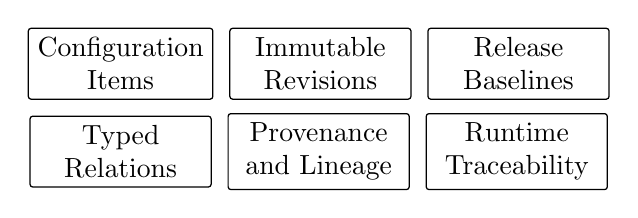
\begin{tikzpicture}[
            baseline,
            component/.style={
                draw,
                rounded corners=1pt,
                minimum width=23mm,
                minimum height=6mm,
                align=center,
                line width=0.45pt
            }
        ]
            \node[component] (aci) {Configuration\\Items};
            \node[component, right=2mm of aci] (revisions) {Immutable\\Revisions};
            \node[component, right=2mm of revisions] (baselines) {Release\\Baselines};

            \node[component, below=2mm of aci] (relations) {Typed\\Relations};
            \node[component, right=2mm of relations] (provenance) {Provenance\\and Lineage};
            \node[component, right=2mm of provenance] (runtime) {Runtime\\Traceability};
        \end{tikzpicture}
    };

    \draw[arrow] (projection) -- (acm);

    % ---------------------------------------------------------
    % Governance capabilities
    % ---------------------------------------------------------

    \node[layer, below=5mm of acm] (governance) {
        \textbf{Governance Capabilities}\\[4pt]
        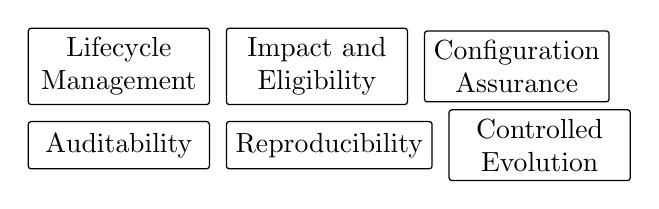
\begin{tikzpicture}[
            baseline,
            component/.style={
                draw,
                rounded corners=1pt,
                minimum width=23mm,
                minimum height=6mm,
                align=center,
                line width=0.45pt
            }
        ]
            \node[component] (lifecycle) {Lifecycle\\Management};
            \node[component, right=2mm of lifecycle] (impact) {Impact and\\Eligibility};
            \node[component, right=2mm of impact] (assurance) {Configuration\\Assurance};

            \node[component, below=2mm of lifecycle] (audit) {Auditability};
            \node[component, right=2mm of audit] (reproducibility) {Reproducibility};
            \node[component, right=2mm of reproducibility] (change) {Controlled\\Evolution};
        \end{tikzpicture}
    };

    \draw[arrow] (acm) -- (governance);

    \end{tikzpicture}

    \caption{Positioning of ACM with respect to agentic execution frameworks. Framework-specific configurations are semantically projected into a common governance representation, allowing lifecycle, assurance, traceability, and change-management mechanisms to operate independently of the originating framework.}
    \label{fig:acm_framework_positioning}
\end{figure}

\subsection{Contributions to Agentic Configuration Governance}
\label{sec:governance_contributions}

The contribution of ACM lies neither in introducing a new orchestration mechanism nor in extending the execution capabilities of existing agentic frameworks. Its primary contribution is to establish configuration governance as an explicit and framework-independent concern for agentic systems. From this perspective, ACM contributes at four complementary levels: representation, semantics, interoperability, and operational validation.

\subsubsection{A Framework-Independent Governance Representation}

The first contribution is a reference model that represents an agentic system as a governed configuration rather than as a collection of framework-specific runtime objects. The model introduces explicit configuration items, immutable revisions, typed relationships, provenance information, and release baselines. These abstractions provide a common vocabulary for describing the constituent elements of an agentic system and the dependencies that determine its effective configuration.

This representation extends established configuration-management principles to artifacts that are specific to agentic systems. In particular, it treats agents, prompts, tools, policies, models, workflows, and dynamically instantiated components as governable objects whose identity and evolution can be tracked independently. The resulting configuration is therefore not reduced to source code, deployment metadata, or execution traces. It is represented as an explicit and auditable object in its own right.

A central consequence of this model is the ability to distinguish logical identity from immutable revision identity. Successive revisions of the same configuration item preserve a stable conceptual identity while remaining individually addressable through exact revision identifiers and content digests. This distinction supports reproducibility, comparison, controlled replacement, and historical reconstruction without conflating an evolving artifact with one of its concrete states.

\subsubsection{Formal Governance Semantics}

The second contribution is the formalization of governance semantics over the reference model. ACM does not merely describe which artifacts exist; it defines how their governance states evolve and how local changes affect dependent configurations.

The lifecycle model specifies admissible transitions for configuration revisions, baselines, and runtime instances. Quality, assurance, impact, and eligibility are maintained as distinct dimensions rather than being collapsed into a single status. This separation prevents ambiguous interpretations such as treating a lack of evidence as proof of poor quality or propagating the lifecycle state of a dependency directly to its parent.

The propagation semantics further define how dependency changes, invalidated evidence, deprecated components, and runtime deviations influence the governance status of composite configurations. These effects are restrictive rather than destructive: a problematic dependency may block the promotion of a composite configuration without rewriting the intrinsic quality or lifecycle state of that composite. The model thereby preserves the provenance of governance decisions while supporting deterministic and explainable state computation.

The assurance model complements these semantics by linking governance conclusions to explicit evidence. Validation and approval are attached to exact revisions and scopes, allowing the system to distinguish directly assessed artifacts from conclusions inherited through assurance-relevant dependencies. Governance states can therefore be interpreted together with the evidence and rules from which they were derived.

\subsubsection{Framework-Independent Semantic Projection}

The third contribution is the separation between framework-specific extraction and framework-independent governance processing. Native configurations are translated into ACM through semantic projection, while the governance kernel operates exclusively on normalized ACM artifacts.

This architecture allows heterogeneous orchestration paradigms to be governed through a common representation. A graph-oriented framework may expose nodes and edges directly, whereas a role- and task-oriented framework may require part of its topology to be reconstructed from assignments and dependencies. ACM does not require these native representations to be structurally identical. It requires the projection to preserve the information needed for configuration governance and to make approximated or unavailable information explicit.

Framework independence should therefore be understood as independence of the governance model and processing semantics from a specific execution framework. The adapters remain framework-specific because they interpret native concepts. Once projection is complete, however, lifecycle validation, baseline construction, dependency analysis, assurance computation, runtime integration, and impact propagation no longer depend on the source framework.

This separation provides a basis for interoperability without imposing a common execution model. Frameworks retain their native orchestration semantics, while ACM supplies a shared governance representation above them.

\subsubsection{Reference Operationalization and Evaluation}

The fourth contribution is the operationalization of the reference model through an executable implementation and its evaluation across two distinct agentic frameworks. The Python prototype demonstrates that the proposed abstractions and semantics can be implemented as deterministic processing mechanisms rather than remaining solely conceptual definitions.

The reference implementation operationalizes immutable revisions, canonical serialization, configuration validation, state propagation, baseline processing, runtime-event normalization, and replay. The LangGraph and CrewAI adapters instantiate the semantic-projection boundary for two frameworks with different native abstractions. Their use does not establish universal applicability, but provides initial evidence that the model can accommodate both explicit graph structures and role--task compositions.

The evaluation also contributes a structured validation methodology combining normative governance scenarios, automated tests, and semantic-preservation analysis. This methodology distinguishes successful representation from exact structural equivalence and records which governance-relevant properties are preserved, reconstructed, approximated, or unavailable. It therefore provides a more appropriate validation criterion for a reference model than conventional runtime-performance benchmarking.

Taken together, these four contributions establish ACM as a configuration-governance abstraction positioned between agentic execution environments and higher-level operational or organizational governance processes. The reference model defines what is governed, the formal semantics define how governance states are computed, semantic projection connects heterogeneous frameworks to the model, and the reference implementation demonstrates that these mechanisms can be operationalized consistently.

\subsection{Practical Implications}
\label{sec:practical_implications}

Beyond its conceptual contribution, ACM has practical implications for the engineering and governance of agentic systems. By introducing an explicit and framework-independent configuration representation, the proposed model enables governance activities that are difficult to perform when configuration information remains fragmented across framework-specific abstractions.

A first implication concerns reproducibility. In current agentic ecosystems, reproducing a previous execution often requires reconstructing configurations from multiple heterogeneous artifacts, including prompts, workflow definitions, deployment parameters, runtime traces, and external resources. ACM addresses this fragmentation by associating executions with immutable configuration revisions and controlled release baselines. A governed execution can therefore be traced back to the exact configuration from which it originated, supporting reproducible experiments, regression analyses, and long-term maintenance.

A second implication concerns auditability and traceability. Since governance decisions are explicitly linked to identified configuration revisions and supporting evidence, the provenance of a validation result or lifecycle transition becomes inspectable rather than implicit. This capability facilitates post-deployment analysis, compliance reporting, and forensic investigation by making configuration evolution transparent throughout the lifecycle of the system.

The explicit representation of dependencies also supports systematic change management. Instead of reasoning independently about prompts, agents, tools, or models, ACM represents these artifacts as interconnected configuration items whose relationships can be analyzed before modifications are promoted to a released baseline. Dependency-aware impact analysis provides early visibility into the potential consequences of configuration changes, reducing the likelihood of unintended regressions.

The proposed model also provides a common governance abstraction that may facilitate interoperability across heterogeneous execution environments. Organizations frequently combine multiple orchestration frameworks to address different operational requirements. By projecting these heterogeneous configurations into a shared governance representation, ACM enables governance policies to be expressed independently of the underlying execution technology while allowing each framework to preserve its native execution semantics.

ACM may therefore contribute to the emerging AgentOps ecosystem by complementing existing observability and orchestration platforms with explicit configuration governance. Current operational platforms primarily focus on execution monitoring, tracing, evaluation, and operational metrics. ACM addresses a complementary concern by governing the configuration artifacts that determine how those executions are produced. Consequently, the model should be viewed as a governance layer that can coexist with, rather than replace, existing AgentOps and LLMOps infrastructures.

%%%%%%%%%%%%%%%%%%%%%%%%%%%%%%%%%%%%%%%%%%%%%%%%%%%%%%%%%%%%%%%%%%%%%%%%%%%%%%%%
\subsection{Limitations of the Current Reference Model}
\label{subsec:limitations}

The objective of ACM is to provide a framework-independent governance representation for the governance of agentic system configurations rather than an execution platform or an autonomous reasoning architecture. Accordingly, the current version focuses on representing governed configuration artifacts, their lifecycle, dependencies, provenance, assurance, and runtime conformance, while intentionally leaving the internal execution logic of agentic systems outside the scope of the reference model.

Table~\ref{tab:limitations_scope} summarizes the current coverage of ACM and the principal capabilities intentionally deferred to future work.

\begin{table}[t]
	\caption{Current scope of the ACM reference model.}
	\label{tab:limitations_scope}
	\centering
	\begin{tabular}{p{3.1cm}p{3.4cm}}
		\hline
		\textbf{Currently covered} &
		\textbf{Not yet covered} \\
		\hline
		Semantic projection &
		Distributed execution \\
		Configuration governance &
		Multi-agent planning strategies \\
		Immutable revision management &
		Learning and adaptation mechanisms \\
		Lifecycle semantics &
		Autonomous reasoning policies \\
		Dependency propagation &
		Self-modifying execution strategies \\
		Runtime provenance &
		Collective agent negotiation \\
		Assurance evaluation &
		Long-term memory management \\
		Deterministic replay &
		Continual learning \\
		\hline
	\end{tabular}
\end{table}

These limitations result from deliberate modeling decisions rather than technical constraints. ACM intentionally separates governance concerns from execution concerns in order to establish a stable and framework-independent governance layer. Integrating planning algorithms, reasoning strategies, learning mechanisms, or execution optimizations into the reference model would both increase its complexity and compromise the conceptual independence required for long-term interoperability.

Consequently, ACM treats reasoning engines, orchestration frameworks, planning modules, learning components, communication protocols, and other execution technologies as external systems whose observable configuration and runtime behavior can be represented and governed without prescribing their internal operation. ACM therefore specifies \emph{what} is governed---configuration revisions, baselines, dependencies, runtime observations, and assurance evidence---rather than \emph{how} autonomous agents reason, plan, negotiate, or learn.

This separation also preserves the stability of the governance model as agentic technologies evolve. New execution frameworks, orchestration paradigms, communication protocols, or reasoning techniques can be incorporated through semantic projection without modifying the governance semantics themselves. The evaluation presented in this paper should therefore be interpreted as validating the ability of ACM to represent and govern heterogeneous agentic configurations, not the correctness, efficiency, or intelligence of the underlying execution mechanisms.

The experimental validation remains limited to the representative orchestration frameworks and configuration scales considered by the reference implementation. Although the reported results provide encouraging evidence regarding the generality of the proposed governance semantics, additional empirical validation across larger industrial deployments, additional execution frameworks, and emerging agentic ecosystems will be required before broader generalization can be claimed.

\subsection{Section Summary}

This discussion has positioned ACM as a framework-independent governance representation dedicated to the governance of agentic system configurations. Rather than introducing a new execution framework, orchestration engine, or reasoning architecture, ACM provides a common semantic foundation for representing, governing, and auditing heterogeneous agentic configurations throughout their lifecycle.

The proposed reference model combines a unified configuration representation with formal governance semantics and a framework-independent operationalization. The evaluation demonstrates that these concepts can be instantiated consistently across structurally different agentic frameworks while preserving the governance information required for lifecycle management, provenance, assurance, runtime conformance, and reproducibility within the evaluated scope.

The discussion has also emphasized that ACM deliberately defines a minimal yet extensible governance core. Native execution abstractions—including framework-specific orchestration constructs, communication protocols, optimization mechanisms, and reusable skills—are treated as governed artifacts through semantic projection rather than as first-class governance concepts. This design preserves the stability and framework independence of the reference model while allowing it to accommodate the continuing evolution of agentic ecosystems without modifying its core governance semantics.

The following section examines the principal threats to the validity of this study and discusses the methodological and experimental factors that should be considered when interpreting the reported results.

\section{Threats to Validity}
\label{sec:threats_validity}

The preceding sections presented the ACM reference model, its formal governance semantics, its operationalization through a reference implementation, and an experimental evaluation conducted across two heterogeneous agentic frameworks. Together, these elements provide evidence that the proposed model is internally consistent, operationally realizable, and capable of preserving governance semantics within the evaluated scope.

As with any reference model, however, these results must be interpreted within the boundaries of the assumptions, implementation choices, and experimental conditions that characterize the present study. The purpose of this section is therefore not to question the conceptual validity of ACM itself, but to identify the principal factors that may influence the interpretation, reproducibility, and generalization of the reported results.

Following established empirical research practice, we distinguish threats related to the scope of the reference model, the validation of its formal semantics, the internal validity of the experimental methodology, the external validity of the reported conclusions, and the reproducibility of the evaluation artifacts. These limitations define the current scope of evidence supporting ACM and naturally motivate the research directions discussed in the following section.

\subsection{Validity of the Reference Model}
\label{sec:validity_reference_model}

The primary objective of this study is to evaluate whether ACM provides a sufficiently expressive and framework-independent governance representation for representing and governing heterogeneous agentic system configurations. Consequently, the reported results should be interpreted as evidence supporting the proposed reference model within the scope of the evaluated frameworks rather than as a demonstration of universal applicability.

The evaluation intentionally considers two agentic frameworks exhibiting substantially different orchestration paradigms. LangGraph exposes an explicit graph-based execution model in which structural dependencies are directly represented, whereas CrewAI adopts a higher-level organization centered on agents, roles, tasks, and crews. Successfully projecting these heterogeneous representations into a common ACM configuration model provides initial evidence that the proposed abstractions are not tied to a single execution paradigm. Nevertheless, the evaluation remains limited to these two representative frameworks.

Other categories of agentic systems, including architectures relying on dynamic handoffs, highly decentralized coordination mechanisms, large-scale enterprise orchestration platforms, or future framework abstractions, have not yet been experimentally evaluated. Although the semantic projection architecture was explicitly designed to accommodate heterogeneous native representations, additional adapters and experimental studies are required before broader claims regarding framework independence can be established empirically.

Accordingly, the conclusions drawn from this study should be understood as demonstrating \emph{framework portability} across two structurally distinct orchestration paradigms rather than complete framework independence. The latter remains a design objective of the reference model whose broader empirical validation constitutes an important direction for future work.

\begin{table}[ht]
\centering
\caption{Scope of the Reference Model Validation}
\label{tab:validation_scope}
\begin{tabular}{p{5.1cm}cc}
\toprule
\textbf{Validation Aspect} & \textbf{Evaluated} & \textbf{Future Validation} \\
\midrule
Graph-based orchestration & \checkmark & \\
Role/task-based orchestration & \checkmark & \\
Framework-independent governance kernel & \checkmark & \\
Dynamic handoff architectures & & \checkmark \\
Enterprise-scale orchestration platforms & & \checkmark \\
Emerging agentic abstractions (e.g., skills) & & \checkmark \\
Additional execution frameworks & & \checkmark \\
\bottomrule
\end{tabular}
\end{table}

\subsection{Validity of the Formal Semantics}
\label{sec:validity_formal_semantics}

The governance semantics introduced in this work define the formal behavior of the ACM reference model through explicit lifecycle state machines, deterministic state propagation, assurance composition, and runtime governance rules. Unlike purely conceptual reference models, these semantics are operationalized by a reference implementation that executes the corresponding state computations, validation procedures, and propagation algorithms. Consequently, the reported experimental results validate not only the structural expressiveness of the reference model but also the practical executability of its governance semantics.

Nevertheless, the present study should not be interpreted as providing a formal proof of correctness of the proposed semantics. The mathematical definitions establish the intended behavior of the governance model, while the reference implementation demonstrates that these semantics can be operationalized consistently for the evaluated scenarios. This constitutes constructive evidence of correctness through implementation and experimentation rather than a formal verification of the underlying mathematical system.

Several theoretical properties therefore remain outside the scope of the current work. In particular, the study does not formally prove properties such as termination of the fixed-point propagation process, confluence under alternative evaluation orders, completeness of semantic reconstruction across arbitrary frameworks, or the minimality of the computed governance states. Although the deterministic implementation and the successful execution of the validation scenarios provide empirical confidence that these properties hold within the evaluated scope, they have not yet been established through formal verification techniques.

Accordingly, the formal semantics should be regarded as an executable semantic specification supported by experimental evidence rather than as a mathematically verified formal system. Extending ACM with machine-checked proofs or theorem-based verification constitutes an important direction for future research and would further strengthen the theoretical foundations of the proposed governance model.

\subsection{Generalizability}
\label{sec:generalizability}

The evaluation reported in this study provides initial evidence that the ACM reference model can represent and govern heterogeneous agentic systems originating from multiple orchestration paradigms. Nevertheless, the scope of the experimental validation remains intentionally limited and should not be interpreted as demonstrating universal applicability across the rapidly evolving ecosystem of agentic frameworks.

The experimental study covers two representative but structurally distinct orchestration paradigms. LangGraph represents explicit graph-based orchestration, where execution structure and dependencies are directly modeled, whereas CrewAI represents a higher-level role- and task-oriented orchestration model requiring semantic reconstruction during projection. The successful projection of both frameworks supports the claim that ACM can normalize heterogeneous configuration representations while preserving the governance information required by the reference model.

\begin{table}[t]
\caption{Scope of the Experimental Validation}
\label{tab:validation_scope}
\centering
\begin{tabular}{p{4.0cm}cc}
\toprule
\textbf{Agentic System Category} & \textbf{Evaluated} & \textbf{Future Work} \\
\midrule
Graph-based orchestration (LangGraph) & \checkmark & \\
Role/task-based orchestration (CrewAI) & \checkmark & \\
Dynamic handoff architectures & & \checkmark \\
Hierarchical multi-agent delegation & & \checkmark \\
Swarm-based coordination & & \checkmark \\
Pipeline-oriented orchestration & & \checkmark \\
Large-scale enterprise deployments & & \checkmark \\
Cross-organizational governance & & \checkmark \\
\bottomrule
\end{tabular}
\end{table}

However, the evaluation does not yet include several important categories of agentic systems. Frameworks relying on dynamic handoffs, hierarchical delegation, decentralized swarms, large-scale distributed execution, or pipeline-oriented component orchestration may expose governance abstractions that are not currently represented in the evaluation corpus. Although the ACM metamodel was intentionally designed to remain independent of framework-specific abstractions, additional projection rules or extensions may prove necessary when addressing such architectures.

Similarly, the current experiments were conducted on normative governance scenarios and a reference implementation intended to validate the expressiveness and operational feasibility of the proposed model. They do not constitute an evaluation of industrial deployments involving thousands of configuration items, heterogeneous execution infrastructures, long-running production systems, or continuously evolving organizational governance processes.

Consequently, the conclusions of this study should be interpreted as evidence that ACM provides a viable framework-independent governance model for the classes of agentic systems evaluated, rather than as proof of universal applicability to every existing or future orchestration framework. Extending the empirical validation to additional ecosystems and deployment contexts constitutes an important direction for future work.

%%%%%%%%%%%%%%%%%%%%%%%%%%%%%%%%%%%%%%%%%%%%%%%%%%%%%%%%%%%%%%%%%%%%%%%%%%%%%%%%
\subsection{Reproducibility and Replicability}
\label{subsec:reproducibility}

Reproducibility was a primary design objective throughout the development and
evaluation of ACM. To facilitate independent verification, the complete
experimental protocol is defined through declarative fixtures, normative
evaluation scenarios, deterministic governance rules, and an immutable event
model. These artifacts enable independent implementations to evaluate the same
governance properties under comparable experimental conditions.

An important characteristic of the evaluation methodology is that the
experimental scenarios are \emph{normative} rather than demonstrative. Each
scenario specifies a governance property that the reference implementation is
expected to verify, regardless of whether the evaluated execution represents a
valid or an invalid configuration. Consequently, successful evaluation does not
necessarily imply that the tested configuration is accepted by ACM; in many
cases, the expected outcome is precisely the detection of a governance
violation.

Several scenarios intentionally introduce invalid lifecycle transitions,
missing dependencies, unauthorized runtime behavior, or configuration drift.
The correct behavior of the governance kernel is therefore to detect, classify,
and report these inconsistencies according to the formal semantics defined by
the reference model. From this perspective, rejecting an invalid configuration
constitutes a successful execution of the corresponding normative scenario.

This distinction proved particularly valuable during the iterative development
of the reference implementation. Two scenarios (ACM-S02 and ACM-S20) initially
revealed inconsistencies between the normative specification and the prototype
implementation. Rather than invalidating the experimental methodology, these
results demonstrated its effectiveness as a validation mechanism: the observed
discrepancies led to refinements of the governance semantics before completion
of the evaluation campaign.

Replicability is further supported by the deterministic nature of the
governance kernel. Given identical configuration revisions, governance
policies, assurance evidence, and runtime events, repeated executions produce
equivalent governance states and identical compliance decisions. This property
holds independently of the probabilistic outputs generated by the underlying
LLMs because ACM governs configuration and execution semantics rather than
model inference itself.

The publication of the reference implementation, the declarative test
fixtures, the normative scenario suite, and the associated evaluation protocol
allows future implementations of ACM to reproduce the experimental campaign,
compare governance behaviors, and evaluate semantic equivalence independently
of the original prototype. The reproducibility objective of this work is
therefore not to reproduce a specific software implementation, but to enable
independent verification of the governance semantics defined by the ACM
reference model.

\begin{figure}[t]
    \centering
    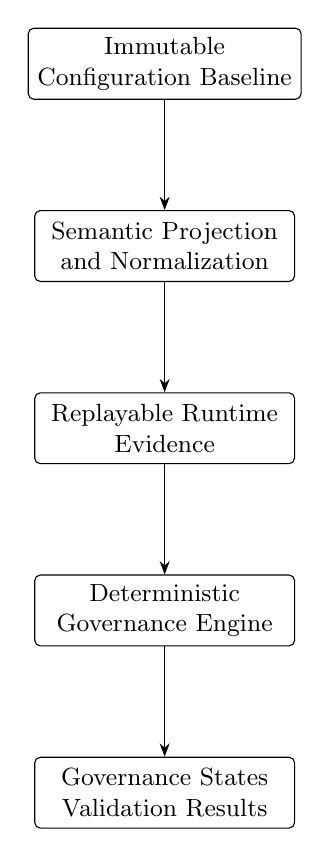
\begin{tikzpicture}[
    node distance=1.4cm,
    >=Stealth,
    box/.style={
        draw,
        rounded corners=2pt,
        align=center,
        minimum width=3.3cm,
        minimum height=0.9cm,
        font=\small
    }
]

\node[box] (baseline) {Immutable\\Configuration Baseline};

\node[box, below=of baseline] (projection) {Semantic Projection\\and Normalization};

\node[box, below=of projection] (runtime) {Replayable Runtime\\Evidence};

\node[box, below=of runtime] (engine) {Deterministic\\Governance Engine};

\node[box, below=of engine] (results) {Governance States\\Validation Results};

\draw[->] (baseline) -- (projection);
\draw[->] (projection) -- (runtime);
\draw[->] (runtime) -- (engine);
\draw[->] (engine) -- (results);

\end{tikzpicture}
    \caption{Deterministic governance pipeline supporting reproducibility and replicability. Immutable configuration baselines, semantic projection, replayable runtime evidence, and deterministic governance computation together enable independent reproduction of governance results without requiring deterministic LLM outputs.}
    \label{fig:reproducibility_pipeline}
\end{figure}

\subsection{Mitigation Strategies}
\label{sec:mitigation_strategies}

Although the preceding subsections identify several limitations affecting the present study, a number of methodological choices were deliberately adopted to reduce their impact on the reported results. Rather than attempting to maximize the breadth of the evaluation, the experimental methodology emphasizes internal consistency, deterministic governance semantics, and explicit separation between conceptual modeling, operationalization, and experimental validation.

First, the reference model was intentionally designed independently of any particular execution framework. The semantic projection architecture isolates framework-specific extraction mechanisms from the governance kernel, allowing the latter to remain unchanged across heterogeneous orchestration paradigms. This separation reduces implementation bias and facilitates the extension of the evaluation to additional frameworks without modifying the underlying governance semantics.

Second, the evaluation relies on normative governance scenarios rather than application-specific benchmarks. Each scenario targets a well-defined property of the reference model, such as lifecycle management, dependency propagation, assurance computation, baseline validation, or runtime governance. This scenario-driven methodology improves the traceability between the formal specification, the reference implementation, and the experimental evidence.

Third, reproducibility is reinforced through deterministic governance computation, immutable configuration revisions, canonical serialization, replayable runtime evidence, and automated validation procedures. These mechanisms ensure that governance outcomes depend exclusively on governed configurations and observed runtime events rather than on the stochastic behavior of the underlying language models.

In conclusion, this article deliberately distinguishes between the conceptual reference model, its formal governance semantics, the reference implementation, and the experimental evaluation. This separation avoids conflating theoretical contributions with implementation artifacts and allows future implementations to validate the same governance semantics independently of the current prototype.

Table~\ref{tab:mitigation_strategies} summarizes the principal threats identified in this section together with the corresponding mitigation strategies adopted throughout the study.

\begin{table}[t]
\caption{Summary of Threats and Mitigation Strategies}
\label{tab:mitigation_strategies}
\centering
\begin{tabular}{p{4.2cm}p{3.9cm}}
\toprule
\textbf{Threat} & \textbf{Mitigation Strategy} \\
\midrule
Limited framework coverage &
Evaluation across heterogeneous orchestration paradigms; framework-independent governance kernel. \\

Incomplete formal verification &
Executable formal semantics supported by deterministic implementation and normative validation scenarios. \\

Limited empirical generalization &
Conservative interpretation of results; explicit delimitation of the evaluation scope. \\

Implementation-dependent bias &
Separation between semantic projection, governance kernel, and framework adapters. \\

Experimental reproducibility &
Immutable revisions, replayable runtime events, canonical serialization, and automated validation suite. \\

Framework evolution &
Projection architecture designed to accommodate additional adapters without modifying the reference model. \\
\bottomrule
\end{tabular}
\end{table}

\subsection{Section Summary}
\label{sec:threats_summary}

The objective of this section has been to delimit the scope within which the conclusions of the present study should be interpreted. The identified threats do not challenge the internal consistency of the ACM reference model nor the coherence of its governance semantics. Instead, they primarily concern the breadth of the experimental validation, the current level of formal verification, and the extent to which the reported results can be generalized across the rapidly evolving landscape of agentic systems.

The experimental methodology intentionally favors methodological rigor over exhaustive coverage by combining a framework-independent governance representation, executable governance semantics, deterministic validation procedures, and reproducible experimental artifacts. Within this scope, the reported results provide credible evidence supporting the feasibility and expressiveness of the proposed governance model while avoiding claims that extend beyond the evaluated configurations.

These limitations naturally define the next stage of the research agenda. In particular, extending the empirical validation to additional orchestration paradigms, strengthening the formal verification of the governance semantics, and broadening the ecosystem supported by semantic projection represent logical continuations of the present work. These directions are discussed in the following section.

\section{Future Work}
\label{sec:future_work}

The ACM reference model introduced in this paper constitutes an initial step toward a framework-independent approach to the governance of agentic systems. The proposed metamodel, governance semantics, reference implementation, and experimental evaluation collectively demonstrate the feasibility of this approach within the scope considered in the present study. At the same time, the limitations identified in the previous section highlight several opportunities for extending both the theoretical foundations and the practical applicability of ACM.

Future research therefore naturally follows three complementary directions. The first concerns the evolution of the reference model itself to accommodate emerging abstractions while preserving its governance principles. The second focuses on strengthening the empirical and theoretical validation of the proposed semantics through broader experimental studies and formal verification. The long-term perspective is to position ACM as a common governance layer capable of interoperating with the rapidly expanding ecosystem of agentic development, deployment, and observability platforms.

\subsection{Extension of the Reference Model}
\label{sec:future_reference_model}

The reference model presented in this paper intentionally focuses on the minimal set of governance concepts required to represent heterogeneous agentic systems independently of their execution framework. This design choice favors conceptual stability and limits the number of core abstractions to those introducing distinct governance semantics. Nevertheless, the rapid evolution of agentic ecosystems will inevitably lead to the emergence of new configuration artifacts, interaction patterns, and execution abstractions that may require additional modeling capabilities.

A primary direction for future research is therefore the controlled evolution of the ACM metamodel while preserving its foundational design principles. Rather than continuously introducing framework-specific concepts into the core model, future extensions should remain guided by semantic necessity: a new abstraction should only become part of the reference model if it introduces governance properties that cannot be represented through the existing concepts and relationships. This principle preserves the framework independence of ACM while avoiding unnecessary growth of the metamodel.

An important example concerns reusable composite capabilities that are increasingly appearing under different names across modern agentic platforms, such as skills, reusable workflows, capability modules, or packaged execution components. Although these constructs differ in their implementation details, they frequently encapsulate existing governed artifacts—including prompts, tools, models, policies, workflows, and external resources—rather than introducing fundamentally new governance semantics. Consequently, many of these emerging abstractions can already be represented through semantic projection as governed composite configuration items without requiring modifications to the ACM core.

An additional extension concerns Retrieval-Augmented Generation (RAG) systems, which are becoming a fundamental building block of modern agentic applications. Rather than introducing a dedicated governance abstraction, ACM can represent RAG pipelines through the composition of existing configuration items, including embedding models, retrieval policies, vector indexes, knowledge repositories, prompt definitions, and retrieval components. This representation enables immutable versioning of the complete retrieval configuration, explicit provenance of derived vector indexes, and governance of retrieval policies independently of the underlying storage technology. Consequently, ACM can govern the evolution of retrieval-augmented systems without embedding retrieval-specific concepts into its core metamodel.

Another important direction concerns self-learning or continuously adaptive agents. Such systems challenge traditional configuration management because parts of their operational behavior may evolve autonomously through accumulated experience, parameter adaptation, or long-term memory updates. Extending ACM to distinguish immutable governed configurations from controlled runtime knowledge evolution would enable adaptive systems to remain auditable while preserving reproducibility of approved configurations. Future work should therefore investigate governance semantics capable of representing learning artifacts, adaptation boundaries, and evidence associated with autonomous configuration evolution.

Finally, the increasing adoption of interoperability protocols and workflow orchestration platforms, including Model Context Protocol (MCP), Agent-to-Agent (A2A) communication, and low-code orchestration environments such as n8n, provides another opportunity for extending the reference model. Rather than incorporating protocol-specific abstractions, ACM can represent these ecosystems through semantic projection of communication endpoints, external services, orchestration workflows, and interaction contracts into governed configuration items. This approach preserves the framework-independent nature of the reference model while enabling configuration governance across heterogeneous execution environments and emerging interoperability standards.

Future extensions may also address governance capabilities that extend beyond the scope of the current reference model. Examples include distributed governance across multiple organizations, federated configuration repositories, cross-system dependency management, richer policy composition mechanisms, and governance of long-lived autonomous ecosystems whose configuration evolves continuously over time. These extensions would broaden the applicability of ACM while preserving the separation between configuration governance and execution that constitutes one of its central architectural principles.

Ultimately, the long-term evolution of ACM should prioritize conceptual stability over feature accumulation. As with mature reference models in software engineering, the objective is not to mirror every innovation introduced by individual frameworks, but rather to identify the stable governance abstractions that remain applicable despite the continuous evolution of execution technologies. This philosophy enables the reference model to evolve incrementally while maintaining interoperability, explainability, and long-term sustainability.

\subsection{Broader Framework Validation}
\label{sec:future_framework_validation}

The empirical evaluation presented in this paper intentionally focuses on two representative orchestration paradigms in order to demonstrate the feasibility of framework-independent configuration governance. Although the successful semantic projection of LangGraph and CrewAI provides encouraging evidence supporting the proposed reference model, broader validation across the rapidly evolving landscape of agentic systems remains an essential research direction.

Future work should therefore extend the experimental corpus to additional execution frameworks exhibiting different orchestration principles and configuration abstractions. In particular, frameworks supporting dynamic handoffs, hierarchical delegation, event-driven coordination, decentralized multi-agent collaboration, or long-running autonomous workflows would provide valuable opportunities to evaluate the expressiveness of the ACM metamodel under substantially different execution models.

Beyond execution frameworks themselves, validation could also incorporate complementary components of the emerging AgentOps and LLMOps ecosystem. Provenance platforms, observability infrastructures, evaluation frameworks, and deployment management systems increasingly expose governance-relevant metadata that could naturally participate in semantic projection. Studying the integration of ACM with such platforms would provide additional evidence regarding the ability of the reference model to serve as a common governance layer across heterogeneous operational environments.

Another important direction concerns empirical validation at industrial scale. The current experiments intentionally emphasize semantic correctness rather than operational scalability. Future studies should therefore evaluate ACM on large agentic systems involving hundreds or thousands of governed configuration items, long-lived execution histories, continuously evolving baselines, and collaborative governance processes distributed across multiple development teams. Such evaluations would provide quantitative evidence regarding scalability, governance overhead, and operational usability in realistic production environments.

Ultimately, extending the experimental validation is not intended merely to increase the number of supported frameworks. Rather, it aims to progressively strengthen the empirical evidence supporting the central hypothesis of this work: that governance semantics can remain stable despite the continuous evolution of agentic execution technologies.

\subsection{Formal Verification of Governance Semantics}
\label{sec:future_formal_verification}

The governance semantics introduced in this paper are defined through a formal operational specification and validated through deterministic execution of the reference implementation. While this approach demonstrates the practical executability of the proposed semantics, it does not constitute a formal mathematical proof of their correctness. Establishing such guarantees represents an important direction for future research.

One immediate objective concerns the verification of the fixed-point propagation algorithm underlying governance state computation. Formal proofs could establish properties such as termination, determinism, convergence toward a unique governance state, and independence from evaluation order. Demonstrating these properties would strengthen confidence that governance decisions remain stable regardless of implementation details or execution strategies.

A second research direction involves the formal analysis of the lifecycle semantics themselves. The lifecycle state machines, dependency propagation rules, assurance composition mechanisms, and runtime governance semantics could be expressed within a formal verification framework in order to prove invariants such as transition consistency, absence of contradictory governance states, preservation of dependency constraints, and correctness of state propagation under arbitrary configuration topologies.

Beyond individual algorithms, future work may investigate the formal specification of the ACM reference model as a complete governance system. Model-checking techniques, temporal logic, theorem proving, or specification languages dedicated to distributed systems could be employed to verify global properties of the governance semantics and to detect inconsistencies automatically during the evolution of the reference model. Such approaches would complement the current implementation-based validation with machine-verifiable correctness guarantees.

Formal verification would facilitate the development of independent ACM implementations. By providing mathematically specified governance semantics rather than relying solely on behavioral equivalence with the reference implementation, future implementations could demonstrate conformance through proof of semantic equivalence instead of implementation similarity. This evolution would represent an important step toward establishing ACM as a stable and implementation-independent governance specification.

\subsection{Toward an Agentic Configuration Ecosystem}
\label{sec:future_ecosystem}

The rapid maturation of agentic software engineering has led to the emergence of a rich ecosystem of complementary technologies dedicated to development, deployment, observability, evaluation, provenance, and operational governance. Rather than replacing these existing tools, ACM is intended to provide a framework-independent governance layer capable of connecting heterogeneous components through a common semantic representation of governed configuration artifacts.

A promising direction for future research therefore consists in studying the integration of ACM with broader AgentOps and LLMOps ecosystems. Modern observability platforms increasingly collect execution traces, evaluation results, model usage metrics, cost information, and provenance metadata that constitute valuable inputs for governance processes. Conversely, governance decisions produced by ACM could enrich these platforms with lifecycle status, assurance levels, configuration lineage, dependency analysis, and compliance information, providing a higher semantic level for operational monitoring.

Another important perspective concerns the integration of ACM with software engineering infrastructures. Continuous integration and deployment pipelines, software configuration management systems, artifact repositories, and supply-chain security mechanisms already manage the lifecycle of conventional software assets. Extending these infrastructures to incorporate governed agentic configuration items would enable unified governance across both traditional software components and AI-native artifacts while preserving traceability throughout the complete development lifecycle.

Beyond tooling integration, future work may explore the definition of interoperable governance services exposing standardized interfaces for semantic projection, configuration validation, governance state computation, and provenance exchange. Such services would facilitate the development of heterogeneous toolchains in which execution frameworks, observability platforms, deployment systems, and governance engines cooperate while remaining independently evolvable.

Ultimately, the long-term objective is to establish ACM not as another execution platform, but as a common semantic governance layer capable of interconnecting the diverse technologies that increasingly compose modern agentic software ecosystems.

\subsection{Standardization Perspectives}
\label{sec:future_standardization}

The absence of a common vocabulary and shared governance abstractions currently represents one of the principal obstacles to interoperability across agentic systems. While execution frameworks continue to evolve rapidly, equivalent concepts are frequently described using framework-specific terminology, making configuration exchange, governance portability, and comparative evaluation unnecessarily difficult.

The ACM reference model represents an initial step toward addressing this fragmentation by proposing a framework-independent conceptual vocabulary together with formally defined governance semantics. Although the present work does not aim to establish a standard, it provides a structured foundation upon which future community discussions regarding interoperable governance models may build.

Future research may therefore investigate the definition of standardized exchange formats for governed configuration items, semantic projection interfaces, governance evidence, provenance information, and lifecycle metadata. Such specifications would facilitate interoperability between heterogeneous execution frameworks while allowing governance information to remain portable independently of implementation technologies. Likewise, standardized conformance criteria could enable independent implementations to demonstrate semantic compatibility with the ACM reference model while preserving implementation freedom.

The maturation of ACM may also benefit from collaboration with broader software engineering and artificial intelligence communities working on software configuration management, software supply-chain security, provenance, and AI governance. Aligning ACM with existing standards whenever appropriate would facilitate its integration into established engineering practices while reducing duplication of concepts that are already well understood in adjacent disciplines.

Ultimately, the long-term ambition is not to standardize a particular implementation, but to encourage convergence toward a shared governance language for agentic systems towards an agentic configuration ecosystem. By separating governance semantics from execution technologies, ACM provides a stable conceptual foundation that could evolve collaboratively as the agentic landscape continues to mature. Such convergence would improve interoperability, reproducibility, auditability, and long-term sustainability across heterogeneous agentic platforms. Such anglobal agentic ecosystem, including ACM, could progressively evolve toward interoperable configuration exchange and, ultimately, contribute to future standardization efforts for governed agentic systems.

\section{Conclusion}
\label{sec:conclusion}

The rapid evolution of agentic software engineering has fundamentally transformed the role of configuration artifacts. Prompts, tools, execution graphs, policies, models, runtime state, and provenance have become first-class engineering assets whose governance can no longer rely solely on traditional software configuration management practices. At the same time, the increasing diversity of orchestration frameworks has introduced heterogeneous configuration abstractions, making governance difficult to reproduce, audit, and compare across platforms.

This paper introduced Agentic Configuration Management (ACM), a framework-independent governance representation for the governance of agentic systems. Rather than proposing another execution framework, ACM separates governance semantics from execution technologies through a unified representation of governed configuration items, immutable revisions, semantic relationships, deterministic lifecycle management, assurance semantics, and runtime governance. This separation enables heterogeneous agentic systems to be represented within a common governance model while preserving the flexibility of existing orchestration frameworks.

Beyond the conceptual contribution, the paper demonstrated that the proposed semantics can be operationalized through a reference implementation and evaluated using representative orchestration paradigms. The experimental results show that heterogeneous agentic configurations can be semantically projected into a common governance representation while preserving the information required for deterministic governance decisions. Although the current evaluation remains intentionally limited in scope, it provides initial empirical evidence supporting the feasibility of framework-independent configuration governance for agentic systems.

More broadly, this work argues that governance should become an explicit architectural layer of agentic software engineering rather than an implementation-specific concern embedded within individual execution frameworks. By introducing a common vocabulary, formally defined governance semantics, and a framework-independent governance representation, ACM establishes a foundation upon which future research can investigate interoperability, formal verification, scalable governance, and standardized configuration management practices for increasingly autonomous AI systems.

Ultimately, the contribution of ACM is not to prescribe how agentic systems should execute, but to provide a stable semantic foundation for governing how they are specified, versioned, validated, traced, and evolved. As agentic ecosystems continue to diversify, such a separation between execution and governance may become an essential prerequisite for building reproducible, auditable, interoperable, and trustworthy AI systems.

%%%%%%%%%%%%%%%%%%%%%%%%%%%%%%%%%%%%%%%%%%%%%%%%%%%%%%%%%%%%%%%%%%%%%%%%%%%%%%%%
\appendices
\section{Appendix}
\label{appendix}
\subsection{Related Work}
\label{appendix:related_work}
\subsubsection{Framework Comparison}
Table~\ref{tab:framework_comparison} summarizes representative characteristics of several widely used agentic frameworks.
\begin{table*}[t]
	\centering
	\caption{Representative characteristics of widely used agentic frameworks. The comparison illustrates the diversity of execution paradigms while highlighting the absence of a common configuration representation.}
	\label{tab:framework_comparison}
	
	\renewcommand{\arraystretch}{1.15}
	
	\begin{tabular}{p{3.2cm}p{3.1cm}p{3.4cm}p{3.4cm}c}
		\toprule
		\textbf{Framework}
		&
		\textbf{Primary Paradigm}
		&
		\textbf{Execution Model}
		&
		\textbf{Native Configuration Abstraction}
		\\
		\midrule
		
		LangGraph
		&
		State graph
		&
		Explicit graph execution
		&
		Nodes, edges and shared state
		\\
		
		CrewAI
		&
		Role-based multi-agent
		&
		Agents, tasks and crews
		&
		Agents, tasks, crews and flows
		\\
		
		OpenAI Agents SDK
		&
		Delegation-based agents
		&
		Handoffs and tool orchestration
		&
		Agents, tools and handoffs
		\\
		
		Microsoft Agent Framework
		&
		Workflow orchestration
		&
		Agent workflows
		&
		Workflow definitions
		\\
		
		Google ADK
		&
		Hierarchical agents
		&
		Multi-agent orchestration
		&
		Agent hierarchies
		\\
		
		\bottomrule
	\end{tabular}
	
\end{table*}
\subsubsection{Gap Analysis}
The Table ~\ref{tab:gap_analysis_detailed} supports a comparative gap analysis between the different governance aproaches.
\begin{table*}[t]
	\centering
	\caption{Detailed rationale supporting the comparative gap analysis
		presented in Table~\ref{tab:gap_analysis}.}
	\label{tab:gap_analysis_detailed}
	
	\footnotesize
	\setlength{\tabcolsep}{3pt}
	\renewcommand{\arraystretch}{1.18}
	
	\begin{tabularx}{\textwidth}{
			>{\RaggedRight\arraybackslash}p{3.25cm}
			C{1.05cm}
			C{1.15cm}
			C{1.45cm}
			C{1.30cm}
			C{0.85cm}
			Y
		}
		\toprule
		
		\textbf{Governance capability}
		&
		\makecell{\textbf{SCM}}
		&
		\makecell{\textbf{AI}\\\textbf{Gov.}}
		&
		\makecell{\textbf{LLMOps /}\\\textbf{AgentOps}}
		&
		\makecell{\textbf{Agent}\\\textbf{frameworks}}
		&
		\makecell{\textbf{ACM}}
		&
		\textbf{Rationale}
		\\
		
		\midrule
		
		Configuration identification
		&
		$\checkmark$
		&
		$\sim$
		&
		$\sim$
		&
		$\sim$
		&
		$\checkmark$
		&
		SCM explicitly identifies configuration items.
		Other approaches identify only the artefacts relevant to their
		respective governance, operational, or execution objectives.
		ACM represents heterogeneous artefacts as governed ACI revisions.
		\\
		
		Version management
		&
		$\checkmark$
		&
		--
		&
		$\sim$
		&
		$\sim$
		&
		$\checkmark$
		&
		SCM provides mature version control.
		LLMOps platforms and agent frameworks version selected artefacts,
		such as prompts or workflows, but not complete governed
		configurations.
		ACM assigns immutable revisions to every governed artefact.
		\\
		
		Configuration provenance
		&
		$\sim$
		&
		$\checkmark$
		&
		$\checkmark$
		&
		$\sim$
		&
		$\checkmark$
		&
		SCM preserves software history, while AI governance and LLMOps
		emphasize provenance, accountability, and traceability.
		Frameworks expose partial execution provenance.
		ACM links configuration, revision, runtime, and evidence provenance.
		\\
		
		Dependency traceability
		&
		$\checkmark$
		&
		$\sim$
		&
		$\checkmark$
		&
		$\sim$
		&
		$\checkmark$
		&
		SCM manages software dependencies, and LLMOps relates selected
		artefacts such as prompts, traces, and evaluations.
		Frameworks expose dependencies through native abstractions.
		ACM explicitly models typed dependencies across heterogeneous
		configuration artefacts.
		\\
		
		Execution observability
		&
		--
		&
		$\sim$
		&
		$\checkmark$
		&
		$\checkmark$
		&
		$\checkmark$
		&
		Execution monitoring is not a primary SCM capability.
		AI governance recommends monitoring, whereas LLMOps platforms and
		agent frameworks provide traces and runtime telemetry.
		ACM incorporates normalized runtime observations into its governance
		representation.
		\\
		
		Lifecycle governance
		&
		$\sim$
		&
		$\checkmark$
		&
		$\sim$
		&
		$\sim$
		&
		$\checkmark$
		&
		SCM governs controlled software evolution, and AI governance defines
		processes across the AI lifecycle.
		Operational platforms and frameworks mainly address deployment or
		execution stages.
		ACM governs the lifecycle of exact configuration revisions.
		\\
		
		Framework-independent representation
		&
		--
		&
		--
		&
		--
		&
		--
		&
		$\checkmark$
		&
		Existing approaches remain centred on software artefacts,
		organizational processes, operational platforms, or native execution
		models.
		ACM provides a framework-independent representation of governed
		agentic configurations.
		\\
		
		Unified configuration model
		&
		--
		&
		--
		&
		--
		&
		--
		&
		$\checkmark$
		&
		No other family combines heterogeneous artefacts, immutable
		revisions, typed dependencies, governance semantics, and runtime
		traceability within one reference model.
		This integration constitutes ACM's primary contribution.
		\\
		
		\bottomrule
	\end{tabularx}
	
	\vspace{0.4em}
	
	{\scriptsize
		$\checkmark$ Fully addressed
		\hspace{1em}
		$\sim$ Partially addressed
		\hspace{1em}
		-- Not provided as a primary capability.
	}
	
\end{table*}
	

\subsection{Governance Semantics}
%%%%%%%%%%%%%%%%%%%%%%%%%%%%%%%%%%%%%%%%%%%%%%%%%%%%%%%%%%%%%%%%%%%%%%%%%%%%%%%%
\subsubsection{Orthogonality of Governance State Machines}
\label{appendix:governance_orthogonality}
The four governance state machines satisfy an orthogonality property.

\paragraph{Definition 1 (Orthogonality).}

Two governance dimensions

\[
X
\]

and

\[
Y
\]

are orthogonal if transitions performed within

\[
X
\]

do not directly modify the internal state of

\[
Y.
\]

Instead, interactions occur only through explicit evaluation functions or
propagation algorithms.

Formally,

\begin{equation}
\delta_X
\neq
\delta_Y
\label{eq:app_orth1}
\end{equation}

and

\begin{equation}
\forall
\sigma
\in
\Sigma_X,
\quad
\delta_Y(s,\sigma)
=
s,
\label{eq:app_orth2}
\end{equation}

unless a propagation rule explicitly connects the two dimensions.

This design eliminates hidden side effects and enables deterministic reasoning
over governance decisions.

%%%%%%%%%%%%%%%%%%%%%%%%%%%%%%%%%%%%%%%%%%%%%%%%%%%%%%%%%%%%%%%%%%%%%%%%%%%%%%%%
\subsubsection{Impact Propagation Formalism}
\label{appendix:impact_propagation}
\paragraph{Dependency Graph}

Let

\[
G=(V,E)
\]

denote the directed governance graph defined previously.

Each edge

\[
(u,v)\in E
\]

represents a governance dependency from revision

\[
u
\]

towards revision

\[
v.
\]

An edge indicates that the governance state of

\[
v
\]

depends, directly or indirectly, on properties associated with

\[
u.
\]

Dependencies are independent of implementation details and therefore apply
uniformly to prompts, agents, workflows, tools, datasets, execution plans,
runtime artifacts and governance policies.

%%%%%%%%%%%%%%%%%%%%%%%%%%%%%%%%%%%%%%%%%%%%%%%%%%%%%%%%%%%%%%%%%%%%%%%%%%%%%%%%
\paragraph{Local Impact}

A governance event affecting one revision first generates a local impact.

Let

\[
\Delta(v)
\]

denote a modification applied to revision

\[
v.
\]

Typical governance events include

\begin{itemize}
	\item prompt modification,
	\item parameter update,
	\item dependency replacement,
	\item policy modification,
	\item tool substitution,
	\item workflow restructuring,
	\item runtime extension.
	\item etc.
\end{itemize}

Immediately after the modification,

\[
I(v)=Local.
\]

The modified revision therefore becomes the origin of an impact propagation
process.

%%%%%%%%%%%%%%%%%%%%%%%%%%%%%%%%%%%%%%%%%%%%%%%%%%%%%%%%%%%%%%%%%%%%%%%%%%%%%%%%
\paragraph{Propagation Operator}

Impact propagates along outgoing governance dependencies.

Let

\begin{equation}
Succ(v)
=
\{
u
\mid
(v,u)\in E
\}
\label{eq:app_prop_op1}
\end{equation}

denote the successor set of

\[
v.
\]

The propagation operator

\begin{equation}
P
:
2^V
\rightarrow
2^V
\label{eq:app_prop_op2}
\end{equation}

is recursively defined as

\begin{equation}
P(X)
=
X
\cup
\bigcup_{v\in X}
Succ(v).
\label{eq:app_prop_op3}
\end{equation}

The complete impact closure corresponds to the least fixed point

\begin{equation}
P^\ast(X)
=
\lim_{k\rightarrow\infty}
P^{k}(X).
\label{eq:app_prop_op3}
\end{equation}

Every node belonging to

\begin{equation}
P^\ast(\{v\})
\label{eq:app_prop_op4}
\end{equation}

is considered impacted by the initial modification.

Consequently,

\begin{equation}
I(u)=Propagated,
\qquad
\forall
u
\in
P^\ast(\{v\})
\setminus
\{v\}.
\label{eq:app_prop_op5}
\end{equation}

%%%%%%%%%%%%%%%%%%%%%%%%%%%%%%%%%%%%%%%%%%%%%%%%%%%%%%%%%%%%%%%%%%%%%%%%%%%%%%%%
\subsubsection{Eligibility Semantics Formalism}
\label{appendix:eligibility_semantics}
\paragraph{Normative Evaluation Rules}
\label{appendix:eligibility_rules}

The reference model intentionally does not prescribe a unique implementation
algorithm.

Instead, it specifies normative decision constraints.

An implementation shall satisfy the following rules.

\paragraph{Rule E1.}

If

\[
Q(v)=Invalid,
\]

then

\[
E(v)=Blocked.
\]

%%%%%%%%%%%%%%%%%%%%%%%%%%%%%%%%%%%%%%%%%%%%%%%%%%

\paragraph{Rule E2.}

If

\[
A(v)=Unassessed,
\]

execution cannot be considered fully eligible.

%%%%%%%%%%%%%%%%%%%%%%%%%%%%%%%%%%%%%%%%%%%%%%%%%%

\paragraph{Rule E3.}

If propagated impact remains unresolved,

\[
I(v)=Propagated,
\]

eligibility shall be recomputed before execution.

%%%%%%%%%%%%%%%%%%%%%%%%%%%%%%%%%%%%%%%%%%%%%%%%%%

\paragraph{Rule E4.}

Lifecycle states

Deprecated

and

Archived

shall never produce

Eligible.

%%%%%%%%%%%%%%%%%%%%%%%%%%%%%%%%%%%%%%%%%%%%%%%%%%

\paragraph{Rule E5.}

Only governance-compliant revisions may reach the

Eligible

state.

%%%%%%%%%%%%%%%%%%%%%%%%%%%%%%%%%%%%%%%%%%%%%%%%%%%%%%%%%%%%%%%%%%%%%%%%%%%%%%%%
\paragraph{Eligibility Ordering}

Eligibility states satisfy the total order

\begin{equation}
Blocked
<
Restricted
<
Eligible.
\label{eq:app_elig1}
\end{equation}

This ordering allows governance policies to define conservative aggregation
operators.

For example,

\begin{equation}
min(E_1,E_2,\ldots,E_n)
\label{eq:app_elig2}
\end{equation}

naturally computes the eligibility of composite configurations.

%%%%%%%%%%%%%%%%%%%%%%%%%%%%%%%%%%%%%%%%%%%%%%%%%%%%%%%%%%%%%%%%%%%%%%%%%%%
\paragraph{Eligibility Composition}

Let

\begin{equation}
C
=
\{
v_1,
...
,
v_n
\}
\label{eq:app_elig3}
\end{equation}

denote a composite workflow.

Its global eligibility is defined as

\begin{equation}
E(C)
=
\min
\{
E(v_i)
\}.
\label{eq:app_elig4}
\end{equation}

Consequently, a workflow cannot be considered fully deployable if one of its
mandatory governance components remains blocked.

Alternative aggregation operators may be introduced for optional dependencies
without modifying the underlying semantic model.

%%%%%%%%%%%%%%%%%%%%%%%%%%%%%%%%%%%%%%%%%%%%%%%%%%%%%%%%%%%%%%%%%%%%%%%%%%%%%%%%
\subsubsection{Determinism}

Eligibility evaluation satisfies three properties.

\paragraph{Property E1.}

Determinism.

The same governance descriptor always produces the same eligibility state.

\paragraph{Property E2.}

Composability.

Eligibility evaluation scales recursively from individual revisions to complete
configuration graphs.

\paragraph{Property E3.}

Extensibility.

Additional governance dimensions may be incorporated into

\[
f
\]

without modifying the semantics of existing dimensions.

\subsection{Assurance Semantics Formalism}
\label{appendix:assurance_semantics}
%%%%%%%%%%%%%%%%%%%%%%%%%%%%%%%%%%%%%%%%%%%%%%%%%%%%%%%%%%%%%%%%%%%%%%%%%%%%%%%%
\subsubsection{Evidence Coverage}
\label{appendix:evidence_coverage}
Assurance is computed from the coverage of governance evidence.

Let

\begin{itemize}
	\item \(R(v)\) denote the set of evidence categories required for revision
	\(v\);
	\item \(E(v)\subseteq R(v)\) denote the subset of required evidence that is
	currently applicable and valid.
\end{itemize}

The evidence coverage ratio is defined as

\begin{equation}
	Cover(v)
	=
	\begin{cases}
		1,
		&
		|R(v)|=0,
		\\[0.3em]
		\dfrac{|E(v)|}{|R(v)|},
		&
		\text{otherwise.}
	\end{cases}
	\label{eq:coverage_assurance}
\end{equation}

Equation~(\ref{eq:coverage_assurance}) measures only the completeness of available
evidence. It deliberately ignores whether the associated evaluations succeeded
or failed.

The assurance state is then derived from this coverage according to

\begin{equation}
	A_n(v)
	=
	\begin{cases}
		\texttt{unassessed},
		&
		Cover(v)=0,
		\\[0.3em]
		\texttt{partially\_assessed},
		&
		0<Cover(v)<1,
		\\[0.3em]
		\texttt{assessed},
		&
		Cover(v)=1.
	\end{cases}
	\label{eq:assurance_from_coverage}
\end{equation}

Unlike probabilistic confidence measures frequently encountered in machine
learning, ACM assurance is therefore deterministic and entirely reproducible.
Only evidence satisfying Equation~(\ref{eq:applicable_evidence}) contributes to the
coverage defined in Equation~(\ref{eq:coverage_assurance}).

%%%%%%%%%%%%%%%%%%%%%%%%%%%%%%%%%%%%%%%%%%%%%%%%%%%%%%%%%%%%%%%%%%%%%%%%%%%%%%%%
\subsubsection{Composite Assurance}

Composite governance artifacts cannot inherit assurance directly from their
components.

Instead, ACM evaluates the assurance of a composite from:

\begin{enumerate}
	\item its own evidence;
	\item the effective assurance of the required dependencies participating in
	the composition.
\end{enumerate}

Let

\[
Req(v)
\]

denote the set of required dependencies participating in the assurance
evaluation of revision \(v\).

The effective assurance of a composite is therefore defined as

\begin{equation}
	A_n^{eff}(v)
	=
	\begin{cases}
		\texttt{unassessed},
		&
		A_n(v)=\texttt{unassessed},
		\\[0.4em]
		\texttt{partially\_assessed},
		&
		A_n(v)\neq\texttt{assessed}
		\;\vee\;
		\exists u\in Req(v),
		A_n^{eff}(u)\neq\texttt{assessed},
		\\[0.4em]
		\texttt{assessed},
		&
		A_n(v)=\texttt{assessed}
		\;\land\;
		\forall u\in Req(v),
		A_n^{eff}(u)=\texttt{assessed}.
	\end{cases}
	\label{eq:effective_assurance}
\end{equation}

Equation~(\ref{eq:effective_assurance}) expresses a conservative propagation
policy: incomplete assurance of any mandatory dependency prevents the composite
from reaching the highest assurance level.

%%%%%%%%%%%%%%%%%%%%%%%%%%%%%%%%%%%%%%%%%%%%%%%%%%%%%%%%%%%%%%%%%%%%%%%%%%%%%%%%
\subsubsection{Assurance Invariants}

The assurance semantics satisfy the following invariants.

\paragraph{Invariant A1 (Revision Specificity).}

Every assurance assessment is attached to one immutable revision only.

\begin{equation}
	Evidence(e)
	\Longrightarrow
	revision(e)
	=
	revision(v).
	\label{eq:assurance_inv1}
\end{equation}

\paragraph{Invariant A2 (Evidence Completeness).}

A revision cannot reach the state
\texttt{assessed}
unless every required evidence category is covered.

\begin{equation}
	A_n(v)=\texttt{assessed}
	\Longrightarrow
	Cover(v)=1.
	\label{eq:assurance_inv2}
\end{equation}

\paragraph{Invariant A3 (Propagation Consistency).}

The effective assurance of a composite cannot exceed the effective assurance of
its least assured mandatory dependency.

\begin{equation}
	A_n^{eff}(v)
	\preceq
	\min_{u\in Req(v)}
	A_n^{eff}(u),
	\label{eq:assurance_inv3}
\end{equation}

where the ordering relation is

\begin{equation}[
\texttt{unassessed}
\prec
\texttt{partially\_assessed}
\prec
\texttt{assessed}.
\label{eq:assurance_hierarchy}
\end{equation}

%%%%%%%%%%%%%%%%%%%%%%%%%%%%%%%%%%%%%%%%%%%%%%%%%%%%%%%%%%%%%%%%%%%%%%%%%%%%%%%%
\subsection{Governance State Propagation Formalism}
\label{appendix:state_propagation}
\subsubsection{Governance Propagation Principles}

Unlike traditional dependency propagation mechanisms, ACM distinguishes four
independent propagation mechanisms.

\paragraph{Lifecycle propagation.}

Lifecycle states never propagate directly.

A dependency becoming
\texttt{deprecated}
does not modify the lifecycle state of its parent.

\paragraph{Impact propagation.}

Impact propagates along every relationship marked as
\texttt{impact=true}.

The purpose of impact propagation is to identify which configuration items may
require reassessment.

\paragraph{Assurance propagation.}

Assurance propagates only through relationships declared as assurance
dependencies.

Its objective is to determine whether previously established evidence remains
sufficient for composite artifacts.

\paragraph{Eligibility propagation.}

Eligibility propagates according to the relationship policy and determines
whether governance operations such as validation or baseline release remain
authorized.

This separation avoids conflating fundamentally different governance concepts.

%%%%%%%%%%%%%%%%%%%%%%%%%%%%%%%%%%%%%%%%%%%%%%%%%%%%%%%%%%%%%%%%%%%%%%%%%%%%%%%%
\subsubsection{Impact Propagation}

Let

\[
I(v)
\]

denote the impact state of revision
$v$.

Whenever a governance event modifies a configuration item, the local impact is
propagated to all reachable dependent artifacts.

Let

\[
Succ(v)
\]

denote the successors of
$v$
within
$G_c$.

Impact propagation is defined recursively by

\begin{equation}
	I(u)
	=
	\max
	\left(
	I(u),
	I(v)
	\right),
	\qquad
	\forall
	u\in Succ(v)
	\label{eq:impact_propagation}
\end{equation}

using the ordering

\[
current
<
impacted
<
stale.
\]

The operator
$\max$
therefore propagates the most severe impact state.

This mechanism guarantees that every potentially affected configuration item is
explicitly identified before any governance decision is taken.

\begin{table}[ht]
	\caption{Impact state transition matrix.}
	\label{tab:impact_transition_matrix}
	\centering
	\small
	\begin{tabular}{llll}
		\toprule
		\textbf{From} & \textbf{To} & \textbf{Allowed} & \textbf{Typical Trigger} \\
		\midrule
		Not Impacted & Impacted & $\checkmark$ & Dependency change detected \\
		Impacted & Not Impacted & $\checkmark$ & Dependency re-evaluated and stabilized \\
		\bottomrule
	\end{tabular}
\end{table}

%%%%%%%%%%%%%%%%%%%%%%%%%%%%%%%%%%%%%%%%%%%%%%%%%%%%%%%%%%%%%%%%%%%%%%%%%%%%%%%%
\subsubsection{Quality Propagation}

Quality propagation differs fundamentally from impact propagation.

The intrinsic quality assigned to an ACI revision never changes as a
consequence of dependency evolution.

Instead, ACM computes an effective quality from the dependency graph.

Let

\[
Q_d(v)
\]

denote the declared quality,

and

\[
Q_e(v)
\]

the effective quality.

For the set of mandatory dependencies

\[
Req(v),
\]

the propagated quality is

\begin{equation}
	Q_e(v)
	=
	worst
	\left(
	Q_d(v),
	Q_e(u),
	u\in Req(v)
	\right)
	\label{eq:quality_propagation}
\end{equation}

according to the ordering

\[
ok
<
unknown
<
to\_improve
<
nok.
\]

Consequently, a mandatory dependency evaluated as
\texttt{nok}
prevents the composite artifact from reaching an effective quality better than
\texttt{nok},
while preserving the declared quality originally assigned to the revision.

\begin{table}[ht]
	\caption{Governance quality state transition matrix.}
	\label{tab:quality_transition_matrix}
	\centering
	\small
	\begin{tabular}{llll}
		\toprule
		\textbf{From} & \textbf{To} & \textbf{Allowed} & \textbf{Typical Trigger} \\
		\midrule
		Unknown & Evaluating & $\checkmark$ & Evaluation initiated \\
		Evaluating & Validated & $\checkmark$ & All validation criteria satisfied \\
		Evaluating & Warning & $\checkmark$ & Non-blocking issue detected \\
		Evaluating & Invalid & $\checkmark$ & Blocking issue detected \\
		Validated & Evaluating & $\checkmark$ & Re-evaluation required \\
		Warning & Evaluating & $\checkmark$ & Re-evaluation required \\
		Invalid & Evaluating & $\checkmark$ & Configuration modified or corrected \\
		\bottomrule
	\end{tabular}
\end{table}

%%%%%%%%%%%%%%%%%%%%%%%%%%%%%%%%%%%%%%%%%%%%%%%%%%%%%%%%%%%%%%%%%%%%%%%%%%%%%%%%
\subsubsection{Assurance Propagation}

Assurance propagation extends the effective assurance model introduced in the
previous subsection.

Only relationships explicitly marked as assurance dependencies contribute to
the propagated assurance.

Let

\[
Req_A(v)
\]

denote the subset of dependencies satisfying

\[
assurance=true.
\]

Effective assurance becomes

\begin{equation}
	A_n^{eff}(v)
	=
	combine
	\left(
	A_n(v),
	A_n^{eff}(u),
	u\in Req_A(v)
	\right)
	\label{eq:assurance_propagation}
\end{equation}

where the
\texttt{combine}
operator follows the conservative semantics defined in
Section~\ref{subsec:assurance_semantics}.

Unlike quality propagation, assurance additionally depends on the applicability
of the supporting evidence. A dependency becoming
\texttt{stale}
may therefore downgrade assurance without affecting quality.

\begin{table}[ht]
	\caption{Assurance state transition matrix.}
	\label{tab:assurance_transition_matrix}
	\centering
	\small
	\begin{tabular}{llll}
		\toprule
		\textbf{From} & \textbf{To} & \textbf{Allowed} & \textbf{Typical Trigger} \\
		\midrule
		Unassessed & Partially Assessed & $\checkmark$ & Partial evidence becomes available \\
		Unassessed & Assessed & $\checkmark$ & Required evidence complete \\
		Partially Assessed & Assessed & $\checkmark$ & Remaining evidence completed \\
		Assessed & Partially Assessed & $\checkmark$ & Part of the evidence becomes invalid \\
		Assessed & Unassessed & $\checkmark$ & Required evidence withdrawn or invalidated \\
		Partially Assessed & Unassessed & $\checkmark$ & Applicable evidence no longer available \\
		\bottomrule
	\end{tabular}
\end{table}

%%%%%%%%%%%%%%%%%%%%%%%%%%%%%%%%%%%%%%%%%%%%%%%%%%%%%%%%%%%%%%%%%%%%%%%%%%%%%%%%
\subsubsection{Eligibility Propagation}

Eligibility determines whether a governance operation remains authorized.

Eligibility depends simultaneously on

\begin{itemize}
	\item lifecycle,
	\item effective quality,
	\item effective assurance,
	\item propagated impact,
	\item relationship policies.
\end{itemize}

Let

\[
El(v)
\]

denote the eligibility state of revision
$v$.

The propagated eligibility is

\begin{equation}
	El(v)
	=
	f
	\left(
	L(v),
	Q_e(v),
	A_n^{eff}(v),
	I(v),
	\Pi(E_v)
	\right)
	\label{eq:eligibility_propagation}
\end{equation}

where

\[
f
\]

is the deterministic governance evaluation function introduced previously.

Eligibility therefore represents the synthesis of all governance dimensions
rather than an independent property.

\begin{table}[ht]
	\caption{Eligibility state transition matrix.}
	\label{tab:eligibility_transition_matrix}
	\centering
	\small
	\begin{tabular}{llll}
		\toprule
		\textbf{From} & \textbf{To} & \textbf{Allowed} & \textbf{Typical Trigger} \\
		\midrule
		Eligible & Warning & $\checkmark$ & Non-blocking governance issue detected \\
		Eligible & Blocked & $\checkmark$ & Mandatory governance constraint violated \\
		Warning & Eligible & $\checkmark$ & Advisory issue resolved \\
		Warning & Blocked & $\checkmark$ & Mandatory violation detected \\
		Blocked & Warning & $\checkmark$ & Partial remediation completed \\
		Blocked & Eligible & $\checkmark$ & All blocking conditions resolved \\
		\bottomrule
	\end{tabular}
\end{table}

%%%%%%%%%%%%%%%%%%%%%%%%%%%%%%%%%%%%%%%%%%%%%%%%%%%%%%%%%%%%%%%%%%%%%%%%%%%%%%%%
\subsubsection{Normative Invariants}

Governance propagation satisfies the following invariants.

\paragraph{Invariant GP1 (Lifecycle Independence).}

Lifecycle states never propagate.

\begin{equation}
	L(u)\neq L(v)
	\not\Rightarrow
	L(v)=L(u).
	\label{eq:gp1}
\end{equation}

\paragraph{Invariant GP2 (Conservative Assurance).}

Effective assurance cannot exceed the assurance of its least assured mandatory
dependency.

\begin{equation}
	A_n^{eff}(v)
	\preceq
	\min_{u\in Req_A(v)}
	A_n^{eff}(u).
	\label{eq:gp2}
\end{equation}

\paragraph{Invariant GP3 (Blocking Dependencies).}

A mandatory dependency evaluated as
\texttt{nok}
forces the effective quality of every dependent composite to
\texttt{nok}.

\begin{equation}
	Q_e(u)=nok
	\Longrightarrow
	Q_e(v)=nok,
	\quad
	u\in Req(v).
	\label{eq:gp3}
\end{equation}

\paragraph{Invariant GP4 (Deterministic Propagation).}

For identical configuration graphs, governance events and propagation policies,
the resulting governance state is unique.

\begin{equation}
	Propagate
	(G_c,\Sigma,\Pi)
	=
	Propagate
	(G_c,\Sigma,\Pi).
	\label{eq:gp4}
\end{equation}

%%%%%%%%%%%%%%%%%%%%%%%%%%%%%%%%%%%%%%%%%%%%%%%%%%%%%%%%%%%%%%%%%%%%%%%%%%%%%%%%
\subsection{Formal Properties of Governance Propagation}
\label{appendix:fixed_point_proofs}

This appendix provides the formal justification of the fixed-point semantics
introduced in Section~\ref{subsec:fixed_point_semantics}. The proofs rely only
on the assumptions explicitly stated by the ACM governance model, namely a
finite configuration graph, finite governance state spaces, and monotone
relationship transfer functions.

%%%%%%%%%%%%%%%%%%%%%%%%%%%%%%%%%%%%%%%%%%%%%%%%%%%%%%%%%%%%%%%%%%%%%%%%%%%%%%%

\subsection{Finite Lattice Structure}

The propagation domain is defined as the product lattice

\begin{equation}
\mathcal{L}
=
\mathcal{S}^{V_c},
\end{equation}

where

\begin{equation}
\mathcal{S}
=
\mathcal{I}
\times
\mathcal{Q}
\times
\mathcal{A}
\times
\mathcal{E}.
\end{equation}

Each component lattice is finite because every governance dimension is defined
over a finite ordered set.

Consequently,

\begin{equation}
|\mathcal{S}|
<
\infty.
\end{equation}

Since the configuration graph contains a finite number of revisions,

\begin{equation}
|V_c|
<
\infty,
\end{equation}

the product lattice

\begin{equation}
\mathcal{L}
=
\mathcal{S}^{V_c}
\end{equation}

is itself finite.

%%%%%%%%%%%%%%%%%%%%%%%%%%%%%%%%%%%%%%%%%%%%%%%%%%%%%%%%%%%%%%%%%%%%%%%%%%%%%%%

\subsection{Proof of Monotonicity}

The global propagation operator

\begin{equation}
F:\mathcal{L}\rightarrow\mathcal{L}
\end{equation}

is defined component-wise by

\begin{equation}
F(X)(v)
=
X(v)
\sqcup
B(v)
\sqcup
\bigvee_{u\in Pred(v)}
\tau_{(u,v)}
(X(u)).
\end{equation}

Assume

\begin{equation}
X
\sqsubseteq
Y.
\end{equation}

By definition of the product order,

\begin{equation}
X(u)
\sqsubseteq
Y(u)
\qquad
\forall u\in V_c.
\end{equation}

Since every relationship transfer function is monotone,

\begin{equation}
X(u)
\sqsubseteq
Y(u)
\Longrightarrow
\tau_{(u,v)}(X(u))
\sqsubseteq
\tau_{(u,v)}(Y(u)).
\end{equation}

The lattice join operator is monotone with respect to each of its operands.

Therefore,

\begin{equation}
F(X)(v)
\sqsubseteq
F(Y)(v)
\qquad
\forall v\in V_c,
\end{equation}

which immediately implies

\begin{equation}
F(X)
\sqsubseteq
F(Y).
\end{equation}

Hence, the propagation operator is monotone.

%%%%%%%%%%%%%%%%%%%%%%%%%%%%%%%%%%%%%%%%%%%%%%%%%%%%%%%%%%%%%%%%%%%%%%%%%%%%%%%

\subsection{Proof of Termination}

Propagation starts from

\[
X_0=\bot
\]

and iteratively computes

\[
X_{k+1}=F(X_k).
\]

Because the operator is inflationary,

\[
X_k
\sqsubseteq
X_{k+1},
\]

the generated sequence is an increasing chain

\[
X_0
\sqsubseteq
X_1
\sqsubseteq
X_2
\sqsubseteq
\cdots.
\]

Since $\mathcal{L}$ is finite, every increasing chain is finite.

Therefore, there exists some integer

\[
n\geq0
\]

such that

\[
X_n=X_{n+1}.
\]

The iteration therefore terminates after finitely many propagation steps.

%%%%%%%%%%%%%%%%%%%%%%%%%%%%%%%%%%%%%%%%%%%%%%%%%%%%%%%%%%%%%%%%%%%%%%%%%%%%%%%

\subsection{Least Fixed Point}

Because $\mathcal{L}$ is a complete lattice and $F$ is monotone, the
Knaster--Tarski fixed-point theorem guarantees the existence of at least one
fixed point.

Furthermore, iterative evaluation from the bottom element computes

\[
X^\ast
=
\bigvee_{k\ge0}
F^k(\bot),
\]

which is precisely the least fixed point

\[
X^\ast
=
\operatorname{lfp}(F).
\]

By construction,

\[
F(X^\ast)=X^\ast.
\]

Moreover, for every other fixed point $Y$,

\[
X^\ast
\sqsubseteq
Y.
\]

Thus, the governance state produced by ACM corresponds to the unique least
fixed point of the propagation operator.

%%%%%%%%%%%%%%%%%%%%%%%%%%%%%%%%%%%%%%%%%%%%%%%%%%%%%%%%%%%%%%%%%%%%%%%%%%%%%%%

\subsection{Bound on the Height of the Propagation Lattice}

Let

\[
h_{\mathcal{I}},
\quad
h_{\mathcal{Q}},
\quad
h_{\mathcal{A}},
\quad
h_{\mathcal{E}}
\]

denote the heights of the individual governance lattices.

The height of the product lattice satisfies

\[
h_{\mathcal{S}}
=
1
+
(h_{\mathcal{I}}-1)
+
(h_{\mathcal{Q}}-1)
+
(h_{\mathcal{A}}-1)
+
(h_{\mathcal{E}}-1).
\]

Since the current ACM state spaces contain respectively

\[
3,\;
4,\;
3,\;
3
\]

ordered states,

\[
h_{\mathcal{S}}
=
10.
\]

For a configuration graph containing

\[
N=|V_c|
\]

revisions, the height of the global lattice satisfies

\[
h_{\mathcal{L}}
=
1
+
N(h_{\mathcal{S}}-1)
=
1+9N.
\]

Consequently, no inflationary propagation algorithm can perform more than
$9N$ strict state increases before reaching the least fixed point.

%%%%%%%%%%%%%%%%%%%%%%%%%%%%%%%%%%%%%%%%%%%%%%%%%%%%%%%%%%%%%%%%%%%%%%%%%%%%%%%

\subsection{Work-List Evaluation}

The fixed-point semantics are independent of the evaluation strategy.

Besides synchronous iterations

\[
X_{k+1}=F(X_k),
\]

an implementation may evaluate only a subset of revisions whose predecessors
have changed.

Such work-list algorithms repeatedly apply local updates until no governance
state changes remain.

Provided that

\begin{enumerate}
	\item every local transfer function is monotone;
	\item every update is inflationary; and
	\item every affected revision is eventually re-evaluated (fair scheduling),
\end{enumerate}

the sequence of local updates remains an increasing chain within the finite
lattice $\mathcal{L}$.

Therefore, every fair work-list strategy converges toward the same least fixed
point as the synchronous iteration.

This result establishes that the governance semantics are independent of the
chosen implementation strategy and depend only on the reference model and the
governance rules.

\subsection{Runtime Semantics Formalism}
\label{appendix:runtime_semantics}
\subsubsection{Runtime Graph}

Runtime observations are represented by a directed runtime graph

\[
G_r=(V_r,E_r),
\tag{25}
\]

where

\begin{itemize}
	\item $V_r$ denotes the set of runtime entities,
	\item $E_r$ denotes the set of runtime relationships.
\end{itemize}

Runtime entities include execution instances such as agent executions,
tool invocations, generated artifacts, execution contexts, and other
runtime-specific objects produced during system execution.

Unlike the Configuration Graph

\[
G_c=(V,E),
\]

which describes immutable configuration revisions, the Runtime Graph evolves
continuously during execution as new runtime entities are created and execution
relationships are observed.

Each runtime entity

\[
r\in V_r
\]

is associated with exactly one governed configuration revision through the
projection function

\begin{equation}
\pi_r :
V_r
\rightarrow
V \cup \{\bot\},
\label{eq:app_runtime_graph}
\end{equation}

where

\[
\pi_r(r)=v
\]

indicates that the runtime entity originates from configuration revision
$v$, while

\[
\pi_r(r)=\bot
\]

represents a runtime object that cannot be associated with any declared
configuration revision.

The latter situation corresponds to an undeclared runtime extension and is
handled according to the governance rules introduced in
Section~\ref{subsec:dynamic_agents}.

%%%%%%%%%%%%%%%%%%%%%%%%%%%%%%%%%%%%%%%%%%%%%%%%%%%%%%%%%%%%%%%%%%%%%%%%%%%%%%%%
\subsubsection{Runtime Events}

Execution is represented as an ordered sequence of immutable runtime events

\begin{equation}
\mathcal{E}
=
\langle
e_1,
e_2,
\dots,
e_n
\rangle,
\label{eq:app_runtime_even1}
\end{equation}

where every event records an observable execution fact.

Each runtime event is defined as

\begin{equation}
e=
(
t,
id,
type,
source,
target,
payload
),
\label{eq:app_runtime_even2}
\end{equation}

where

\begin{itemize}
	\item $t$ denotes the event timestamp,
	\item $id$ is a globally unique event identifier,
	\item $type$ specifies the event category,
	\item $source$ identifies the originating runtime entity,
	\item $target$ identifies the affected runtime entity when applicable,
	\item $payload$ contains normalized execution metadata.
\end{itemize}

The payload intentionally excludes framework-specific internal structures.
Adapters are responsible for translating native execution events into this
canonical representation before they enter the governance kernel.

Consequently, ACM reasons over normalized runtime observations rather than
framework-specific execution traces.

%%%%%%%%%%%%%%%%%%%%%%%%%%%%%%%%%%%%%%%%%%%%%%%%%%%%%%%%%%%%%%%%%%%%%%%%%%%%%%%%
\subsubsection{Deterministic Replay}

Given an immutable sequence of normalized runtime events

\[
\mathcal{E},
\]

a replay operation consists of reconstructing the corresponding runtime graph
by applying the events sequentially according to their recorded order.

Formally, replay is defined as the deterministic state-transition function

\begin{equation}
Replay :
(G_c,\mathcal{E})
\rightarrow
G_r.
\label{eq:app_runtime_replay}
\end{equation}

Determinism requires that two executions processing the same configuration
baseline and the same normalized event sequence always reconstruct identical
runtime graphs.

This property can be expressed as

\begin{equation}
Replay(G_c,\mathcal{E})
=
Replay(G_c,\mathcal{E}')
\quad
\Longleftrightarrow
\quad
\mathcal{E}=\mathcal{E}'.
\label{eq:app_runtime_replay2}
\end{equation}


The replay semantics therefore concern the reconstruction of governance
artifacts rather than the reproduction of language-model outputs.

Because LLM inference remains probabilistic, ACM does not attempt to reproduce
generated textual responses. Instead, replay guarantees deterministic recovery
of execution provenance, runtime topology, governance relationships, and configuration conformance.

%%%%%%%%%%%%%%%%%%%%%%%%%%%%%%%%%%%%%%%%%%%%%%%%%%%%%%%%%%%%%%%%%%%%%%%%%%%%%%%%
\subsection{Dynamic Agent Formalism}
\label{appendix:dynamic_agent}
\subsubsection{Dynamic Agent Creation}

Dynamic agent creation is modeled as a runtime governance event

\begin{equation}
CreateAgent
:
A_D
\times
C
\rightarrow
A_R,
\label{eq:dynamic_agent1}
\end{equation}


where

\[
C
\]

denotes the resolved execution context.

The creation operation instantiates a runtime agent while preserving the
identity of its originating configuration revision.

Importantly, the operation never creates a new configuration revision.
Configuration evolution remains governed exclusively through immutable revision
creation as defined in the lifecycle semantics.
\subsubsection{Agent Definitions and Runtime Instances}

Let

\[
A_D
\]

denote the set of immutable agent definitions contained in the Configuration
Graph

\[
G_c.
\]

Each element

\[
d\in A_D
\]

represents a governed configuration revision describing the static properties
of an agent, including its prompts, tools, permissions, policies, model
references and governance metadata.

Runtime execution produces a distinct set

\[
A_R,
\]

whose elements correspond to runtime agent instances.

Unlike agent definitions, runtime instances evolve during execution and belong
to the Runtime Graph

\[
G_r.
\]

Every runtime instance

\[
a\in A_R
\]

is associated with its originating definition through the projection

\begin{equation}
parent :
A_R
\rightarrow
A_D
\cup
\{\bot\},
\label{eq:dynamic_agent2}
\end{equation}

where

\[
parent(a)=d
\]

indicates that the runtime instance originates from the governed definition
$d$, whereas

\[
parent(a)=\bot
\]

represents an undeclared runtime agent.

\subsubsection{Configuration Overrides}

Let

\[
Override(a)
\]

denote the set of runtime overrides associated with runtime instance
$a$.

Formally the policy override can be defined as,

\begin{equation}
ValidOverride(o)
=
Policy(parent(a),o),
\label{eq:dynamic_agent3}
\end{equation}

where the policy determines whether the requested modification is authorized.

\subsubsection{Dynamic Agent Invariants}

Dynamic-agent semantics satisfy the following invariants.

\paragraph{Invariant D1 (Immutable Parent Definition).}

Every declared runtime agent references exactly one immutable agent definition.

\begin{equation}
parent(a)\neq\bot
\Longrightarrow
\exists ! d\in A_D.
\label{eq:dynamic_agent4}
\end{equation}

\paragraph{Invariant D2 (Configuration Preservation).}

Runtime instantiation never modifies the originating configuration revision.

\begin{equation}
CreateAgent
\not\Rightarrow
CreateRevision.
\label{eq:dynamic_agent5}
\end{equation}

\paragraph{Invariant D3 (Governed Overrides).}

Every runtime override must satisfy the governance policy attached to the
parent definition.

\[
ValidOverride(o)=true.
\]

Otherwise, the runtime instance becomes governance non-compliant.

\paragraph{Invariant D4 (End-to-end Traceability).}

Every runtime action executed by a declared agent remains traceable to one
immutable configuration revision.

%%%%%%%%%%%%%%%%%%%%%%%%%%%%%%%%%%%%%%%%%%%%%%%%%%%%%%%%%%%%%%%%%%%%%%%%%%%%%%%%
\subsubsection{Traceability}

Every runtime agent remains traceable throughout its execution.

Traceability is established through the tuple

\begin{equation}
(
runtime\_id,
parent,
revision\_id,
digest
),
\label{eq:dynamic_agent7}
\end{equation}]

which uniquely identifies both the runtime execution instance and the immutable
configuration revision from which it originated.

This association guarantees that every runtime action can be related to the
exact published configuration used during execution.

\subsection{Operationalization: Projection Formalism}
\label{appendix:projection_formalism}
%%%%%%%%%%%%%%%%%%%%%%%%%%%%%%%%%%%%%%%%%%%%%%%%%%%%%%%%%%%%%%%%%%%%%%%%%%%%%%%%
\subsubsection{Native Structure Extraction}

Let

\[
F
\]

denote an agentic framework and let

\[
M_F
\]

denote a native framework model extracted from a particular agentic system.

The extracted model is represented as

\[
M_F=(N_F,R_F,P_F),
\tag{39}
\]

where

\begin{itemize}
	\item $N_F$ is the set of native framework entities;
	\item $R_F$ is the set of native relationships between these entities;
	\item $P_F$ denotes their framework-specific properties and metadata.
\end{itemize}

Depending on the framework, native entities may include agents, workflow nodes,
tasks, tools, prompts, language-model configurations, routing conditions,
memory components, or execution policies.

Extraction is performed by a framework-specific projection adapter. The adapter
does not assign governance meaning directly. Its responsibility is limited to
identifying native objects and recovering the structural and configuration
information exposed by the framework.

This distinction prevents framework-specific implementation concepts from
entering the ACM governance kernel.

%%%%%%%%%%%%%%%%%%%%%%%%%%%%%%%%%%%%%%%%%%%%%%%%%%%%%%%%%%%%%%%%%%%%%%%%%%%%%%%%
\subsubsection{Semantic Classification}

The extracted native entities are subsequently classified according to the ACI
taxonomy defined in Section~\ref{sec:acm_reference_model}.

Let

\[
\tau_F :
N_F
\rightarrow
T_{\mathrm{ACI}}
\cup
\{\bot\}
\tag{40}
\]

be the semantic classification function, where

\[
T_{\mathrm{ACI}}
\]

is the set of ACM configuration-item types and

\[
\tau_F(n)=\bot
\]

indicates that the native entity $n$ has no direct canonical representation in
the current ACM model.

A native entity is classified as an ACI only when it satisfies at least one of
the following conditions:

\begin{itemize}
	\item it contributes to the declared structure of the agentic system;
	\item it affects execution behaviour;
	\item it carries policy, permission, assurance, or deployment information;
	\item it must be versioned to support reproducibility or auditability.
\end{itemize}

Native implementation artifacts that do not carry configuration significance
may be deliberately excluded. Such exclusions must nevertheless remain
observable through the coverage analysis introduced below.

Native relationships are classified independently through

\[
\rho_F :
R_F
\rightarrow
T_R
\cup
\{\bot\},
\tag{41}
\]

where $T_R$ is the set of canonical ACM relationship types.

This independent treatment is necessary because successful projection of two
entities does not imply that the semantic relationship connecting them has also
been preserved.

%%%%%%%%%%%%%%%%%%%%%%%%%%%%%%%%%%%%%%%%%%%%%%%%%%%%%%%%%%%%%%%%%%%%%%%%%%%%%%%%
\subsubsection{Canonical Normalization}

Once classified, native entities and relationships are normalized into the ACM
canonical representation.

The entity projection function is defined as

\[
\phi_F :
N_F
\rightharpoonup
V_c,
\tag{42}
\]

where

\[
V_c
\]

is the vertex set of the resulting Configuration Graph

\[
G_c=(V_c,E_c).
\]

The partial nature of $\phi_F$ reflects that not every native entity is
necessarily representable by the current ACM reference model.

For every entity $n\in N_F$ such that

\[
\tau_F(n)\neq\bot,
\]

the projection produces an immutable ACI revision containing:

\begin{itemize}
	\item a canonical ACI type;
	\item a stable logical identifier;
	\item a revision identifier;
	\item a content digest;
	\item normalized configuration attributes;
	\item provenance linking the ACI revision to the native object.
\end{itemize}

Similarly, projected relationships are obtained through

\[
\psi_F :
R_F
\rightharpoonup
E_c.
\tag{43}
\]

Each canonical relationship records its type, source and target ACIs, its
cardinality constraints, and the governance metadata required by the
propagation semantics.

Normalization therefore produces a framework-independent graph over which the
governance kernel can apply lifecycle validation, impact propagation, assurance
evaluation, and eligibility computation.

%%%%%%%%%%%%%%%%%%%%%%%%%%%%%%%%%%%%%%%%%%%%%%%%%%%%%%%%%%%%%%%%%%%%%%%%%%%%%%%%
\subsubsection{Projection Traceability}

Every projected ACI retains explicit provenance to its source framework object.

Let

\[
src :
V_c
\rightarrow
N_F
\tag{44}
\]

associate each canonical ACI with the native entity from which it was derived.

For every successfully projected entity,

\[
src(\phi_F(n))=n.
\tag{45}
\]

A corresponding mapping is maintained for relationships.

This bidirectional traceability serves three purposes. First, it allows the
projection result to be audited against the original framework definition.
Second, it identifies unsupported or partially represented constructs. Third,
it allows a governance finding produced by ACM to be related back to the native
framework object affected by that finding.

%%%%%%%%%%%%%%%%%%%%%%%%%%%%%%%%%%%%%%%%%%%%%%%%%%%%%%%%%%%%%%%%%%%%%%%%%%%%%%%%
\subsubsection{Projection Coverage}

Projection expressiveness cannot be assessed solely by demonstrating that a
framework can be translated into ACM. It is also necessary to quantify how much
of the source framework model is represented by the projection.

Let

\[
N_F^{\mathrm{rel}}
\subseteq
N_F
\]

denote the set of governance-relevant native entities considered within the
scope of the adapter evaluation.

Entity Projection Coverage is defined as

\[
C_N(F)
=
\frac{
	\left|
	\left\{
	n\in N_F^{\mathrm{rel}}
	\mid
	\phi_F(n)\ \text{is defined}
	\right\}
	\right|
}{
	|N_F^{\mathrm{rel}}|
}.
\tag{46}
\]

Similarly, let

\[
R_F^{\mathrm{rel}}
\subseteq
R_F
\]

denote the governance-relevant native relationships. Relationship Projection
Coverage is defined as

\[
C_R(F)
=
\frac{
	\left|
	\left\{
	r\in R_F^{\mathrm{rel}}
	\mid
	\psi_F(r)\ \text{is defined}
	\right\}
	\right|
}{
	|R_F^{\mathrm{rel}}|
}.
\tag{47}
\]

The two measures are reported separately because a projection may preserve all
major entities while losing routing, dependency, delegation, or containment
semantics between them.

An aggregate Projection Coverage score may be computed as

\[
C_P(F)
=
\frac{
	|N_F^{\mathrm{proj}}|
	+
	|R_F^{\mathrm{proj}}|
}{
	|N_F^{\mathrm{rel}}|
	+
	|R_F^{\mathrm{rel}}|
},
\tag{48}
\]

where

\[
N_F^{\mathrm{proj}}
=
\left\{
n\in N_F^{\mathrm{rel}}
\mid
\phi_F(n)\ \text{is defined}
\right\}
\]

and

\[
R_F^{\mathrm{proj}}
=
\left\{
r\in R_F^{\mathrm{rel}}
\mid
\psi_F(r)\ \text{is defined}
\right\}.
\]

The aggregate score provides a concise summary, whereas $C_N(F)$ and $C_R(F)$
retain the distinction between structural and relational expressiveness.

The denominator deliberately includes only governance-relevant constructs
within the declared evaluation scope. Counting all internal framework objects
would introduce implementation details that ACM does not intend to model and
would make coverage scores incomparable across frameworks.

%%%%%%%%%%%%%%%%%%%%%%%%%%%%%%%%%%%%%%%%%%%%%%%%%%%%%%%%%%%%%%%%%%%%%%%%%%%%%%%%
\subsubsection{Projection Outcomes}

Each native construct is assigned one of the following projection outcomes:

\begin{itemize}
	\item \emph{complete}: the construct and its governance-relevant semantics
	are preserved in the canonical model;
	\item \emph{partial}: the construct is represented, but one or more
	governance-relevant attributes or relationships are not preserved;
	\item \emph{unsupported}: no canonical representation exists in the current
	ACM model;
	\item \emph{out of scope}: the construct is intentionally excluded because
	it carries no configuration or governance significance under the evaluation
	protocol.
\end{itemize}

A projected entity contributes to $C_N(F)$ only when a canonical representation
is produced. However, partial projections are reported separately and are not
treated as semantically equivalent to complete projections.

Let

\[
N_F^{\mathrm{complete}},
\quad
N_F^{\mathrm{partial}},
\quad
N_F^{\mathrm{unsupported}}
\]

denote the corresponding subsets. A stricter semantic coverage measure may
therefore be defined as

\[
C_N^{\mathrm{strict}}(F)
=
\frac{
	|N_F^{\mathrm{complete}}|
}{
	|N_F^{\mathrm{rel}}|
}.
\tag{49}
\]

The difference

\[
C_N(F)-C_N^{\mathrm{strict}}(F)
\]

quantifies the proportion of native entities that are structurally projected
but only partially preserved semantically.

%%%%%%%%%%%%%%%%%%%%%%%%%%%%%%%%%%%%%%%%%%%%%%%%%%%%%%%%%%%%%%%%%%%%%%%%%%%%%%%%
\subsubsection{Projection Validation}

The resulting canonical graph is validated before it is accepted by the
governance kernel.

Validation verifies:

\begin{itemize}
	\item conformance of each projected entity to its ACI schema;
	\item uniqueness and stability of logical and revision identifiers;
	\item integrity of content digests;
	\item validity of relationship endpoints and cardinalities;
	\item preservation of source provenance;
	\item explicit reporting of partial and unsupported constructs.
\end{itemize}

The adapter therefore produces both a canonical Configuration Graph and a
Projection Report:

\[
Adapter_F(M_F)
=
(G_c,\mathcal{R}_F),
\tag{50}
\]

where $\mathcal{R}_F$ contains the projection outcome of every in-scope native
entity and relationship, together with the coverage measures

\[
C_N(F),\quad
C_R(F),\quad
C_P(F),\quad
C_N^{\mathrm{strict}}(F).
\]

This report makes projection loss explicit rather than allowing unsupported
framework semantics to disappear silently during normalization.

\subsection{Evaluation Semantics}
\label{appendix:evaluation_semantics}
\paragraph{Configuration Coverage}

Let

\[
N_f
\]

denote the set of governance-relevant configuration constructs exposed by a
native framework \(f\), and let

\[
M_f \subseteq N_f
\]

be the subset successfully mapped onto ACM configuration items.

Configuration Coverage is defined as

\begin{equation}
	C_f =
	\frac{|M_f|}
	{|N_f|},
	\label{eq:coverage}
\end{equation}

where

\[
0 \le C_f \le 1.
\]

A value of \(C_f=1\) indicates that every governance-relevant construct exposed
by the evaluated framework is representable within ACM.

\paragraph{Semantic Preservation}

Representing an object is insufficient if its governance semantics change after
projection. ACM therefore evaluates whether the projected configuration
preserves the intended lifecycle, dependency structure, provenance, runtime
traceability, and governance relationships.

Let

\[
P_f
\]

denote the number of successfully preserved governance properties among the
\(K_f\) governance properties evaluated for framework \(f\).

Semantic Preservation is defined as

\begin{equation}
	S_f =
	\frac{P_f}
	{K_f}.
	\label{eq:semantic_preservation}
\end{equation}

The evaluated governance properties correspond to the preservation criteria
introduced in Section~\ref{subsec:projection_pipeline}, including structural
relationships, immutable revision identities, dependency semantics,
traceability, and governance state consistency.

\paragraph{Information Loss}

Certain framework-specific constructs may not yet possess an equivalent concept
within ACM. Rather than ignoring these situations, the projection process
reports them explicitly.

Let

\[
L_f
\]

be the number of governance-relevant constructs that cannot be represented by
the current version of ACM.

Information Loss is therefore defined as

\begin{equation}
	I_f =
	\frac{L_f}
	{|N_f|}.
	\label{eq:information_loss}
\end{equation}

By construction,

\[
0 \le I_f \le 1.
\]

The projection report explicitly identifies every unsupported construct,
allowing future extensions of the reference model without compromising the
deterministic behavior of the governance kernel.







\subsection{Implemented Evaluation Scenarios}
\label{appendix:evaluation_scenarios}

This appendix documents the experimental scenarios implemented to evaluate the
reference implementation presented in Section~\ref{sec:evaluation}. Whereas the
main body of the paper reports the aggregated experimental results, the present
appendix specifies the individual evaluation scenarios, their objectives, the
governance mechanisms they exercise, and the expected outcomes.

The evaluation protocol was designed to assess the ACM reference model from
complementary perspectives corresponding to the research questions introduced in
Section~\ref{sec:introduction}. Collectively, the scenarios evaluate structural
configuration management, governance propagation, runtime semantics, dynamic
agent management, portability across heterogeneous agentic frameworks, and
local scalability.

Each scenario is defined independently of its implementation and is described
using a common specification template comprising:

\begin{itemize}
    \item the evaluation objective;
    \item the ACM mechanisms under evaluation;
    \item the experimental setup;
    \item the expected governance outcome;
    \item the observed experimental result;
    \item the normative invariants exercised by the scenario;
    \item additional remarks when the scenario revealed implementation gaps or
          motivated normative refinements.
\end{itemize}

The complete evaluation campaign comprises twenty-seven scenarios (ACM-S01 to
ACM-S27), combining declarative propagation fixtures executed by the evaluation
harness and dedicated implementation-level tests for runtime semantics,
baseline management, portability, and scalability. Together, these scenarios
cover the fourteen normative invariants introduced throughout the governance
semantics and operationalization sections, providing systematic evidence for
the behaviour of the reference implementation.

%%%%%%%%%%%%%%%%%%%%%%%%%%%%%%%%%%%%%%%%%%%%%%%%%%%%%%%%%%%%%%%%%%%%%%%%%%%%%%%%
\subsubsection{Configuration and Baseline Integrity}
\label{appendix:configuration_baseline}

The first group of scenarios evaluates the static configuration management
capabilities of ACM. These experiments focus on immutable configuration
revisions, baseline integrity, structural validation, evidence traceability,
and lifecycle enforcement before considering runtime execution.

This group establishes the correctness of the governance model under nominal
configuration conditions and validates the Software Configuration Management
principles inherited by ACM. In particular, it verifies that configuration
revisions remain immutable, that evidence is attached to exact revision
identities, that mandatory dependencies are enforced during governance
evaluation, and that released baselines satisfy all eligibility requirements
before promotion.

The group contains four scenarios:

\begin{itemize}
    \item \textbf{ACM-S01}: Nominal configuration promotion;
    \item \textbf{ACM-S02}: Missing required configuration reference;
    \item \textbf{ACM-S03}: Exact revision identity and evidence preservation;
    \item \textbf{ACM-S04}: Immutability of released baselines.
\end{itemize}

Collectively, these scenarios provide the experimental foundation upon which
the remaining propagation and runtime evaluations are built. They validate that
the immutable configuration graph manipulated by the governance kernel is
structurally sound before dynamic behaviours are introduced, thereby ensuring
that subsequent experiments evaluate governance semantics rather than
configuration inconsistencies.
%%%%%%%%%%%%%%%%%%%%%%%%%%%%%%%%%%%%%%%%%%%%%%%%%%%%%%%%%%%%%%%%%%%%%%%%%%%%%%%%
\label{app:scenario_group_a}

The first group of scenarios validates the correctness of immutable
configuration management. These experiments evaluate baseline integrity,
revision identity, structural validation, and release semantics before
considering runtime behaviour.

%%%%%%%%%%%%%%%%%%%%%%%%%%%%%%%%%%%%%%%%%%%%%%%%%%%%%%%%%%%%%%%%%%%%%%%%%%%%%%%%
\paragraph{ACM-S01 -- Nominal Configuration Promotion}

\textbf{Objective}

Validate that a fully compliant configuration can be promoted to a released
baseline while preserving all governance constraints.

\textbf{ACM mechanisms evaluated}

\begin{itemize}
\item lifecycle state transitions;
\item baseline promotion;
\item structural validation;
\item eligibility computation;
\item assurance validation.
\end{itemize}

\textbf{Experimental setup}

A complete configuration graph is constructed with valid ACI revisions,
resolved dependencies, valid evidence references, and no blocked governance
states. The scenario is executed through the declarative propagation harness.

\textbf{Expected outcome}

\begin{itemize}
\item baseline promotion succeeds;
\item all required ACIs remain eligible;
\item lifecycle transitions satisfy the lifecycle state machine;
\item the propagation algorithm converges.
\end{itemize}

\textbf{Observed outcome}

The scenario completed successfully.
Propagation converged after three fixed-point iterations and produced the
expected governance state without structural violations. The released baseline
was accepted by the governance kernel. :contentReference[oaicite:1]{index=1}

\textbf{Normative invariants}

\[
I4,\;
I7.
\]

\textbf{Remarks}

S01 constitutes the reference positive scenario against which several failure
cases are compared throughout the evaluation.

%%%%%%%%%%%%%%%%%%%%%%%%%%%%%%%%%%%%%%%%%%%%%%%%%%%%%%%%%%%%%%%%%%%%%%%%%%%%%%%%
\paragraph{ACM-S02 -- Missing Required Reference}

\textbf{Objective}

Verify that an unresolved mandatory configuration reference prevents governance
eligibility while preserving deterministic propagation.

\textbf{ACM mechanisms evaluated}

\begin{itemize}
\item structural validation;
\item dependency resolution;
\item eligibility propagation;
\item required relationship semantics.
\end{itemize}

\textbf{Experimental setup}

A required dependency references an immutable revision that does not exist in
the evaluated configuration graph.

The scenario combines a declarative fixture and a dedicated validation test.

\textbf{Expected outcome}

The source ACI must become non-eligible and the unresolved reference shall be
reported explicitly.

\textbf{Observed outcome}

The evaluation initially revealed a discrepancy between structural validation
and eligibility computation. The governance kernel already detected the missing
reference but did not propagate its consequence to eligibility.

A normative correction was introduced so that unresolved required references
now produce the structured reason
\texttt{ACM-REF-UNRESOLVED} and block eligibility.
The corrected implementation satisfies the expected behaviour without affecting
complete configuration graphs.

\textbf{Normative invariants}

\[
I7.
\]

\textbf{Remarks}

S02 represents one of the two scenarios that required a normative correction of
the ACM kernel during the gap-analysis process.

%%%%%%%%%%%%%%%%%%%%%%%%%%%%%%%%%%%%%%%%%%%%%%%%%%%%%%%%%%%%%%%%%%%%%%%%%%%%%%%%
\paragraph{ACM-S03 -- Revision Identity Preservation}

\textbf{Objective}

Verify that governance evidence always references the exact immutable revision
against which it was produced.

\textbf{ACM mechanisms evaluated}

\begin{itemize}
\item immutable revisions;
\item digest computation;
\item revision identity;
\item provenance preservation.
\end{itemize}

\textbf{Experimental setup}

Evidence is associated with a specific immutable revision through its revision
identifier and canonical digest.

The scenario is executed through the declarative propagation harness.

\textbf{Expected outcome}

Evidence remains attached to exactly one immutable revision.
Digest computation is deterministic and repeatable across executions.

\textbf{Observed outcome}

The scenario completed successfully.
Digest values remained stable over repeated executions and no ambiguity between
revision identities was observed.

\textbf{Normative invariants}

\[
I2.
\]

\textbf{Remarks}

This scenario establishes the traceability guarantees required for reproducible
governance assessments.

%%%%%%%%%%%%%%%%%%%%%%%%%%%%%%%%%%%%%%%%%%%%%%%%%%%%%%%%%%%%%%%%%%%%%%%%%%%%%%%%
\paragraph{ACM-S04 --- Released Baseline Immutability}

\textbf{Objective}

Demonstrate that released baselines cannot be modified after publication.

\textbf{ACM mechanisms evaluated}

\begin{itemize}
\item baseline immutability;
\item lifecycle enforcement;
\item revision creation.
\end{itemize}

\textbf{Experimental setup}

A released baseline is subjected to an attempted configuration modification.

The experiment is implemented as a dedicated unit test because it validates the
behaviour of immutable revision management rather than state propagation.

\textbf{Expected outcome}

The published baseline remains unchanged.
Any modification requires the creation of a new immutable revision rather than
the alteration of the released configuration.

\textbf{Observed outcome}

The implementation correctly rejected direct modification of the released
baseline.
Immutability was preserved throughout the experiment.

\textbf{Normative invariants}

\[
I1.
\]

\textbf{Remarks}

This experiment validates one of the central principles inherited from Software
Configuration Management: published configurations remain immutable and evolve
only through the creation of new revisions.
%%%%%%%%%%%%%%%%%%%%%%%%%%%%%%%%%%%%%%%%%%%%%%%%%%%%%%%%%%%%%%%%%%%%%%%%%%%%%%%%
\subsubsection{Propagation and Assurance}
\label{app:scenario_group_b}

The second group of scenarios evaluates the semantic propagation mechanisms
introduced by the ACM governance model. Unlike the previous configuration
integrity scenarios, these experiments focus on the dynamic computation of
governance states over the configuration graph.

More specifically, they validate the deterministic propagation of quality,
impact, assurance, and eligibility through dependency relationships, together
with the invalidation and recomputation of governance evidence after
configuration changes.

This group directly exercises the formal semantics introduced in
Section~\ref{sec:governance_semantics} and demonstrates that governance states
are computed rather than propagated through ad hoc procedural rules.

The group contains seven scenarios:

\begin{itemize}
    \item \textbf{ACM-S05}: Quality propagation through blocking dependencies;
    \item \textbf{ACM-S06}: Non-blocking propagation semantics;
    \item \textbf{ACM-S07}: Assurance invalidation after configuration revision;
    \item \textbf{ACM-S08}: Impact propagation across dependency chains;
    \item \textbf{ACM-S09}: Eligibility propagation during baseline release;
    \item \textbf{ACM-S10}: Assurance aggregation for composite configurations;
    \item \textbf{ACM-S11}: Deterministic propagation convergence.
\end{itemize}

Together, these scenarios validate the central hypothesis that governance
semantics emerge deterministically from the configuration graph, governance
policies, and available evidence, rather than from implementation-specific
procedural logic.

%%%%%%%%%%%%%%%%%%%%%%%%%%%%%%%%%%%%%%%%%%%%%%%%%%%%%%%%%%%%%%%%%%%%%%%%%%%%%%%%
\paragraph{ACM-S05 --- Blocking Dependency Propagation}

\textbf{Objective}

Validate that a required dependency with blocking propagation correctly affects
the governance state of its dependents.

\textbf{ACM mechanisms evaluated}

\begin{itemize}
    \item effective quality computation;
    \item blocking dependency semantics;
    \item eligibility propagation;
    \item governance state propagation.
\end{itemize}

\textbf{Experimental setup}

A required dependency is assigned a blocking quality state while preserving an
otherwise valid configuration graph. The propagation engine recomputes the
governance state of every dependent object.

\textbf{Expected outcome}

The degraded dependency shall prevent the promotion of every composite object
that depends on it through a blocking relationship, while preserving the
intrinsic declared state of unaffected revisions.

\textbf{Observed outcome}

The propagation engine converged deterministically and correctly propagated the
governance consequences through the dependency graph. Composite objects became
non-eligible without modifying their intrinsic lifecycle or declared quality
states.

\textbf{Normative invariants}

\[
I_9,\;
I_{14}.
\]

\textbf{Remarks}

This scenario validates the distinction between intrinsic governance states and
computed governance states introduced by ACM.

%%%%%%%%%%%%%%%%%%%%%%%%%%%%%%%%%%%%%%%%%%%%%%%%%%%%%%%%%%%%%%%%%%%%%%%%%%%%%%%%
\paragraph{ACM-S06 --- Non-Blocking Dependency Semantics}

\textbf{Objective}

Verify that non-blocking dependencies generate governance warnings without
preventing baseline promotion.

\textbf{ACM mechanisms evaluated}

\begin{itemize}
    \item propagation policies;
    \item warning semantics;
    \item eligibility computation.
\end{itemize}

\textbf{Experimental setup}

The degraded dependency is attached through a relationship whose propagation
policy is explicitly configured as \texttt{warning}.

\textbf{Expected outcome}

Composite configurations remain eligible while reporting structured governance
warnings explaining the propagated condition.

\textbf{Observed outcome}

The propagation engine correctly differentiated blocking and warning
relationships. Eligibility remained valid and structured warning reasons were
attached to the computed governance report.

\textbf{Normative invariants}

\[
I_{14}.
\]

\textbf{Remarks}

This experiment demonstrates that ACM propagation semantics are policy-driven
rather than hard-coded.

%%%%%%%%%%%%%%%%%%%%%%%%%%%%%%%%%%%%%%%%%%%%%%%%%%%%%%%%%%%%%%%%%%%%%%%%%%%%%%%%
\paragraph{ACM-S07 --- Assurance Invalidation After Revision Change}

\textbf{Objective}

Demonstrate that governance evidence becomes non-applicable when one of the
configuration revisions covered by the evidence changes.

\textbf{ACM mechanisms evaluated}

\begin{itemize}
    \item immutable revisions;
    \item evidence applicability;
    \item assurance recomputation;
    \item provenance preservation.
\end{itemize}

\textbf{Experimental setup}

A new immutable revision replaces an existing dependency while previously
recorded evidence continues to reference the former revision.

\textbf{Expected outcome}

Previously valid evidence shall become stale for the updated configuration,
forcing assurance to be recomputed without altering the historical evidence.

\textbf{Observed outcome}

Evidence remained attached to its original immutable revision while becoming
non-applicable to the updated configuration. Assurance was recomputed exactly
as specified by the governance semantics.

\textbf{Normative invariants}

\[
I_2,\;
I_{10}.
\]

\textbf{Remarks}

This scenario validates one of the key differences between ACM and traditional
runtime observability platforms: governance evidence is revision-specific.

%%%%%%%%%%%%%%%%%%%%%%%%%%%%%%%%%%%%%%%%%%%%%%%%%%%%%%%%%%%%%%%%%%%%%%%%%%%%%%%%
\paragraph{ACM-S08 --- Impact Propagation}

\textbf{Objective}

Validate the propagation of configuration impact through dependency chains.

\textbf{ACM mechanisms evaluated}

\begin{itemize}
    \item impact computation;
    \item dependency traversal;
    \item fixed-point propagation.
\end{itemize}

\textbf{Experimental setup}

A configuration modification is introduced at a leaf dependency of the
configuration graph while preserving structural consistency.

\textbf{Expected outcome}

All dependent configurations potentially affected by the modification shall be
marked as impacted until reassessment is completed.

\textbf{Observed outcome}

Impact propagation followed the expected dependency paths and converged
deterministically after the propagation algorithm reached its fixed point.

\textbf{Normative invariants}

\[
I_{14}.
\]

\textbf{Remarks}

This experiment validates the deterministic impact semantics introduced in the
formal governance model.

%%%%%%%%%%%%%%%%%%%%%%%%%%%%%%%%%%%%%%%%%%%%%%%%%%%%%%%%%%%%%%%%%%%%%%%%%%%%%%%%
\paragraph{ACM-S09 --- Eligibility Propagation During Release}

\textbf{Objective}

Verify that baseline release eligibility is computed from the effective
governance state of every required dependency.

\textbf{ACM mechanisms evaluated}

\begin{itemize}
    \item eligibility computation;
    \item baseline validation;
    \item dependency aggregation.
\end{itemize}

\textbf{Experimental setup}

Several dependent configurations with heterogeneous governance states are
evaluated as candidates for inclusion within a released baseline.

\textbf{Expected outcome}

Baseline promotion shall only succeed when every mandatory dependency satisfies
the release policy.

\textbf{Observed outcome}

Eligibility was computed consistently across all evaluated configurations and
baseline promotion decisions matched the expected governance policy.

\textbf{Normative invariants}

\[
I_7.
\]

\textbf{Remarks}

This scenario demonstrates that release decisions emerge from governance
semantics rather than isolated object validation.

%%%%%%%%%%%%%%%%%%%%%%%%%%%%%%%%%%%%%%%%%%%%%%%%%%%%%%%%%%%%%%%%%%%%%%%%%%%%%%%%
\paragraph{ACM-S10 -- Composite Assurance Aggregation}

\textbf{Objective}

Validate the computation of effective assurance for composite configurations.

\textbf{ACM mechanisms evaluated}

\begin{itemize}
    \item assurance aggregation;
    \item evidence coverage;
    \item dependency assurance.
\end{itemize}

\textbf{Experimental setup}

Composite configurations combine several dependencies exhibiting different
assurance states and evidence coverage.

\textbf{Expected outcome}

Effective assurance shall reflect both directly attached evidence and required
dependency coverage according to the ACM assurance semantics.

\textbf{Observed outcome}

Composite assurance values matched the formal aggregation rules and remained
fully deterministic across repeated executions.

\textbf{Normative invariants}

\[
I_4,\;
I_8.
\]

\textbf{Remarks}

The experiment confirms that assurance is derived from evidence applicability
rather than inferred from quality alone.

%%%%%%%%%%%%%%%%%%%%%%%%%%%%%%%%%%%%%%%%%%%%%%%%%%%%%%%%%%%%%%%%%%%%%%%%%%%%%%%%
\paragraph{ACM-S11 -- Deterministic Propagation Convergence}

\textbf{Objective}

Verify that repeated executions of the propagation engine always converge
towards the same governance state.

\textbf{ACM mechanisms evaluated}

\begin{itemize}
    \item fixed-point computation;
    \item deterministic propagation;
    \item governance reproducibility.
\end{itemize}

\textbf{Experimental setup}

The propagation engine is executed repeatedly over identical configuration
graphs and evidence sets.

\textbf{Expected outcome}

All executions shall produce identical governance states and equivalent
propagation reports.

\textbf{Observed outcome}

The propagation algorithm consistently converged towards the same fixed point,
confirming the deterministic nature of the governance kernel.

\textbf{Normative invariants}

\[
I_{14}.
\]

\textbf{Remarks}

This scenario provides experimental evidence supporting the reproducibility of
the governance semantics independently of implementation details.

%%%%%%%%%%%%%%%%%%%%%%%%%%%%%%%%%%%%%%%%%%%%%%%%%%%%%%%%%%%%%%%%%%%%%%%%%%%%%%%%
\subsubsection{Runtime, Replay and Drift}
\label{app:scenario_group_c}

The third group of scenarios evaluates the runtime governance capabilities of
ACM. Whereas the previous scenarios focused on configuration semantics, this
group validates the correspondence between immutable configurations and their
operational execution.

The objective is to demonstrate that runtime events remain continuously
traceable to governed configuration revisions, that execution histories can be
deterministically reconstructed from recorded runtime events, and that any
deviation from the declared baseline is explicitly detected and classified.

Unlike conventional observability platforms that primarily record execution
telemetry, ACM interprets runtime information through the governance model
introduced in Section~\ref{sec:governance_semantics}. Runtime traces therefore
become governance evidence rather than simple execution logs.

This group contains six scenarios:

\begin{itemize}
    \item \textbf{ACM-S12}: Runtime signal normalization;
    \item \textbf{ACM-S13}: Runtime lifecycle validation;
    \item \textbf{ACM-S14}: Declared runtime extensions;
    \item \textbf{ACM-S15}: Undeclared runtime instances;
    \item \textbf{ACM-S16}: Configuration drift detection;
    \item \textbf{ACM-S17}: Deterministic replay.
\end{itemize}

Together, these scenarios validate the hypothesis that runtime observations can
be reconciled with immutable configuration baselines while preserving complete
traceability and deterministic replay.

%%%%%%%%%%%%%%%%%%%%%%%%%%%%%%%%%%%%%%%%%%%%%%%%%%%%%%%%%%%%%%%%%%%%%%%%%%%%%%%%
\paragraph{ACM-S12 --- Runtime Signal Normalization}

\textbf{Objective}

Validate that heterogeneous runtime events originating from different agentic
frameworks can be normalized into the common ACM runtime model.

\textbf{ACM mechanisms evaluated}

\begin{itemize}
    \item runtime adapters;
    \item runtime event normalization;
    \item framework-independent runtime representation.
\end{itemize}

\textbf{Experimental setup}

Equivalent execution events originating from different runtime environments are
submitted to the normalization layer through their respective adapters.

\textbf{Expected outcome}

Semantically equivalent runtime events shall produce identical ACM runtime
signals independently of the originating framework.

\textbf{Observed outcome}

The normalization layer generated equivalent runtime representations while
preserving the semantic information required by the governance kernel.

\textbf{Normative invariants}

\[
I_{14}.
\]

\textbf{Remarks}

This scenario validates the abstraction boundary separating native execution
frameworks from the ACM governance model.

%%%%%%%%%%%%%%%%%%%%%%%%%%%%%%%%%%%%%%%%%%%%%%%%%%%%%%%%%%%%%%%%%%%%%%%%%%%%%%%%
\paragraph{ACM-S13 --- Runtime Lifecycle Validation}

\textbf{Objective}

Verify that runtime state transitions comply with the normative runtime state
machine defined by ACM.

\textbf{ACM mechanisms evaluated}

\begin{itemize}
    \item runtime lifecycle;
    \item transition validation;
    \item execution state consistency.
\end{itemize}

\textbf{Experimental setup}

Both valid and invalid runtime transition sequences are submitted to the
runtime state machine.

\textbf{Expected outcome}

Authorized transitions shall be accepted, whereas invalid transitions shall be
rejected without affecting previous execution history.

\textbf{Observed outcome}

The runtime validator accepted all valid execution sequences and rejected every
transition violating the normative transition matrix.

\textbf{Normative invariants}

\[
I_3.
\]

\textbf{Remarks}

This scenario demonstrates that runtime execution remains governed by explicit
state-transition semantics rather than implementation-specific behavior.

%%%%%%%%%%%%%%%%%%%%%%%%%%%%%%%%%%%%%%%%%%%%%%%%%%%%%%%%%%%%%%%%%%%%%%%%%%%%%%%%
\paragraph{ACM-S14 -- Declared Runtime Extensions}

\textbf{Objective}

Validate the governance of runtime artifacts explicitly authorized by the
configuration baseline.

\textbf{ACM mechanisms evaluated}

\begin{itemize}
    \item runtime extension classification;
    \item provenance preservation;
    \item runtime governance.
\end{itemize}

\textbf{Experimental setup}

A runtime artifact is created through an authorized factory defined within the
published configuration baseline.

\textbf{Expected outcome}

The artifact shall be classified as a declared runtime extension while
remaining fully traceable to its originating configuration.

\textbf{Observed outcome}

The runtime extension was correctly recognized as authorized and its complete
provenance was preserved throughout execution.

\textbf{Normative invariants}

\[
I_{11}.
\]

\textbf{Remarks}

Declared runtime extensions are considered legitimate evolutions of the runtime
graph rather than configuration drift.

%%%%%%%%%%%%%%%%%%%%%%%%%%%%%%%%%%%%%%%%%%%%%%%%%%%%%%%%%%%%%%%%%%%%%%%%%%%%%%%%
\paragraph{ACM-S15 -- Undeclared Runtime Instance}

\textbf{Objective}

Verify that runtime artifacts created outside the declared configuration are
explicitly identified.

\textbf{ACM mechanisms evaluated}

\begin{itemize}
    \item runtime traceability;
    \item undeclared instance detection;
    \item governance compliance.
\end{itemize}

\textbf{Experimental setup}

An execution introduces a runtime artifact that cannot be associated with any
authorized factory or configuration element.

\textbf{Expected outcome}

The artifact shall be classified as an undeclared runtime instance and reported
as a governance anomaly.

\textbf{Observed outcome}

The governance kernel correctly identified the missing provenance and produced
the expected runtime classification.

\textbf{Normative invariants}

\[
I_{11}.
\]

\textbf{Remarks}

The scenario illustrates the distinction between dynamic adaptation and
untraceable runtime behavior.

%%%%%%%%%%%%%%%%%%%%%%%%%%%%%%%%%%%%%%%%%%%%%%%%%%%%%%%%%%%%%%%%%%%%%%%%%%%%%%%%
\paragraph{ACM-S16 -- Configuration Drift Detection}

\textbf{Objective}

Validate that discrepancies between runtime execution and the published
configuration baseline are explicitly detected.

\textbf{ACM mechanisms evaluated}

\begin{itemize}
    \item drift detection;
    \item configuration conformity;
    \item runtime reconciliation.
\end{itemize}

\textbf{Experimental setup}

Runtime execution intentionally diverges from the immutable baseline through an
unauthorized configuration modification.

\textbf{Expected outcome}

The governance engine shall report the discrepancy without modifying the
historical configuration baseline.

\textbf{Observed outcome}

Configuration divergence was detected and classified while preserving both the
original baseline and the observed runtime state.

\textbf{Normative invariants}

\[
I_{10},\;
I_{14}.
\]

\textbf{Remarks}

This scenario demonstrates that ACM distinguishes configuration drift from
ordinary runtime variability.

%%%%%%%%%%%%%%%%%%%%%%%%%%%%%%%%%%%%%%%%%%%%%%%%%%%%%%%%%%%%%%%%%%%%%%%%%%%%%%%%
\paragraph{ACM-S17 -- Deterministic Runtime Replay}

\textbf{Objective}

Demonstrate that runtime executions can be deterministically reconstructed from
their recorded governance events.

\textbf{ACM mechanisms evaluated}

\begin{itemize}
    \item event replay;
    \item runtime graph reconstruction;
    \item execution reproducibility.
\end{itemize}

\textbf{Experimental setup}

A complete execution history is reconstructed exclusively from the recorded
runtime event stream associated with an immutable configuration baseline.

\textbf{Expected outcome}

Repeated replay operations shall reconstruct identical runtime graphs and
governance states.

\textbf{Observed outcome}

Replay consistently reconstructed equivalent runtime histories and reproduced
identical governance states across repeated executions.

\textbf{Normative invariants}

\[
I_{14}.
\]

\textbf{Remarks}

The experiment validates the distinction emphasized throughout ACM between the
reproducibility of governance information and the probabilistic behavior of the
underlying language models. Replay guarantees deterministic reconstruction of
configuration, provenance, and governance states, without claiming
deterministic reproduction of LLM-generated outputs.

%%%%%%%%%%%%%%%%%%%%%%%%%%%%%%%%%%%%%%%%%%%%%%%%%%%%%%%%%%%%%%%%%%%%%%%%%%%%%%%%
\subsubsection{Dynamic Agents}
\label{app:scenario_group_d}

The fourth group of scenarios evaluates one of the distinguishing capabilities
of ACM: the governance of agents and artifacts created dynamically during
runtime. Unlike static configuration items defined before execution, dynamic
artifacts emerge while the system is operating and therefore require explicit
governance mechanisms to preserve traceability, reproducibility, and
configuration integrity.

The objective of this group is to demonstrate that dynamically created agents
can be incorporated into the governance model without compromising the
immutability of published baselines. Rather than modifying the configuration
graph, runtime-created artifacts are first represented as governed runtime
entities whose provenance, permissions, and promotion status are explicitly
tracked.

These scenarios also validate that ACM distinguishes legitimate runtime
adaptation from unauthorized configuration evolution. Dynamic behavior is not
considered a governance violation per se; instead, compliance depends on the
ability to trace each runtime artifact to an authorized configuration source
and to enforce the governance policies defined by the reference model.

The group contains six scenarios:

\begin{itemize}
    \item \textbf{ACM-S18}: Authorized dynamic agent creation;
    \item \textbf{ACM-S19}: Runtime artifact promotion lifecycle;
    \item \textbf{ACM-S20}: Unauthorized behavioral overrides;
    \item \textbf{ACM-S21}: Permission constraint enforcement;
    \item \textbf{ACM-S22}: Framework-independent runtime projection;
    \item \textbf{ACM-S23}: Cross-framework runtime equivalence.
\end{itemize}

Collectively, these scenarios validate the governance semantics associated with
dynamic runtime evolution and demonstrate that ACM preserves deterministic
configuration governance while allowing controlled runtime adaptability.

%%%%%%%%%%%%%%%%%%%%%%%%%%%%%%%%%%%%%%%%%%%%%%%%%%%%%%%%%%%%%%%%%%%%%%%%%%%%%%%%
\paragraph{ACM-S18 -- Authorized Dynamic Agent Creation}

\textbf{Objective}

Validate that runtime agents created through an authorized factory are
correctly represented within the ACM governance model.

\textbf{ACM mechanisms evaluated}

\begin{itemize}
    \item runtime agent factories;
    \item provenance preservation;
    \item runtime promotion state;
    \item traceable dynamic instances.
\end{itemize}

\textbf{Experimental setup}

A validated factory creates a runtime agent whose resolved configuration
remains fully compliant with the published baseline.

\textbf{Expected outcome}

The runtime instance shall be recognized as an authorized dynamic artifact,
remain completely traceable to its originating configuration, and receive the
appropriate initial governance state.

\textbf{Observed outcome}

The generated runtime agent preserved complete provenance information and was
correctly classified as a governed dynamic instance without modifying the
published configuration graph.

\textbf{Normative invariants}

\[
I_{11}.
\]

\textbf{Remarks}

This scenario demonstrates that runtime extensibility is compatible with
immutable configuration governance when creation occurs through authorized
factories.

%%%%%%%%%%%%%%%%%%%%%%%%%%%%%%%%%%%%%%%%%%%%%%%%%%%%%%%%%%%%%%%%%%%%%%%%%%%%%%%%
\paragraph{ACM-S19 -- Runtime Artifact Promotion}

\textbf{Objective}

Verify that runtime-generated artifacts follow the normative promotion
lifecycle before becoming permanent configuration items.

\textbf{ACM mechanisms evaluated}

\begin{itemize}
    \item promotion lifecycle;
    \item immutable revision creation;
    \item governance approval.
\end{itemize}

\textbf{Experimental setup}

A runtime-generated artifact is selected for long-term reuse and submitted to
the governance workflow for promotion.

\textbf{Expected outcome}

The artifact shall progress through the normative promotion lifecycle before a
new immutable configuration revision is created.

\textbf{Observed outcome}

The implementation enforced the complete promotion workflow and prevented
direct incorporation of runtime artifacts into released configurations.

\textbf{Normative invariants}

\[
I_{12}.
\]

\textbf{Remarks}

This scenario validates the separation between runtime execution and
configuration evolution, one of the central design principles of ACM.

%%%%%%%%%%%%%%%%%%%%%%%%%%%%%%%%%%%%%%%%%%%%%%%%%%%%%%%%%%%%%%%%%%%%%%%%%%%%%%%%
\paragraph{ACM-S20 -- Unauthorized Behavioral Override}

\textbf{Objective}

Validate the detection of runtime behavioral modifications that violate the
governance policy associated with the originating configuration.

\textbf{ACM mechanisms evaluated}

\begin{itemize}
    \item behavioral override detection;
    \item runtime governance policies;
    \item configuration compliance.
\end{itemize}

\textbf{Experimental setup}

A runtime agent modifies a governance-controlled behavioral parameter that is
not authorized by its originating configuration.

\textbf{Expected outcome}

The unauthorized modification shall be detected and reported as a governance
violation preventing normal governance evaluation.

\textbf{Observed outcome}

The runtime governance engine detected the unauthorized override and classified
the execution accordingly. During development, this scenario contributed to the
refinement of the runtime eligibility semantics governing prohibited
behavioral overrides.

\textbf{Normative invariants}

\[
I_{11},\;
I_{13}.
\]

\textbf{Remarks}

This scenario was one of the principal sources of refinement for the dynamic
governance semantics developed during the prototype evaluation.

%%%%%%%%%%%%%%%%%%%%%%%%%%%%%%%%%%%%%%%%%%%%%%%%%%%%%%%%%%%%%%%%%%%%%%%%%%%%%%%%
\paragraph{ACM-S21 -- Permission Constraint Enforcement}

\textbf{Objective}

Verify that dynamically created agents cannot exceed the permissions granted by
their originating configuration.

\textbf{ACM mechanisms evaluated}

\begin{itemize}
    \item permission inheritance;
    \item governance policy enforcement;
    \item privilege constraint validation.
\end{itemize}

\textbf{Experimental setup}

Dynamic runtime agents are created under different authorization contexts while
permission inheritance is evaluated by the governance kernel.

\textbf{Expected outcome}

Every runtime agent shall operate within the permission envelope defined by the
configuration baseline and associated governance policies.

\textbf{Observed outcome}

Permission constraints were enforced consistently throughout the evaluated
runtime configurations and unauthorized privilege escalation was rejected.

\textbf{Normative invariants}

\[
I_{13}.
\]

\textbf{Remarks}

This experiment demonstrates that runtime flexibility does not weaken
configuration governance or security constraints.

%%%%%%%%%%%%%%%%%%%%%%%%%%%%%%%%%%%%%%%%%%%%%%%%%%%%%%%%%%%%%%%%%%%%%%%%%%%%%%%%
\paragraph{ACM-S22 -- Framework-Independent Runtime Projection}

\textbf{Objective}

Validate that equivalent runtime configurations originating from different
agentic frameworks can be projected onto a common ACM representation.

\textbf{ACM mechanisms evaluated}

\begin{itemize}
    \item framework adapters;
    \item semantic projection;
    \item runtime normalization.
\end{itemize}

\textbf{Experimental setup}

Equivalent runtime configurations are instantiated through the LangGraph and
CrewAI adapters before semantic normalization.

\textbf{Expected outcome}

Both adapters shall produce semantically equivalent ACM runtime
representations despite differences in their native execution models.

\textbf{Observed outcome}

The evaluated adapters successfully produced equivalent governance
representations for the supported runtime constructs considered in this study.

\textbf{Normative invariants}

\[
I_{14}.
\]

\textbf{Remarks}

This scenario provides evidence supporting framework-independent runtime
representation while remaining limited to the evaluated framework features.

%%%%%%%%%%%%%%%%%%%%%%%%%%%%%%%%%%%%%%%%%%%%%%%%%%%%%%%%%%%%%%%%%%%%%%%%%%%%%%%%
\paragraph{ACM-S23 -- Cross-Framework Runtime Equivalence}

\textbf{Objective}

Demonstrate that semantically equivalent runtime executions remain equivalent
after projection into the ACM governance model.

\textbf{ACM mechanisms evaluated}

\begin{itemize}
    \item semantic equivalence;
    \item projection consistency;
    \item governance determinism.
\end{itemize}

\textbf{Experimental setup}

Equivalent execution workflows implemented using different orchestration
frameworks are projected independently into ACM and compared through their
normalized governance representations.

\textbf{Expected outcome}

Equivalent runtime behaviors shall produce equivalent governance states and
configuration representations after semantic projection.

\textbf{Observed outcome}

The evaluated projections produced equivalent governance representations for
the supported execution scenarios, confirming the consistency of the semantic
projection layer across the considered frameworks.

\textbf{Normative invariants}

\[
I_{14}.
\]

\textbf{Remarks}

This scenario supports the framework-independence objective of ACM but should
not be interpreted as evidence of universal compatibility with arbitrary
agentic frameworks. The experimental scope remains limited to the runtime
constructs evaluated in this work.

%%%%%%%%%%%%%%%%%%%%%%%%%%%%%%%%%%%%%%%%%%%%%%%%%%%%%%%%%%%%%%%%%%%%%%%%%%%%%%%%
\subsubsection{Portability and Scalability}
\label{app:scenario_group_e}

The final group of scenarios evaluates the practical applicability of ACM
beyond its governance semantics. Whereas the previous scenario groups validate
the correctness of the reference model, this group assesses its ability to
operate across heterogeneous agentic frameworks and to remain computationally
tractable as configuration graphs increase in size.

These experiments do not attempt to demonstrate universal framework
compatibility or enterprise-scale deployment. Instead, they provide empirical
evidence that the reference implementation can support semantic projection
between representative orchestration paradigms while maintaining deterministic
governance behaviour, and that the governance kernel remains operational on
configuration graphs representative of the target scope of ACM v0.1.

The group contains four scenarios:

\begin{itemize}
    \item \textbf{ACM-S24}: Semantic projection fidelity;
    \item \textbf{ACM-S25}: Projection robustness;
    \item \textbf{ACM-S26}: Deterministic execution under repeated evaluation;
    \item \textbf{ACM-S27}: Local scalability assessment.
\end{itemize}

Collectively, these scenarios provide evidence supporting the operational
feasibility of the proposed reference model while also identifying the current
boundaries of the implementation evaluated in this study.

%%%%%%%%%%%%%%%%%%%%%%%%%%%%%%%%%%%%%%%%%%%%%%%%%%%%%%%%%%%%%%%%%%%%%%%%%%%%%%%%
\paragraph{ACM-S24 -- Semantic Projection Fidelity}

\textbf{Objective}

Evaluate the fidelity of semantic projection from native framework constructs
to the ACM reference model.

\textbf{ACM mechanisms evaluated}

\begin{itemize}
    \item semantic projection;
    \item configuration normalization;
    \item information preservation.
\end{itemize}

\textbf{Experimental setup}

Representative configurations originating from the supported orchestration
frameworks are projected into the ACM metamodel and compared against their
expected normalized representations.

\textbf{Expected outcome}

All governance-relevant configuration elements supported by the projection
layer shall be represented within the ACM configuration graph, while any
unsupported constructs shall be explicitly identified by the projection report.

\textbf{Observed outcome}

Semantic projection preserved the governance information required by the
evaluated scenarios and explicitly reported unsupported constructs without
compromising the consistency of the resulting ACM configuration.

\textbf{Normative invariants}

\[
I_{14}.
\]

\textbf{Remarks}

This scenario validates the projection methodology rather than claiming full
feature equivalence with every native capability of the evaluated frameworks.

%%%%%%%%%%%%%%%%%%%%%%%%%%%%%%%%%%%%%%%%%%%%%%%%%%%%%%%%%%%%%%%%%%%%%%%%%%%%%%%%
\paragraph{ACM-S25 -- Projection Robustness}

\textbf{Objective}

Verify that the semantic projection process remains stable when confronted with
heterogeneous configuration structures and partially unsupported framework
features.

\textbf{ACM mechanisms evaluated}

\begin{itemize}
    \item projection robustness;
    \item unsupported construct reporting;
    \item deterministic normalization.
\end{itemize}

\textbf{Experimental setup}

Configurations containing both supported and unsupported constructs are
processed through the semantic projection pipeline.

\textbf{Expected outcome}

Supported governance information shall be preserved while unsupported elements
are explicitly identified without preventing the construction of a valid ACM
configuration graph.

\textbf{Observed outcome}

Projection remained deterministic and successfully generated normalized
configurations while producing structured reports describing unsupported or
partially supported constructs.

\textbf{Normative invariants}

\[
I_{14}.
\]

\textbf{Remarks}

This scenario demonstrates that ACM tolerates partial framework coverage
without compromising governance consistency.

%%%%%%%%%%%%%%%%%%%%%%%%%%%%%%%%%%%%%%%%%%%%%%%%%%%%%%%%%%%%%%%%%%%%%%%%%%%%%%%%
\paragraph{ACM-S26 -- Deterministic Governance Evaluation}

\textbf{Objective}

Demonstrate that repeated governance evaluations performed on identical inputs
produce identical governance results.

\textbf{ACM mechanisms evaluated}

\begin{itemize}
    \item deterministic governance kernel;
    \item repeatability;
    \item propagation reproducibility.
\end{itemize}

\textbf{Experimental setup}

The complete governance evaluation pipeline is executed repeatedly using the
same configuration graph, evidence set, governance policies, and execution
context.

\textbf{Expected outcome}

Repeated executions shall produce identical governance states, identical
configuration digests, and equivalent propagation reports, excluding
non-semantic metadata such as timestamps or generated identifiers.

\textbf{Observed outcome}

Repeated executions consistently converged toward identical governance states,
confirming the deterministic behaviour of the reference implementation.

\textbf{Normative invariants}

\[
I_{14}.
\]

\textbf{Remarks}

This scenario validates the reproducibility of governance evaluation rather
than the deterministic reproduction of probabilistic LLM outputs.

%%%%%%%%%%%%%%%%%%%%%%%%%%%%%%%%%%%%%%%%%%%%%%%%%%%%%%%%%%%%%%%%%%%%%%%%%%%%%%%%
\paragraph{ACM-S27 -- Local Scalability Assessment}

\textbf{Objective}

Assess the computational behaviour of the reference implementation as the size
of the governed configuration graph increases.

\textbf{ACM mechanisms evaluated}

\begin{itemize}
    \item propagation engine;
    \item governance scalability;
    \item fixed-point convergence.
\end{itemize}

\textbf{Experimental setup}

Synthetic configuration graphs of increasing size are generated locally while
maintaining representative dependency structures. Governance propagation is
executed and execution time is measured under identical experimental
conditions.

\textbf{Expected outcome}

Governance evaluation shall remain deterministic and complete successfully for
configuration graphs representative of the target scope of ACM v0.1.

\textbf{Observed outcome}

The propagation engine successfully evaluated increasingly large configuration
graphs while preserving deterministic convergence. As expected, execution time
grew with graph size, highlighting optimization opportunities for future
large-scale deployments.

\textbf{Normative invariants}

\[
I_{14}.
\]

\textbf{Remarks}

This experiment provides an initial local scalability assessment of the
reference implementation. It should not be interpreted as evidence of
enterprise-scale deployment capability, which remains an explicit direction
for future work.
\subsection{Scenarios Summary}
\begin{longtable}{ccp{8.5cm}cc}
	\caption{Complete normative scenario catalogue.}
	\label{tab:appendix_scenarios}\\
	\toprule
	ID & Priority & Normative objective & Requirements & Result \\
	\midrule
	\endfirsthead
	\multicolumn{5}{c}{\tablename\ \thetable{} -- continued from previous page} \\
	\toprule
	ID & Priority & Normative objective & Requirements & Result \\
	\midrule
	\endhead
	\midrule
	\multicolumn{5}{r}{\textit{Continued on next page}} \\
	\endfoot
	\bottomrule
	\endlastfoot
	
	S01 & P0 & Revision identity, immutable revisions and digest reproducibility & I1--I4 & Pass \\
	S02 & P0 & Missing dependency detection and baseline consistency & S02 & Pass \\
	S03 & P0 & Immutable revision history and append-only evolution & S03 & Pass \\
	S04 & P0 & Baseline reproducibility from immutable revisions & S04 & Pass \\
	S05 & P0 & Propagation of effective quality through dependencies & S05 & Pass \\
	S06 & P0 & Eligibility propagation across dependent configuration items & S06 & Pass \\
	S07 & P0 & Assurance coverage validation and dependency composition & S07 & Pass \\
	S08 & P1 & Mixed quality propagation within heterogeneous dependency graphs & S08 & Pass \\
	S09 & P1 & Propagation determinism under different traversal orders & S09 & Pass \\
	S10 & P1 & Circular dependency detection and convergence guarantees & S10 & Pass \\
	S11 & P1 & Fixed-point convergence of governance propagation & S11 & Pass \\
	S12 & P0 & Runtime replay from immutable event log & S12 & Pass \\
	S13 & P0 & Lifecycle transition validation during runtime replay & S13 & Pass \\
	S14 & P1 & Declared runtime extension detection & S14 & Pass with deviation \\
	S15 & P1 & Untraceable runtime instance detection & S15 & Pass with deviation \\
	S16 & P1 & Configuration drift classification & S16 & Pass with deviation \\
	S17 & P0 & Deterministic reconstruction of runtime state & S17 & Pass \\
	S18 & P1 & Dynamic agent declaration and governance integration & S18 & Pass \\
	S19 & P1 & Permission ceiling enforcement & S19 & Pass \\
	S20 & P1 & Behaviour override validation & S20 & Pass \\
	S21 & P1 & Promotion of dynamic agents into managed configuration & S21 & Pass \\
	S22 & P2 & Projection consistency across supported frameworks & S22 & Pass \\
	S23 & P2 & Framework-independent governance computation & S23 & Pass \\
	S24 & P2 & Ordering invariance of normalized configuration & S24 & Pass \\
	S25 & P2 & Robustness against incomplete framework metadata & S25 & Pass \\
	S26 & P2 & Deterministic normalization of equivalent configurations & S26 & Pass \\
	S27 & P2 & Local scalability on representative configuration graphs & S27 & Pass \\
	
\end{longtable}

\begin{table}[t]
\centering
\caption{Provenance categories for normalized ACM information.}
\label{tab:information_provenance}
\begin{tabularx}{\linewidth}{lXX}
\toprule
Provenance category &
Definition &
Example \\
\midrule

Extracted &
Information obtained directly from an introspectable native framework object. &
LangGraph node or CrewAI agent \\

Declared by adapter &
Information explicitly supplied by the adapter when the native framework does not expose an equivalent static representation. &
Reconstructed CrewAI relationship \\

Derived &
Information deterministically computed from normalized ACM configuration or runtime data. &
Effective assurance or drift classification \\

Runtime-generated &
Information produced by an observed runtime event and appended to the event log. &
Agent creation or lifecycle transition \\

Unresolved &
Information whose value or semantics cannot be established from the available native objects or events. &
Opaque routing-function semantics \\

\bottomrule
\end{tabularx}
\end{table}
This provenance classification does not constitute a confidence or trust
assessment. It records how each item entered the ACM representation and enables
auditors to distinguish directly observed information from adapter declarations,
algorithmically derived values, runtime observations and unresolved semantics.
Assessing the reliability of these sources would require an additional
validation model and is outside the scope of the present evaluation.

\subsection{Evaluation Report Example}
Here is an example of a scenario test report, including the results obtained:

\subsubsection{Report Summary}

\begin{table}[htbp]
	\centering
	\begin{tabular}{@{}lr@{}}
		\toprule
		\textbf{Indicator} & \textbf{Value} \\
		\midrule
		Scenarios covered by at least one test & 27 / 27 \\
		\quad --- of which \statuspass{} & 24 \\
		\quad --- of which \statusdeviation{} & 3 \\
		\quad --- of which \statusskip{} & 0 \\
		\quad --- of which \statusfail{} & 0 \\
		\quad --- of which \statusnotexec{} & 0 \\
		Tests passed & 277 \\
		Tests failed & 0 \\
		Tests skipped & 0 \\
		YAML fixtures measured & 11 \\
		\bottomrule
	\end{tabular}
\end{table}

\subsubsection{Results by Scenario}

\paragraph{Group A --- Configuration and Baseline}

\begin{table}[htbp]
	\centering
	\small
	\begin{tabular}{@{}clp{6.5cm}cc@{}}
		\toprule
		\textbf{ID} & \textbf{Priority} & \textbf{Objective} & \textbf{Tests (P/F/S)} & \textbf{Status} \\
		\midrule
		S01 & P0 & Nominal configuration, promotion & 5/0/0 & \statuspass{} \\
		S02 & P0 & Missing mandatory reference & 6/0/0 & \statuspass{} \\
		S03 & P0 & Exact proof identity (digest) & 2/0/0 & \statuspass{} \\
		S04 & P0 & Immutability of a released baseline & 13/0/0 & \statuspass{} \\
		\bottomrule
	\end{tabular}
\end{table}

\paragraph{Group B --- Propagation and Assurance}

\begin{table}[htbp]
	\centering
	\small
	\begin{tabular}{@{}clp{6.5cm}cc@{}}
		\toprule
		\textbf{ID} & \textbf{Priority} & \textbf{Objective} & \textbf{Tests (P/F/S)} & \textbf{Status} \\
		\midrule
		S05 & P0 & Blocking dependency NOK & 9/0/0 & \statuspass{} \\
		S06 & P1 & Non-blocking dependency (warning) & 2/0/0 & \statuspass{} \\
		S07 & P0 & New prompt revision, invalidation & 9/0/0 & \statuspass{} \\
		S08 & P0 & Distributed assurance coverage & 6/0/0 & \statuspass{} \\
		S09 & P0 & Complete proof, failed result & 2/0/0 & \statuspass{} \\
		S10 & P0 & Direct/aggregate/hybrid modes & 7/0/0 & \statuspass{} \\
		S11 & P0 & Absent vs empty policy & 4/0/0 & \statuspass{} \\
		\bottomrule
	\end{tabular}
\end{table}

\paragraph{Group C --- Runtime, Replay and Drift}

\begin{table}[htbp]
	\centering
	\small
	\begin{tabular}{@{}clp{6.5cm}cc@{}}
		\toprule
		\textbf{ID} & \textbf{Priority} & \textbf{Objective} & \textbf{Tests (P/F/S)} & \textbf{Status} \\
		\midrule
		S12 & P0 & Nominal deterministic replay & 4/0/0 & \statuspass{} \\
		S13 & P0 & Invalid runtime sequence & 2/0/0 & \statuspass{} \\
		S14 & P0 & Authorized runtime mutation & 3/0/0 & \statusdeviation{} \\
		S15 & P0 & Undeclared runtime mutation & 4/0/0 & \statusdeviation{} \\
		S16 & P1 & Prompt configuration drift & 4/0/0 & \statusdeviation{} \\
		S17 & P1 & Baseline removed after historical run & 7/0/0 & \statuspass{} \\
		\bottomrule
	\end{tabular}
\end{table}

\paragraph{Group D --- Dynamic Agents and Permissions}

\begin{table}[htbp]
	\centering
	\small
	\begin{tabular}{@{}clp{6.5cm}cc@{}}
		\toprule
		\textbf{ID} & \textbf{Priority} & \textbf{Objective} & \textbf{Tests (P/F/S)} & \textbf{Status} \\
		\midrule
		S18 & P0 & Compliant dynamic agent & 14/0/0 & \statuspass{} \\
		S19 & P0 & Permission escalation denied & 13/0/0 & \statuspass{} \\
		S20 & P1 & Forbidden behavioral override & 5/0/0 & \statuspass{} \\
		S21 & P1 & Promotion of a runtime agent & 5/0/0 & \statuspass{} \\
		\bottomrule
	\end{tabular}
\end{table}

\paragraph{Group E --- Portability and Robustness}

\begin{table}[htbp]
	\centering
	\small
	\begin{tabular}{@{}clp{6.5cm}cc@{}}
		\toprule
		\textbf{ID} & \textbf{Priority} & \textbf{Objective} & \textbf{Tests (P/F/S)} & \textbf{Status} \\
		\midrule
		S22 & P0 & Same system in LangGraph and CrewAI & 2/0/0 & \statuspass{} \\
		S23 & P1 & Explicit vs distributed topology & 1/0/0 & \statuspass{} \\
		S24 & P1 & Runtime event equivalence & 2/0/0 & \statuspass{} \\
		S25 & P0 & Input order invariance & 3/0/0 & \statuspass{} \\
		S26 & P1 & Dependency cycles & 5/0/0 & \statuspass{} \\
		S27 & P2 & Volume and local scalability & 3/0/0 & \statuspass{} \\
		\bottomrule
	\end{tabular}
\end{table}

\subsubsection{Documented Deviations (\texttt{pass\_with\_deviation})}

These scenarios pass all their tests, but their behavior deviates from what the plan originally prescribed. The deviation is a deliberate choice, not a defect.

\begin{table}[htbp]
	\centering
	\begin{tabular}{@{}cp{11cm}@{}}
		\toprule
		\textbf{Scenario} & \textbf{Justification} \\
		\midrule
		S14 & Drift classification detail (\texttt{declared\_extension}) derived at the compliance layer, not natively carried by the engine enumeration. \\
		\addlinespace
		S15 & Derived \texttt{untraceable\_instance} classification; the engine carries the discrete \texttt{drift\_state} (\texttt{undeclared\_instance}) without the explanatory detail. \\
		\addlinespace
		S16 & Configuration compliance (mismatch) evaluated as a separate result, orthogonal to \texttt{drift\_state}; not promoted to first-order judgment. \\
		\bottomrule
	\end{tabular}
\end{table}

\subsubsection{Propagation Fixture Metrics (Harness)}

\begin{table}[htbp]
	\centering
	\small
	\begin{tabular}{@{}clrrcc@{}}
		\toprule
		\textbf{Scenario} & \textbf{Priority} & \textbf{Iterations} & \textbf{Time (ms)} & \textbf{Convergence} & \textbf{Result} \\
		\midrule
		ACM-S01 & P0 & 3 & 0.64 & yes & \statuspass{} \\
		ACM-S02 & P0 & 2 & 0.14 & yes & \statuspass{} \\
		ACM-S03 & P0 & 2 & 0.10 & yes & \statuspass{} \\
		ACM-S05 & P0 & 3 & 0.26 & yes & \statuspass{} \\
		ACM-S06 & P1 & 3 & 0.19 & yes & \statuspass{} \\
		ACM-S07 & P0 & 2 & 0.17 & yes & \statuspass{} \\
		ACM-S08 & P0 & 2 & 0.12 & yes & \statuspass{} \\
		ACM-S09 & P0 & 2 & 0.10 & yes & \statuspass{} \\
		ACM-S10 & P0 & 2 & 0.17 & yes & \statuspass{} \\
		ACM-S11 & P0 & 2 & 0.09 & yes & \statuspass{} \\
		ACM-S13 & P0 & 1 & 0.04 & yes & \statuspass{} \\
		\bottomrule
	\end{tabular}
\end{table}

\subsubsection{Status Legend}

\begin{table}[htbp]
	\centering
	\begin{tabular}{@{}lp{10cm}@{}}
		\toprule
		\textbf{Status} & \textbf{Meaning} \\
		\midrule
		\statuspass{} & All scenario tests pass, without deviation. \\
		\statusdeviation{} & Tests pass, but behavior deviates from the plan (deliberate choice --- see Section~\ref{sec:documented-deviations}). \\
		\statusskip{} & All scenario tests skipped (missing dependency). \\
		\statusfail{} & At least one test failed. \\
		\statusnotexec{} & No attached test executed. \\
		\bottomrule
	\end{tabular}
	\label{sec:documented-deviations}
\end{table}
\subsection{Impact Report Example}
Here is an example of an impact test report, including the obtained results:
\begin{quote}
	\textit{Compares two ways to answer ``if I modify this ACI, what is affected?''\,: manual investigation vs.\ ACM propagation. Figures derived from execution, never hard-coded.}
\end{quote}

\subsubsection{Case Study}

Change of the shared component \texttt{aci:model:shared-llm} in a system of 13 ACIs and 18 relations.

\subsubsection{Results}

\begin{table}[htbp]
	\centering
	\begin{tabular}{@{}lcc@{}}
		\toprule
		\textbf{Metric} & \textbf{Manual Investigation} & \textbf{ACM Investigation} \\
		\midrule
		Affected items identified & 9 (exhaustive) & 9 \\
		Cost & 10 inspections & 1 query \\
		Propagation depth & 2 levels & 3 iterations (fixed-point) \\
		\bottomrule
	\end{tabular}
\end{table}

\subsubsection{The Risk of Na\"ive Investigation}

A manual investigation that stops at direct dependents (1 level) only identifies \textbf{6} of the \textbf{9} actually affected items --- it \textcolor{alertred}{\textbf{misses 3}}:

\begin{itemize}[leftmargin=2em]
	\item \texttt{aci:workflow:w0}
	\item \texttt{aci:workflow:w1}
	\item \texttt{aci:workflow:w2}
\end{itemize}

These items are affected \emph{indirectly}: they depend on an ACI that itself depends on the changed component. This is precisely the type of effect that manual investigation misses.

\subsubsection{Cross-Validation}

The affected set computed by ACM \textbf{coincides exactly} with the exhaustive manual investigation: ACM produces no false positives and misses no effect. The difference is \textbf{cost} and \textbf{reliability}: ACM guarantees exhaustiveness in a single propagation, whereas manual investigation requires perfect transitive discipline.

\begin{quote}
	\textit{Measures information preservation when extracting non-trivial native workflows into the ACM representation. Figures derived from extractor execution, never hard-coded.}
\end{quote}

\subsection{Preservation Report Example}
\subsubsection{Scope}

For each native workflow $F$, $E(F)$ (extraction) is computed and compared against a manual golden representation on the ACM normative perimeter. A property is \statuspreserved{} (reconstructed exactly), \statusapproximated{} (ACM abstraction retained, e.g.\ opaque condition), or \statusunsupported{} (no corresponding ACM concept).

\subsubsection{LangGraph}

\paragraph{Conditional Branch}

\begin{table}[htbp]
	\centering
	\begin{tabular}{@{}lr@{}}
		\toprule
		\textbf{Metric} & \textbf{Value} \\
		\midrule
		Node coverage & 100.0\% \\
		Relation coverage & 100.0\% \\
		Branch coverage & 100.0\% \\
		Entry point preserved & yes \\
		Terminal nodes preserved & yes \\
		Agent--prompt ref. & 100.0\% \\
		Agent--tool ref. & 100.0\% \\
		Unresolved elements & 2 \\
		Digest stable (repeated extraction) & yes \\
		\bottomrule
	\end{tabular}
\end{table}

\textbf{Normative perimeter --- preservation statuses:}
\begin{itemize}[nosep]
	\item \statuspreserved{}: 10
	\item \statusapproximated{}: 1
	\item \statusunsupported{}: 0
\end{itemize}

\textbf{Properties not fully preserved:}

\begin{table}[htbp]
	\centering
	\small
	\begin{tabular}{@{}llp{8cm}@{}}
		\toprule
		\textbf{Property} & \textbf{Status} & \textbf{Detail} \\
		\midrule
		conditional\_branches & \statusapproximated{} & topological abstraction retained, semantics opaque \\
		\bottomrule
	\end{tabular}
\end{table}

\textbf{Node extraction statuses:} extracted=3, declared\_by\_adapter=4, unresolved=0

\subsubsection{CrewAI --- Three Levels of Abstraction}

CrewAI distinguishes several levels: a \texttt{Crew} (agents + tasks + process), a \texttt{Flow} (orchestration via start/router/listeners), and their combination. The three are measured separately so as not to confuse what comes from the Crew, the Flow, or their fusion.

\paragraph{Case 1 --- Crew-only (agents, tasks, context)}

\begin{table}[htbp]
	\centering
	\begin{tabular}{@{}lr@{}}
		\toprule
		\textbf{Metric} & \textbf{Value} \\
		\midrule
		Node coverage & 100.0\% \\
		Relation coverage & 100.0\% \\
		Branch coverage & 100.0\% \\
		Entry point preserved & yes \\
		Terminal nodes preserved & yes \\
		Agent--prompt ref. & 100.0\% \\
		Agent--tool ref. & 100.0\% \\
		Unresolved elements & 0 \\
		Digest stable (repeated extraction) & yes \\
		\bottomrule
	\end{tabular}
\end{table}

\textbf{Normative perimeter --- preservation statuses:}
\begin{itemize}[nosep]
	\item \statuspreserved{}: 10
	\item \statusapproximated{}: 1
	\item \statusunsupported{}: 0
\end{itemize}

\textbf{Properties not fully preserved:}

\begin{table}[htbp]
	\centering
	\small
	\begin{tabular}{@{}llp{8cm}@{}}
		\toprule
		\textbf{Property} & \textbf{Status} & \textbf{Detail} \\
		\midrule
		conditional\_branches & \statusapproximated{} & topological abstraction retained, semantics opaque \\
		\bottomrule
	\end{tabular}
\end{table}

\textbf{Node extraction statuses:} extracted=0, declared\_by\_adapter=3, unresolved=0

\paragraph{Case 2 --- Flow-only (start, router, branches)}

\begin{table}[htbp]
	\centering
	\begin{tabular}{@{}lr@{}}
		\toprule
		\textbf{Metric} & \textbf{Value} \\
		\midrule
		Node coverage & 100.0\% \\
		Relation coverage & 100.0\% \\
		Branch coverage & 100.0\% \\
		Entry point preserved & yes \\
		Terminal nodes preserved & yes \\
		Agent--prompt ref. & 100.0\% \\
		Agent--tool ref. & 100.0\% \\
		Unresolved elements & 2 \\
		Digest stable (repeated extraction) & yes \\
		\bottomrule
	\end{tabular}
\end{table}

\textbf{Normative perimeter --- preservation statuses:}
\begin{itemize}[nosep]
	\item \statuspreserved{}: 9
	\item \statusapproximated{}: 1
	\item \statusunsupported{}: 1
\end{itemize}

\textbf{Properties not fully preserved:}

\begin{table}[htbp]
	\centering
	\small
	\begin{tabular}{@{}llp{8cm}@{}}
		\toprule
		\textbf{Property} & \textbf{Status} & \textbf{Detail} \\
		\midrule
		conditional\_branches & \statusapproximated{} & topological abstraction retained, semantics opaque \\
		state\_schema & \statusunsupported{} & no element extracted for a property present in the golden \\
		\bottomrule
	\end{tabular}
\end{table}

\textbf{Node extraction statuses:} extracted=4, declared\_by\_adapter=2, unresolved=0

\paragraph{Case 3 --- Flow+Crew (orchestration + merged tasks)}

\begin{table}[htbp]
	\centering
	\begin{tabular}{@{}lr@{}}
		\toprule
		\textbf{Metric} & \textbf{Value} \\
		\midrule
		Node coverage & 100.0\% \\
		Relation coverage & 100.0\% \\
		Branch coverage & 100.0\% \\
		Entry point preserved & yes \\
		Terminal nodes preserved & yes \\
		Agent--prompt ref. & 100.0\% \\
		Agent--tool ref. & 100.0\% \\
		Unresolved elements & 2 \\
		Digest stable (repeated extraction) & yes \\
		\bottomrule
	\end{tabular}
\end{table}

\textbf{Normative perimeter --- preservation statuses:}
\begin{itemize}[nosep]
	\item \statuspreserved{}: 9
	\item \statusapproximated{}: 1
	\item \statusunsupported{}: 1
\end{itemize}

\textbf{Properties not fully preserved:}

\begin{table}[htbp]
	\centering
	\small
	\begin{tabular}{@{}llp{8cm}@{}}
		\toprule
		\textbf{Property} & \textbf{Status} & \textbf{Detail} \\
		\midrule
		conditional\_branches & \statusapproximated{} & topological abstraction retained, semantics opaque \\
		state\_schema & \statusunsupported{} & no element extracted for a property present in the golden \\
		\bottomrule
	\end{tabular}
\end{table}

\textbf{Node extraction statuses:} extracted=4, declared\_by\_adapter=5, unresolved=0

\paragraph{Reading the Flow cases --- extraction vs.\ declaration}

The CrewAI Flow illustrates the boundary of extractability, which is central to the article. Nodes and their roles (start/router/listen) are read directly from \texttt{flow.\_methods} (4 node(s) \texttt{extracted}). However, edge topology is not statically introspectable in recent versions of CrewAI (it is resolved at runtime): edges are supplied by metadata (\texttt{declared\_by\_adapter}, 2 node(s) concerned). Unlike LangGraph, whose topology is explicit and fully extracted, CrewAI Flow is partially a matter of adapter declaration --- a distinction that the ACM metamodel makes explicit rather than hiding.

\subsubsection{Cross-Framework Portability}

Workflows, expressed in the native abstractions of each framework and extracted independently, are normalized to the same ACM representation on the normative perimeter. This is proof of extraction (stronger than instantiability): ACM understands and normalizes existing native systems, not just specifications it has itself produced. The LangGraph (extracted topology) / CrewAI Flow (declared topology) comparison also honestly documents the introspection limits specific to each framework.

\bibliographystyle{IEEEtran}
\bibliography{references}
\end{document}

